% This is the main file to setup the document.
% Document organization and appearance settings are all done here
% Each chapter is a separate tex file, all linked together here


%---------------------------- Preamble ------------------------------

% Document type and font --
\documentclass[12pt,a4paper,oneside,french]{book}
\usepackage[utf8]{inputenc} %utf-8 encoding for ASCII symbols
\usepackage[T1]{fontenc}
\usepackage{xcolor}
\usepackage{afterpage}
\usepackage{rotating}
\usepackage[export]{adjustbox}% http://ctan.org/pkg/adjustbox
\usepackage{pdfpages}


% Algorithms
\usepackage{algorithm}
\usepackage{algpseudocode}

%Tables
\usepackage{tabularx}
\usepackage{tablefootnote}

% Document Diagrams
\usepackage{pgf-umlcd}

% figures should not bypass sections
\usepackage[section]{placeins}

% inserting a blank page __
\newcommand\blankpage{%
    \null
    \thispagestyle{empty}%
    \addtocounter{page}{-1}%
    \newpage}
    
\usepackage{parskip}
    
% insert packages here --

\usepackage{graphicx} %for handling images
\usepackage[english]{babel} 
%\usepackage{bbold}
\usepackage{dsfont}
\usepackage{amsmath}  %for math symbols$
\usepackage{amssymb}
\usepackage{mathabx} % font for math symbols
\usepackage{fancyhdr} %constructing headers and footers
\usepackage{breakcites} %to avoid citations extending into the margin
\usepackage{csquotes} %in-line and display quotations
\usepackage[margin=1in]{geometry}  %to reduce margins to 1 inch 
\usepackage{sidecap} %to enable side captions on figures
\usepackage{subcaption}
\usepackage{float}
\usepackage{footnote}
\usepackage[bottom]{footmisc}


\usepackage[notransparent]{svg}
\usepackage{mathrsfs}
\usepackage{pgf-umlcd}
\usepackage{dirtytalk}
\usepackage{tikz} 
\usepackage{lscape}
\usepackage{colortbl}


%Tick & Cross
\usepackage{pifont}
\newcommand{\cmark}{\ding{51}}%
\newcommand{\xmark}{\ding{55}}%

\newcommand{\overbar}[1]{\mkern 1.5mu\overline{\mkern-1.5mu#1\mkern-1.5mu}\mkern 1.5mu}



\DeclareMathOperator{\Adj}{Adj}
\DeclareMathOperator*{\argmin}{\arg\!\min}
\DeclareMathOperator*{\argmax}{\arg\!\max}
\DeclareMathOperator{\sign}{sign}
\DeclareMathOperator{\hardtanh}{hardtanh}
\DeclareMathOperator{\clipfn}{clip}
\DeclareMathOperator{\mat}{mat}
\DeclareMathOperator{\rank}{rank}
\DeclareMathOperator{\End}{End}
\DeclareMathOperator{\Max}{Max}
\DeclareMathOperator{\Min}{Min}
\DeclareMathOperator{\Opt}{Opt}
\DeclareMathOperator{\P0} {\Min}
\DeclareMathOperator{\choice}{choice}
\DeclareMathOperator{\Id}{Id}
\DeclareMathOperator{\ImageSet}{Im}
\DeclareMathOperator{\zip}{zip}
\DeclareMathOperator{\domain}{domain}
\DeclareMathOperator{\pop}{pop}
\DeclareMathOperator{\False}{\textbf{False}}
\DeclareMathOperator{\True}{\textbf{True}}
\DeclareMathOperator{\Not}{\textbf{not}}
\DeclareMathOperator*{\transform}{transform}
\DeclareMathOperator*{\projection}{projection}
\DeclareMathOperator{\arcconsistency}{arc consistency}
\DeclareMathOperator{\CSP}{\mathtt{CSP}}
\DeclareMathOperator{\WeakOptimal}{\mathtt{WeakOptimal}}
\DeclareMathOperator{\StrongOptimal}{\mathtt{StrongOptimal}}
\DeclareMathOperator{\PayoffOptimal}{\mathtt{PayoffOptimal}}
\DeclareMathOperator{\ones}{\mathbf{1}}
\DeclareMathOperator{\UCT}{UCT}
\DeclareMathOperator{\PUCT}{PUCT}
\newtheorem{definition}{Définition}
\newtheorem{remark}{Remarque}
\newtheorem{proof}{Preuve}
\newtheorem{lemma}{Lemme}
%Used for encapsulation
\newcommand{\VertexSet}{\ensuremath{V}}
\newcommand{\EdgeSet}{\ensuremath{E}}
\newcommand{\PlayerSet}{\ensuremath{P}}
\newcommand{\IndefinitePlayer}{\ensuremath{\Opt}}
\newcommand{\Player}{\IndefinitePlayer}
\newcommand{\Dnp}[2]{\mathcal{D}(#1,#2)}
\newcommand{\Dnm}[2]{\mathcal{D}(#1,#2)}
\newcommand{\Dsnp}[2]{\mathcal{D}^S(#1,#2)}
\newcommand{\Dsnm}[2]{\mathcal{D}^S(#1,#2)}
\newcommand{\PowerSet}[1]{\mathscr{P}(#1)}
\newcommand{\Probability}[1]{\mathscr{P}\left(#1\right)}
\newcommand{\ConditionalProbability}[2]{\mathscr{P}\left(#1 \mid #2\right)}
\newcommand{\Expected}[1]{\mathbb{E}\left[#1\right]}
\newcommand{\ConditionalExpected}[2]{\mathbb{E}\left[#1 \mid #2\right]}
\newcommand{\ComRing}{\mathcal{R}}
\newcommand{\Enclose}[1]{\left(#1\right)}
\newcommand{\Distribution}[1]{\mathscr{D}(#1)}


\newcommand{\ProjectTitle}{Implementation, generation, analysis and predictive modeling of mean payoff games using self-play}
\newcommand{\AuthorName}{Rami ZOUARI}


%Middle Align
\usepackage{array,multirow,makecell}
\newcolumntype{C}[1]{>{\arraybackslash}p{#1}}


% header and footer
\usepackage{enumitem}
\setlist{leftmargin=*,itemsep=0pt}

\usepackage{centernot}
%\usepackage[linesnumbered,ruled,vlined,french,onelanguage]{algorithm2e}

\usepackage{quotchap}
\makeatletter
\renewcommand{\@makechapterhead}[1]{
	\chapterheadstartvskip
	{\size@chapter{\sectfont\raggedright
			{\chapnumfont
				\ifnum \c@secnumdepth >\m@ne
				\if@mainmatter\thechapter
				\fi\fi
				\par\nobreak}
			{\raggedright\advance\leftmargin10em\interlinepenalty\@M #1\par}}
		\nobreak\chapterheadendvskip}}
\makeatother
\renewcommand*{\chapterheadendvskip}{\vspace{2cm}}

\geometry{hmargin=2.5cm,vmargin=2.5cm}

\usepackage{fancyhdr}
\pagestyle{fancyplain}
\lhead{\fancyplain{}{\nouppercase{\textit{\leftmark}}}}
\chead{\fancyplain{}{}}
\rhead{\fancyplain{}{}}
\lfoot{\fancyplain{}{}}
\cfoot{\fancyplain{}{}}
\rfoot{\fancyplain{\thepage}{\thepage}}
\renewcommand{\headrulewidth}{1pt}
\renewcommand{\footrulewidth}{1pt}

\renewcommand{\thesection}{\arabic{section}}

\usepackage{titlesec}
\titleformat{\paragraph}{\fontsize{11}{10}\bfseries}{\theparagraph}{1em}{}
\titlespacing*{\paragraph}{0pt}{10pt plus 2pt minus 0pt}{0pt plus 2pt minus 0pt}

\setcounter{secnumdepth}{4}
\setcounter{tocdepth}{4}


\setlength{\parskip}{8pt}
\usepackage{setspace}

\usepackage{url}

% linked table of contents
\usepackage{hyperref}  
% Comment before printing to remove links' colors
\definecolor{darkblue}{rgb}{0.0, 0.0, 0.5}
\hypersetup{
	colorlinks,
	linktocpage=true,
	linkcolor={darkblue},
	citecolor={darkblue},
	urlcolor={blue}}
% Glossaries and acronyms list
\usepackage[acronym,toc,nomain]{glossaries}
\makeglossaries
\newacronym{ny}{NY}{New York}
\newacronym{la}{LA}{Los Angeles}
\newacronym{un}{UN}{United Nations}
\newacronym{mpg}{MPG}{Mean Payoff Game}
\newacronym{smpg}{SMPG}{Stochastic Mean Payoff Game}
\newacronym{rl}{RL}{Reinforcement Learning}
\newacronym{ai}{AI}{Artificial Intelligence}
\newacronym{mdp}{MDP}{Markov Decision Process}
\newacronym{sg}{SG}{Stochastic Game}
\newacronym{mrp}{MRP}{Markov Reward Process}
\newacronym{mg}{MG}{Markov Game}
\newacronym{ml}{ML}{Machine Learning Learning}
\newacronym{dl}{DL}{Deep Learning}
\newacronym{cnn}{CNN}{Convolutional Neural Network}
\newacronym{gnn}{GNN}{Graph Neural Network}
\newacronym{gcn}{GCN}{Graph Convolutional Network}
\newacronym{wgcn}{WGCN}{Weighted Graph Convolutional Network}
\newacronym{mcts}{MCTS}{Monte Carlo Tree Search}
\newacronym{mc}{MC}{Monte Carlo}
\newacronym{csp}{CSP}{Constraint Satisfaction Problem}
\newacronym{ma}{MA}{Max Atom}
\newacronym{mms}{MMS}{Min Max System}
\newacronym{ac}{AC}{Arc Consistency}
\newacronym{ac3}{AC3}{Arc Consistency 3}
\newacronym{dp}{DP}{Dynamic Programming}
\newacronym{hpc}{HPC}{High Power Computing}
\newacronym{sp}{SP}{Self Play}
\newacronym{nn}{NN}{Neural Network}
\newacronym{mal}{MAL}{Multi-Agent Learning}
%\loadglsentries{glossary}

% Bibliography --

\bibliographystyle{acm}
\usepackage[backend=bibtex]{biblatex}      %use the biblatex package
\usepackage[nottoc,numbib]{tocbibind}
%\addbibresource{biblio.bib}   %path to the bib file
\bibliography{biblio}

% Set path to images
\graphicspath{ {images/} }  
\singlespacing  %making text double spaces


% End of preamble
%----------------------------- Document -----------------------------

%\renewcaptionname{english}{\listfigurename}{Liste des Figures}
%\renewcaptionname{english}{\listtablename}{Liste des Tableaux}
%\renewcaptionname{english}{\contentsname}{Contenu}

\renewcommand\multicitedelim{\addsemicolon\space}

\newtheorem{theorem}{Theorem}

%Chapter numbering
%\renewcommand{\thechapter}{\Roman{chapter}}


\begin{document}
%\pagenumbering{gobble}
% Making title page
\begin{titlepage}
   \begin{center}
   \begin{doublespacing}

       \begin{figure}
       \begin{center}

        \begin{minipage}[c]{0.8\textwidth}
        	\subfloat{{
\includegraphics[width=0.3\textwidth]{Figures/dBSense-logo.png}\hspace*{1.25cm}}}
            \subfloat{{
\includegraphics[width=0.2\textwidth]{images/insat.png}\hspace*{2cm}}}
            \subfloat{{
\includegraphics[width=0.2\textwidth]{Figures/UniversityCarthage-logo.png}}}
        \end{minipage}
        \hfill
        \hfill
        \end{center}
        \end{figure}
       
       {\Large\textbf{Institut National des Sciences Appliquées et des Technologies}\\}
       {\Large\textbf{UNIVERSITE DE CARTHAGE}\\}
       \noindent\rule{15cm}{0.4pt}
       {\Huge\textbf{STAGE INGÉNIEUR}\\}
       {\large\textbf{Génie Logiciel}\\}
       {\Large\textbf{RN quantifié pour un contexte deep learning embarqué}\\}

       %\textbf{DOCTOR OF PHILOSOPHY}
       \vspace{10 mm}
       \vspace{2.5 mm}
       {\huge\textbf{}}
       \noindent\rule{15cm}{0.5pt}
       \vspace{10 mm}
       

        {\Large\textbf{Auteur:}\\}
       {\Large\textbf{Rami ZOUARI}\\}
       \vspace{2.5 mm}
       

     
     \vspace{8 mm}
        
     {\large\textbf{2021/2022}}
    
    \end{doublespacing}

   \end{center}
\end{titlepage}

\newpage
\chapter*{Abstract}
\acrfullpl{mpg} are being extensively investigated with the hopes of finding a general polynomial time solver. While this is a very desired goal, it is ambitious. We will use instead a \acrfull{rl} method using an underlying \acrfull{dl} model based on \acrfullpl{gnn} that tries to approximate solutions of a \acrshort{mpg} instance. The learnable parameters of the model will be updated using a \acrfull{sp} approach that is inspired from Alpha Zero.

To achieve all this, we will implement a \acrshort{mpg} library, generate two \acrshort{mpg} datasets, and then try solve and analyse them.  We will then design our \acrshort{gnn} model with high focus on keeping as much symmetries as possible in the model itself. Finally, we will implement a whole distributed \acrshort{sp} system based on Alpha Zero that will be used for learning purposes, in the hope of getting a model that plays decently. 
\chapter*{Aknowledgment}

Je veux remercier mes encadreurs:
\begin{itemize}
	\item Mme.\ Meriem JAÏDANE
	\item Mme.\ Yousra BEN JEMÂA
	\item Mme.\ Rim AMARA BOUJEMAA
	\item Mr.\ Nader MECHERGUI
\end{itemize}
ainsi que toutes l'équipe de \textbf{dB Sense}, qui m'ont donné la chance de travailler sur ce projet intéressant, et leur expertise a été extrêmement précieuse dans la formulation des questions de recherche et de la méthodologie
\newline Vos commentaires perspicaces m'ont poussés à affiner ma réflexion et ont fait passer le travail au niveau supérieur.
\newline 
J'ai eu la chance de quitter ma zone de confort en travaillant sur ce sujet original, et je m'en suis très reconnaissants.








% Roman page numbering to start from abstract onwards

% Main matter starts here --
% Inserting individual chapters. Mention chapter titles here and simple link the chapter's tex file

\hypersetup{linkcolor=black}

\tableofcontents


\listoffigures
\listoftables
\listofalgorithms

\chapter*{Introduction}

\addcontentsline{toc}{chapter}{Introduction}

Avec l'explosion de l'intelligence artificielle, et surtout les modèles d'apprentissage profonds, la complexité des modèles a subi une croissance considérable, qui les rend inexploitable dans les systèmes à complexité limitée.
\\
\\
Dans ce rapport, nous allons étudier la quantification des paramètres et des entrées des couches du réseau de neurones sur un seul bit.
\\
\\
Ce rapport va détailler notre approche de la formalisation des BNNs, de l'analyse et généralisation des approches existantes, vers l'implémentation d'une bibliothèque unifiant les BNNs, et son utilisation. Il est composé de $6$ chapitres.
\\
\\
Dans le premier chapitre, nous allons présenter la societé \textbf{dB Sense} et sa méthodologie.
\\
\\
Dans le deuxième chapitre, nous allons donner une petite histoire de l'apprentissage profond, et puis poser le problème de la grande complexitée de ces modèle, en posant la binarisation comme une solution.
\\
\\
Dans le troisième chapitre, nous allons formaliser notre approche, en définissant les BNNs. Après nous allons poser quelques problèmes dans l'entraînement. Après nous allons proposer les optimisations temps et mémoire qu'on peut exploiter avec les BNNs.
\newline Finalement, nous allons proposer l'algorithme d'entraînement et d'interférence des BNNs. 
\\
\\
Dans le quatrième chapitre, nous allons étudier et analyser quelques BNNs répandus dans la littérature, en conformant avec notre définition proposée.
\\
\\
Dans le cinquième chapitre, nous allons implémenter la bibliothèque \textbf{binaryflow}, en justifiant les paradigmes utilisés.
\\
\\
Dans le sixième chapitre, nous allons utiliser les différents BNNs étudiés sur $3$ jeux de données. 
\newline Pour chacun de ces modèles nous allons analyser son performance de prédiction, sa taille mémoire au déploiement, et une estimation sur la complexité de son interférence en calculant le nombres d'instruction équivalents.

\chapter{Project context}

\section{Presentation of the host institute}
\subsection{Presentation of the institute of Algebra}
Algebra (from Arabic: al-dschabr "the joining of broken parts") is one of the oldest scientific disciplines of all. As a doctrine of solving equations and systems of equations, it already developed in Babylon and in ancient Egypt. In the 19th century this theory ("classical algebra") was largely completed by the fundamental theorem of algebra by Gauss and the theorem by Abel-Ruffini. Modern algebra developed - on the basis of the work of Galois and Abel - as the theory of algebraic structures, above all of groups, rings and solids. Algebra has fundamental importance within mathematics, since almost all mathematics is based on sets and operations or relations on their elements. In addition to mathematics, various sub-areas of algebra are essential for other research areas, e.g. for symmetry studies in physics and chemistry or for coding theory and cryptography in computer science.

Algebra is a rich field of science with many exciting and dynamic fields of research.


\subsection{Research interest}
The main research areas at the Institute for Algebra are constraint satisfaction problems, finite group theory, and valued rings and fields. All of these topics require the linking of a variety of mathematical theories such as graph theory, group theory, general algebra, order theory and topology.


\section{Project definition}
\subsection{General frame}
With the major boom in \acrlong{ai}, and especially \acrlong{dl} in the $21^\text{st}$ century. Research institutions are looking for \acrlong{ml} techniques to approximate solutions of hard games that are intractable to humans and even conventional algorithms.

\acrlongpl{mpg} are a class of games on graphs that can be explained very easily\footnote{With a slight modification of rules.} to a layman. In the other hand, it is hard even for computers to guess a good strategy, let alone calculate the optimal one. Therefore, a sophisticated \acrshort{ml} algorithm is needed for that purpose.

\subsection{Motivations}
Recent breakthroughts in \acrlong{rl} techniques made superhuman performances in previously intractable games such as Go \cite{AlphaGo}.
\newline Furthermore, for a popular game like Chess, it even surpassed the strongest conventional engines\footnote{This was at the time of writing the article in \citedate{AlphaZero}. Now, chess engines are a lot stronger, and incorporated \acrshort{dl} methods.} \cite{AlphaZero}. 

This advances were gradually applied to theoretical games such as Stochastic Parity Games \cite{ModelFreeParityGame}.
\newline Now, This interesting, as the class of Stochastic Parity Games is a subclass of \acrfull{smpg}, which is our ultimate goal.

Now, to not dive directly into the stochastic version which is more subtle, we limit our approach to \acrfull{mpg}, but try to make it as general as possible, so that it can be incorporated to the stochastic case. 

\subsection{Presentation of the project}
This work is a different approach for solving \acrshort{mpg}. Exact methods are currently computationally ineffecient, and we will instead opt for approximation methods based on \acrshort{dl}.

In this project, we:
\begin{itemize}
	\item Formalised and analysed  \acrshortpl{mpg}.
	\item Made a Python library for \acrshortpl{mpg} with time-critical functions implemented in C++.
	\item Generated and annotated a large dataset of \acrshortpl{mpg}, using a \acrfull{hpc} system.
	\item Analysed the results, to empirically verify our unproven hypotheses about the game.
	\item Conceptualized and implemented a \acrfull{gnn} model that predicts the optimal strategy for a player.
	\item Implemented a \acrfull{sp} algorithm, based on Alpha Zero \cite{AlphaZero} that uses the \acrshort{gnn} model. 
\end{itemize}, 
\section{Requirement}
\subsection{Functional Requirements}
The ultimate goal of this project is to design and implement a \acrshort{sp} system for \acrshort{mpg}. 

As we were not able to discover any implementation regarding \acrshort{mpg}. Before diving into the modeling part, we implemented and tested a library that we called \textbf{\acrshort{mpg}}. We generated and annotated two large datasets of \acrshortpl{mpg} to understand more properties about the game and strategies. And finally then, we started implementing a \acrshort{gnn} model that will be used as part of the \acrshort{sp} system.

\subsection{Non-functional requirements}
\begin{table}[h]
	\begin{tabularx}{\textwidth}{| p{3cm} | X |}
		\hline
		
		Scope & Requirements  \\
		\hline
		Library & \begin{itemize}
			\item \textbf{Performance}: Time-critical operations should have minimal overhead.
			\item \textbf{Correctness}: The implemented methods must be formally correct.
			\item \textbf{Modularity}: The library should be modular and extensible. 
		\end{itemize}\\
		\hline
		Solver & \begin{itemize}
			\item \textbf{Performance}: Solving a \acrshort{mpg} should take as less time as possible.
			\item \textbf{Robustness}: Each thread should account for a wide range of errors, and resume operation if affected without disrupting the whole program.
		\end{itemize} \\
		\hline
		Analysis & \begin{itemize}
			\item \textbf{Riguour}: The analysis should be as formal as possible, with proofs if possible.
			\item \textbf{Graphical}: The analysis should contain graphical visualisations.
		\end{itemize}\\
		\hline
		Model &\begin{itemize}
			\item \textbf{Dynamic}: The model should work on any graph no matter its size.
			\item \textbf{Symmetry}: The model should account for the symmetries of the game.
			\item \textbf{Stability}: The model's result should only differ slightly when there is a small change in the game parameters.
			\item \textbf{Performance}: The model should not be slower than the conventional solver.
		\end{itemize} \\
		\hline
		Self Play &\begin{itemize}
			\item \textbf{Just in time}: The self play algorithm must support just in time generated graphs.
			\item \textbf{Scalability}: The self playinig system should scale horizontally and vertically.
			\item \textbf{Adaptability}: The system can detect new or defect nodes and act accordingly.
			\item \textbf{Continuity}: The learning process must be 
			\item \textbf{Integration}: The model should account for the symmetries of the game.
		\end{itemize} \\
		
		\hline
	\end{tabularx}
	\caption{Non functional requirements
		\label{table:NonFunctionalRequirements}}
\end{table}
\section{Introduction to Mean Payoff Games}
\subsection{Mean Payoff Games}

\subsection{State of the art}
\acrfull{mpg} are well-known in many fields, such as Optimization \cite{SimplexMPG}, Game Theory \cite{PositionalStrategies}, Formal Verification \cite{OmegaSpecsMPG}, Constraint Satisfaction Problems  \cite{TropicalCSP,MPGMaxAtom}, Reinforcement Learning \cite{StrategyImprovement}.

We believe that \citeauthor{PositionalStrategies} were the first to introduce \acrshort{mpg} in their \citedate{PositionalStrategies} paper \cite{PositionalStrategies} in which they also proved the optimality of positional strategies\footnote{Which will be defined in section \ref{section:Formalisation:Strategy:Positional}}. The problem itself is interesting as it connect many related fields. First of all, it is closely related to many problems in constraint satisfaction \cite{TropicalCSP,MPGMaxAtom}, model-checking \cite{OmegaSpecsMPG}, game theory \cite{PositionalStrategies}.

Also, another interesting fact is that deciding the winner of a mean payoff game is polynomial time equivalent\footnote{Each instance of both problems can be transformed to the other in polynomial time.} to the Max Atom problem \cite{MPGMaxAtom}, which is in $\texttt{NP}\cap \texttt{co-NP},$ but its membership to $\mathtt{P}$ is still open. This is remarkable, there only few problems that share such fate \cite{NPInterCoNP}.


This influenced mainly two research axes. The first deals with solving the decision problem\footnote{The decision problem of a mean payoff game is deciding the winner.}, and the other one deals with the optimization problem\footnote{The optimization problem is calculating the best strategy for each player} related to calculating the optimal strategies. The optimization problem itself can be solved using exact methods \cite{MPGMaxAtom}, as well as iterative methods \cite{StrategyImprovement,SimplexMPG}.

While we did not find a \acrfull{ml} approach on \acrshort{mpg} in the literature, we were able to find some results in a related game, known as stochastic parity games. In fact, a model-free \acrfull{rl} approach was proposed using the Q-learning minimax algorithm \cite{??}. It does only learn specific instances of the game and not a whole family of stochastic parity games.

We were also able to find supervised learning approach on solved instances of that game using \acrfull{gnn} methods. We will base our \acrshort{gnn} algorithms.

\subsection{Potential difficulties}
We believe that our project is 
 
\section{Introduction to learning approaches}
\subsection{Machine learning}
\acrfull{ml} is a subfield of \acrfull{ai}, which is broadly defined as the capability of a machine to imitate intelligent human behavior. \acrshort{ai} systems are used to perform complex tasks in a way that is similar to how humans solve problems.

\acrshort{ml} focalises on the use of data and algorithms to imitate the way that humans learn, gradually improving its accuracy.

To formalise the definition, we will directly use \citeauthor{MachineLearning}'s famous definition \cite[page.~2]{MachineLearning}: \textit{``A computer program is said to learn from experience $E$ with respect to some class of tasks $T$ and performance measure $P$ if its performance at tasks in $T$, as measured by $P$, improves with experience $E$."}

\subsection{Deep learning}
\subsubsection{Neural Networks}
\acrfull{nn}, are a subset of \acrfull{ml} and are at the heart of \acrfull{dl} algorithms. Their name and structure are inspired by the human brain, mimicking the way that biological neurons signal to one another.

\begin{figure}[H]
	\centering
	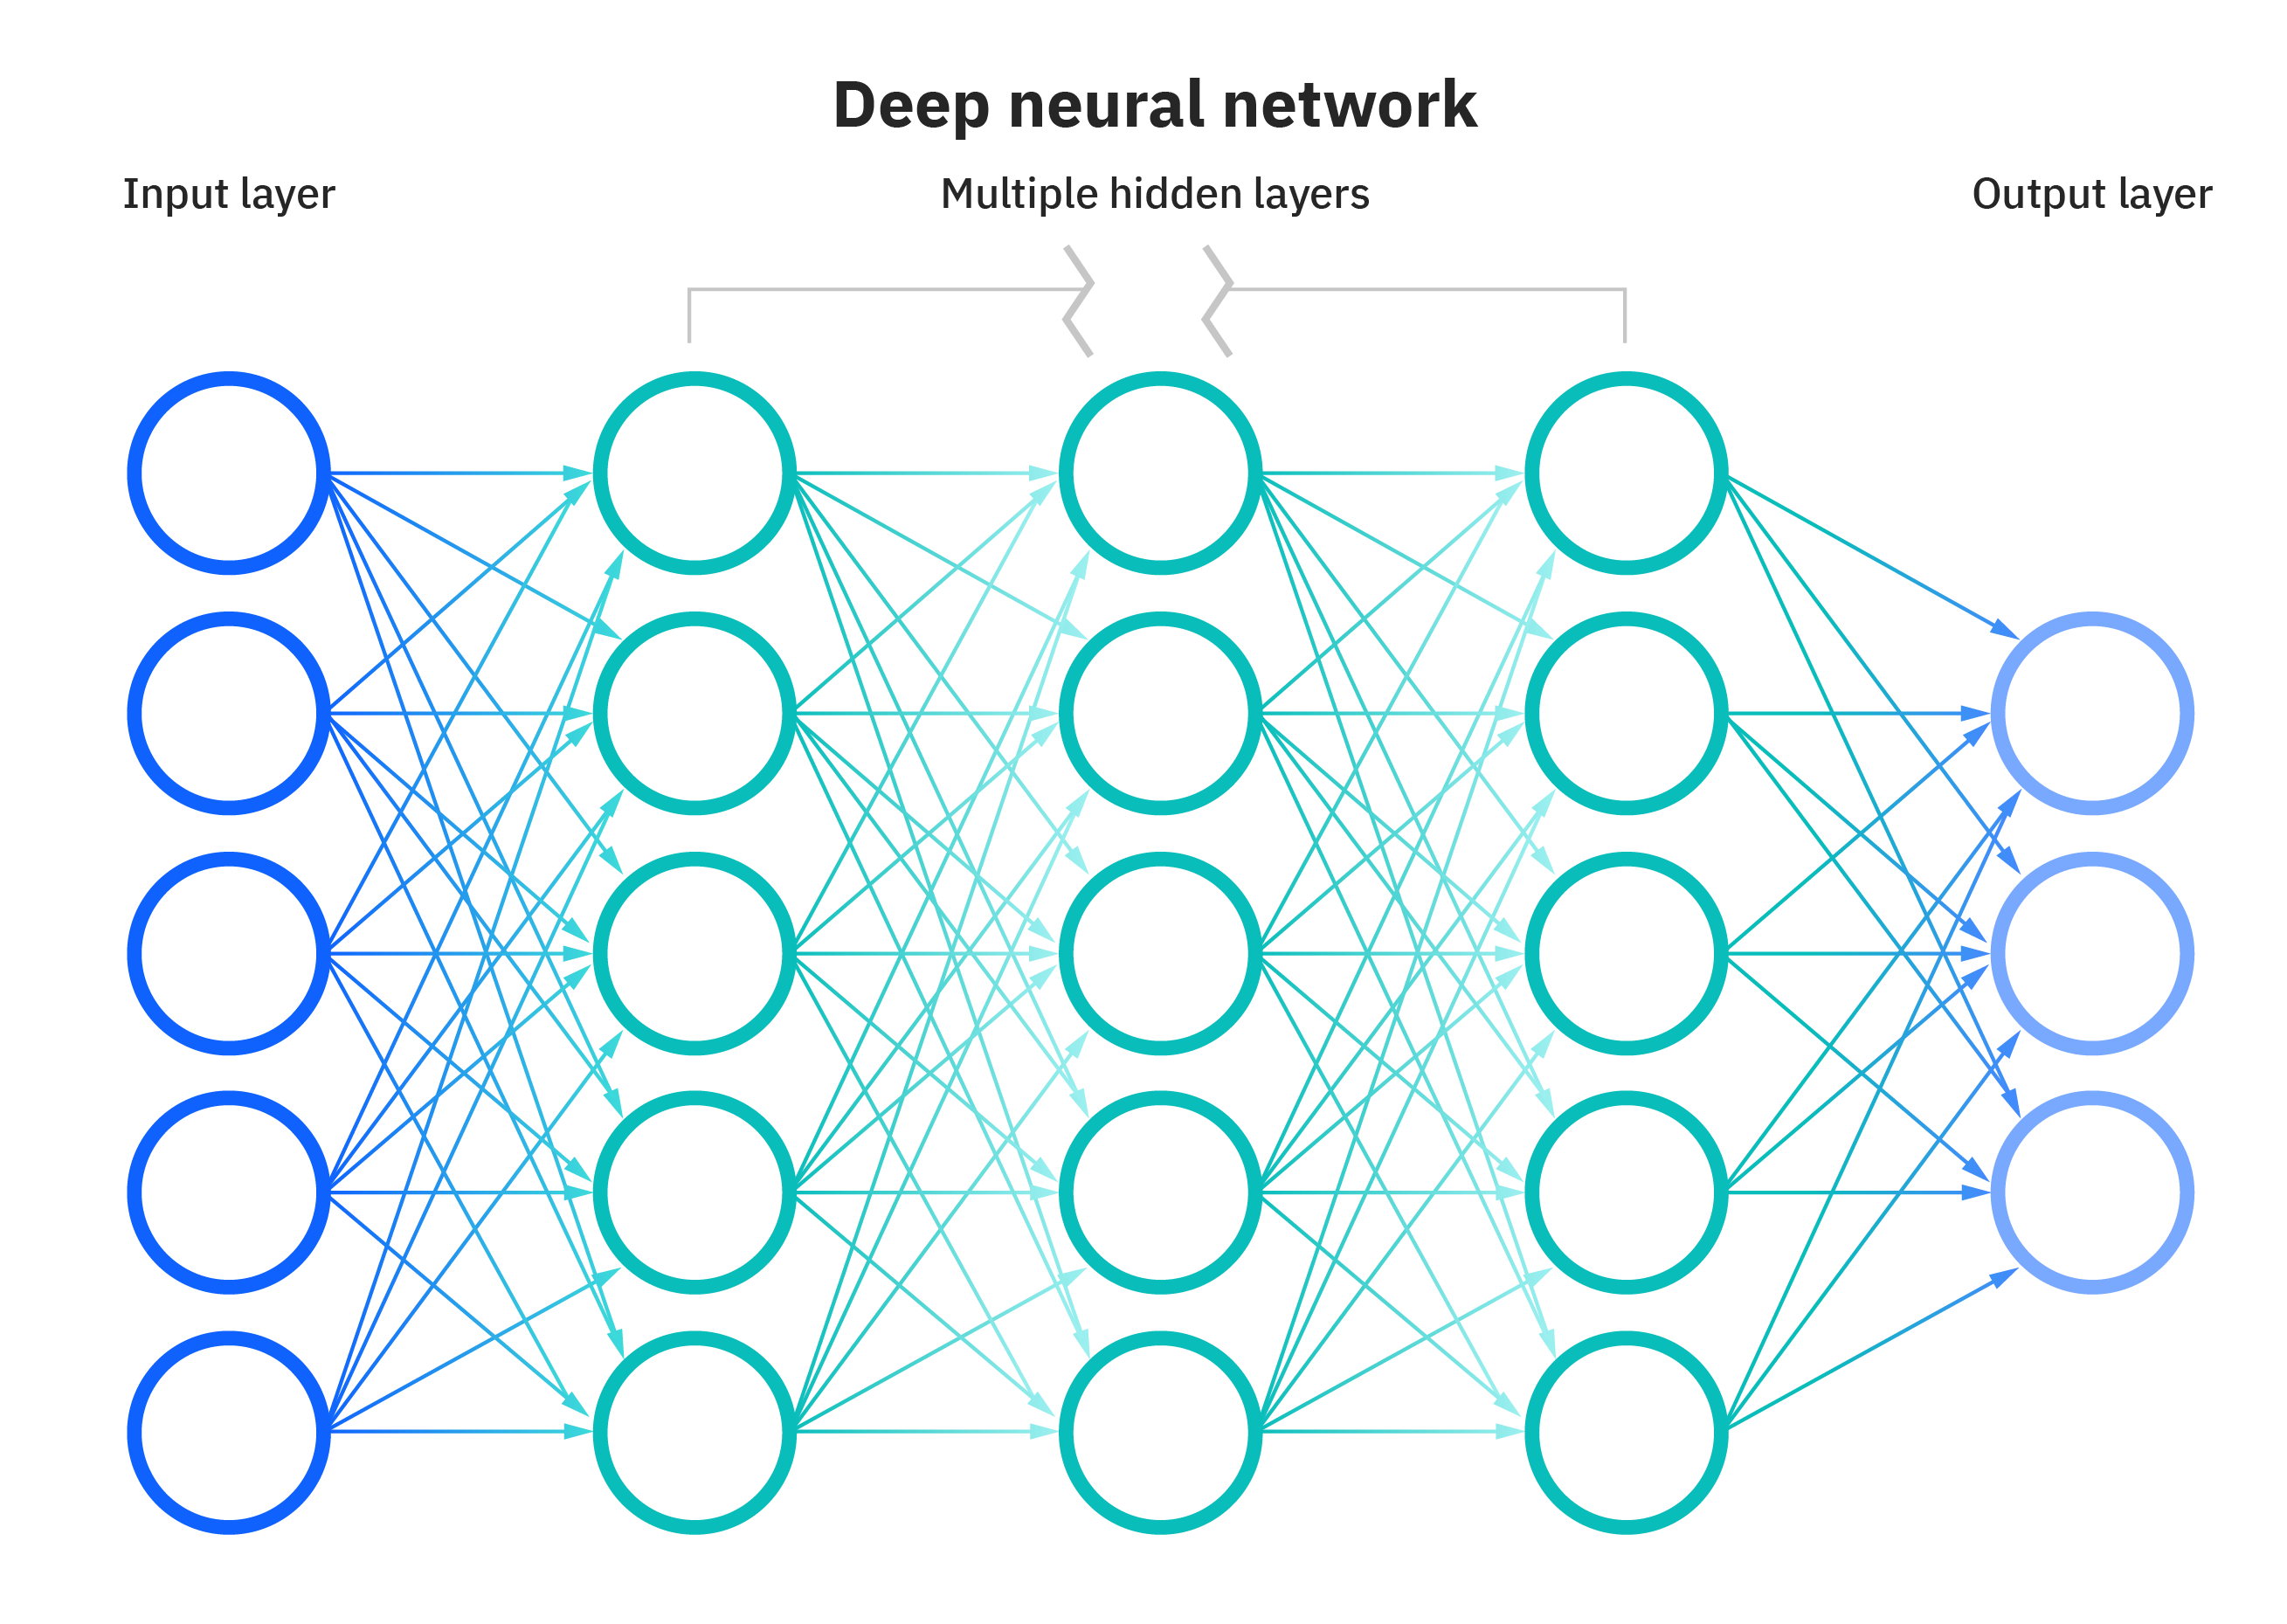
\includegraphics[width=0.75\textwidth]{Figures/NeuralNetwork.png}
	\caption{An illustration of a neural network}
\end{figure}
\FloatBarrier

\acrshort{nn} are comprised of a node layers, containing an input layer, one or more hidden layers, and an output layer. Each node, or artificial neuron, connects to another and has an associated weight and threshold. These series of connections make the possibility to learn complex features from the dataset.

\subsubsection{Definition}
\acrfull{dl} is a subset of \acrfull{ml}, which is essentially a neural network with three or more layers. These neural networks attempt to simulate the behavior of the human brain—albeit far from matching its ability—allowing it to ``learn" from large amounts of data. 

\begin{figure}[H]
	\centering
	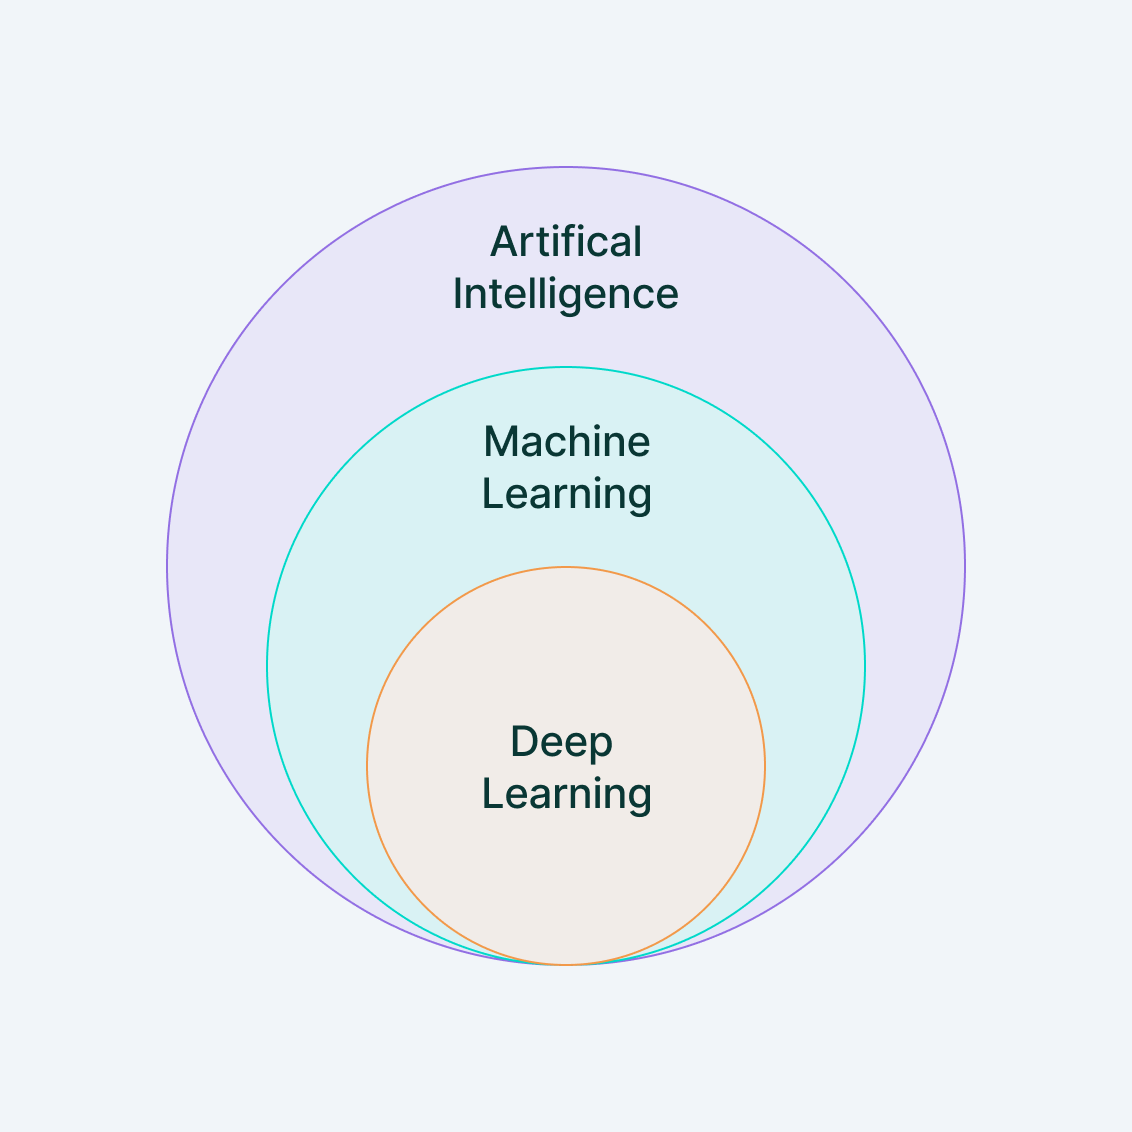
\includegraphics[width=0.5\textwidth]{Figures/AIHierarchy.png}
	\caption{Relation between \acrshort{ai}, \acrshort{ml} and \acrshort{dl}}
\end{figure}
\FloatBarrier

The term deep learning originated from new methods and strategies designed to generate these deep hierarchies of non-linear features by overcoming the problems with vanishing gradients so that we can train architectures with dozens of layers.

\begin{figure}[H]
	\centering
	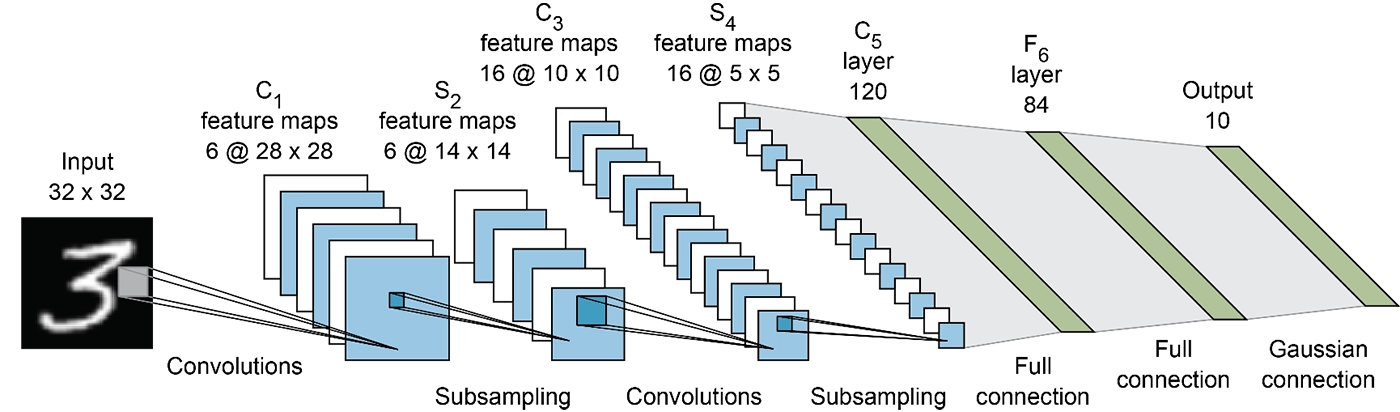
\includegraphics[width=0.75\textwidth]{Figures/CNN.png}
	\caption{An example of deep learning model}
\end{figure}
\FloatBarrier

\subsection{Reinforcement learning}
\acrfull{rl} is the science of decision making. It is about learning the optimal behavior in an environment to obtain maximum reward. This optimal behavior is learned through interactions with the environment and observations of how it responds, similar to children exploring the world around them and learning the actions that help them achieve a goal.

In the absence of a supervisor, the learner must independently discover the sequence of actions that maximize the reward. This discovery process is akin to a trial-and-error search. The quality of actions is measured by not just the immediate reward they return, but also the delayed reward they might fetch. As it can learn the actions that result in eventual success in an unseen environment without the help of a supervisor, reinforcement learning is a very powerful tool.
\begin{figure}[H]
	\centering
	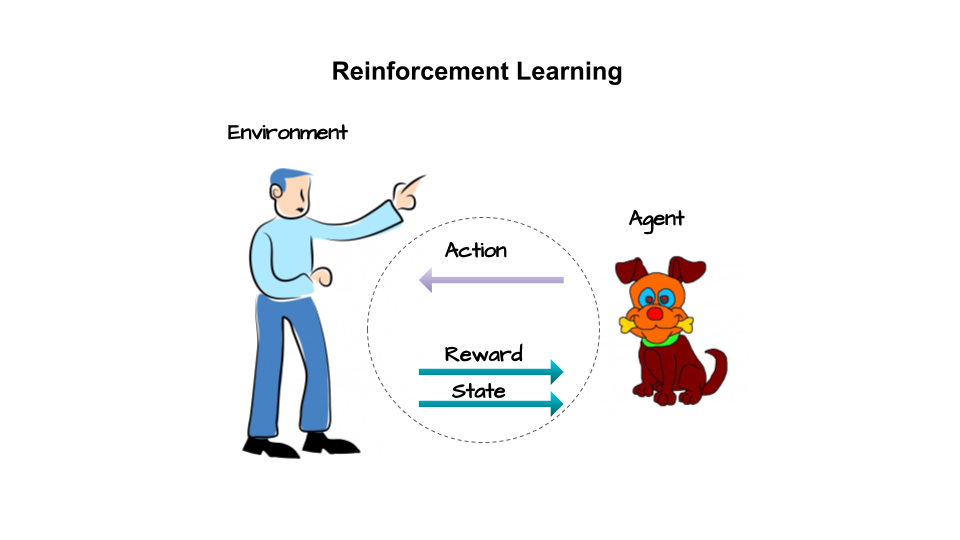
\includegraphics[width=0.75\textwidth]{Figures/RLCartoon.png}
	\caption{An example of a reinforcement learning system}
\end{figure}
\FloatBarrier


Due to its generality, reinforcement learning is studied in many disciplines, such as game theory, control theory, operations research, information theory, simulation-based optimization, multi-agent systems, swarm intelligence, and statistics. 
\subsection{Self Play}
In \acrfull{rl}, the term self-play describes a kind of \acrfull{mal} that
deploys an algorithm against copies of itself to test compatibility in various stochastic environments.

\acrfull{sp} rose to prominence after the great success of Alpha Go \cite{AlphaGo} and its subsequent version Alpha Zero \cite{AlphaZero}.

\begin{figure}[H]
	\centering
	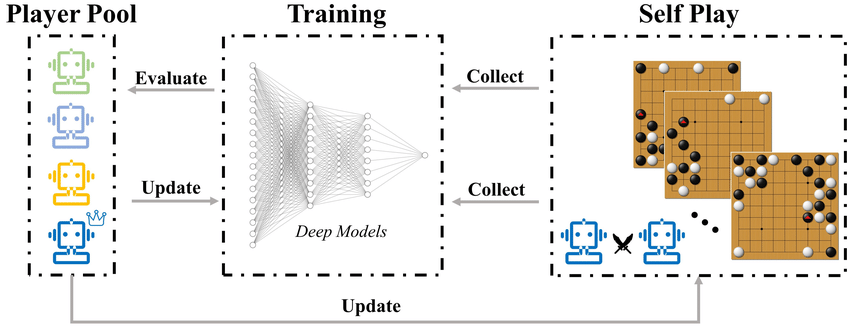
\includegraphics[width=0.75\textwidth]{Figures/AlphaZeroSelfPlay.png}
	\caption{Alpha Go pipeline}
	\scriptsize src: 
\end{figure}
\FloatBarrier

\section{Work methodologies}
This section is dedicated to describing the three methodologies we selected to conduct this
project, complemented by the Gantt chart which illustrates the distribution of our tasks
over the duration of the internship.

Each of the three methodologies we selected dealt with a different part of the project. These parts were very different in nature. As a result, we effectively considered them as distinct subprojects.

The choice of more than one methodology was necessary in our case, as each subproject had to be approached with a unique mindset.

\subsection{Agile Methodology}
As the first goal of the project was to implement and test a \acrshort{mpg} library, we followed the \textbf{Agile} methodology.

\begin{figure}[h]
	\centering
	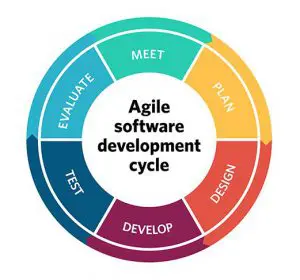
\includegraphics[width=0.4\textwidth]{Figures/Agile.png}
	\caption{Agile development cycle}
\end{figure}
\FloatBarrier

Agile methodology is a project management approach that prioritizes cross-functional collaboration and continuous improvement. It divides projects into smaller phases and guides teams through cycles of planning, execution, and evaluation.

Agile’s entire framework revolves around the program’s core values. Many of the Agile Principles are directly based on these values:
\subsection{Crisp-DM}
The second subproject was to analyse, and implement a reinforcement learning model for \acrshortpl{mpg}. For that part, we used the \textbf{Crisp-DM}

CRISP-DM, which stands for Cross-Industry Standard Process for Data Mining, is an industry-proven way to guide the data mining efforts.

\begin{figure}[h]
	\centering
	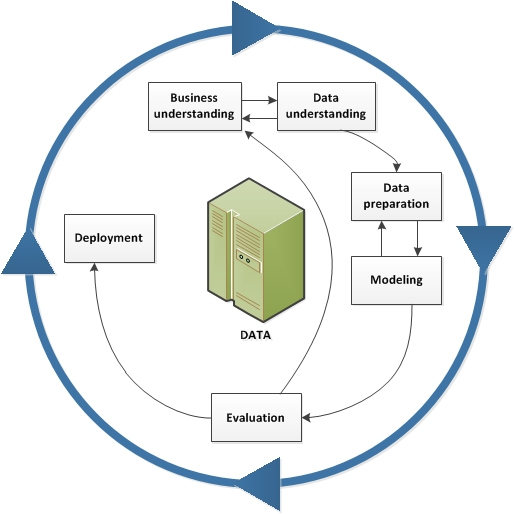
\includegraphics[width=0.5\textwidth]{Figures/CRISP_DM.jpg}
	\caption{Agile development cycle}
\end{figure}
\FloatBarrier

As a methodology, it includes descriptions of the typical phases of a project, the tasks involved with each phase, and an explanation of the relationships between these tasks.
As a process model, CRISP-DM provides an overview of the data mining life cycle.
%Add ,right=0.35
\newgeometry{left=0.35cm,bottom=0.5cm}
\thispagestyle{empty}

\begin{landscape}
	
\begin{figure}
	\noindent
					\vspace*{-2cm}
	\hspace{4.35cm}
		\makebox[\textheight]{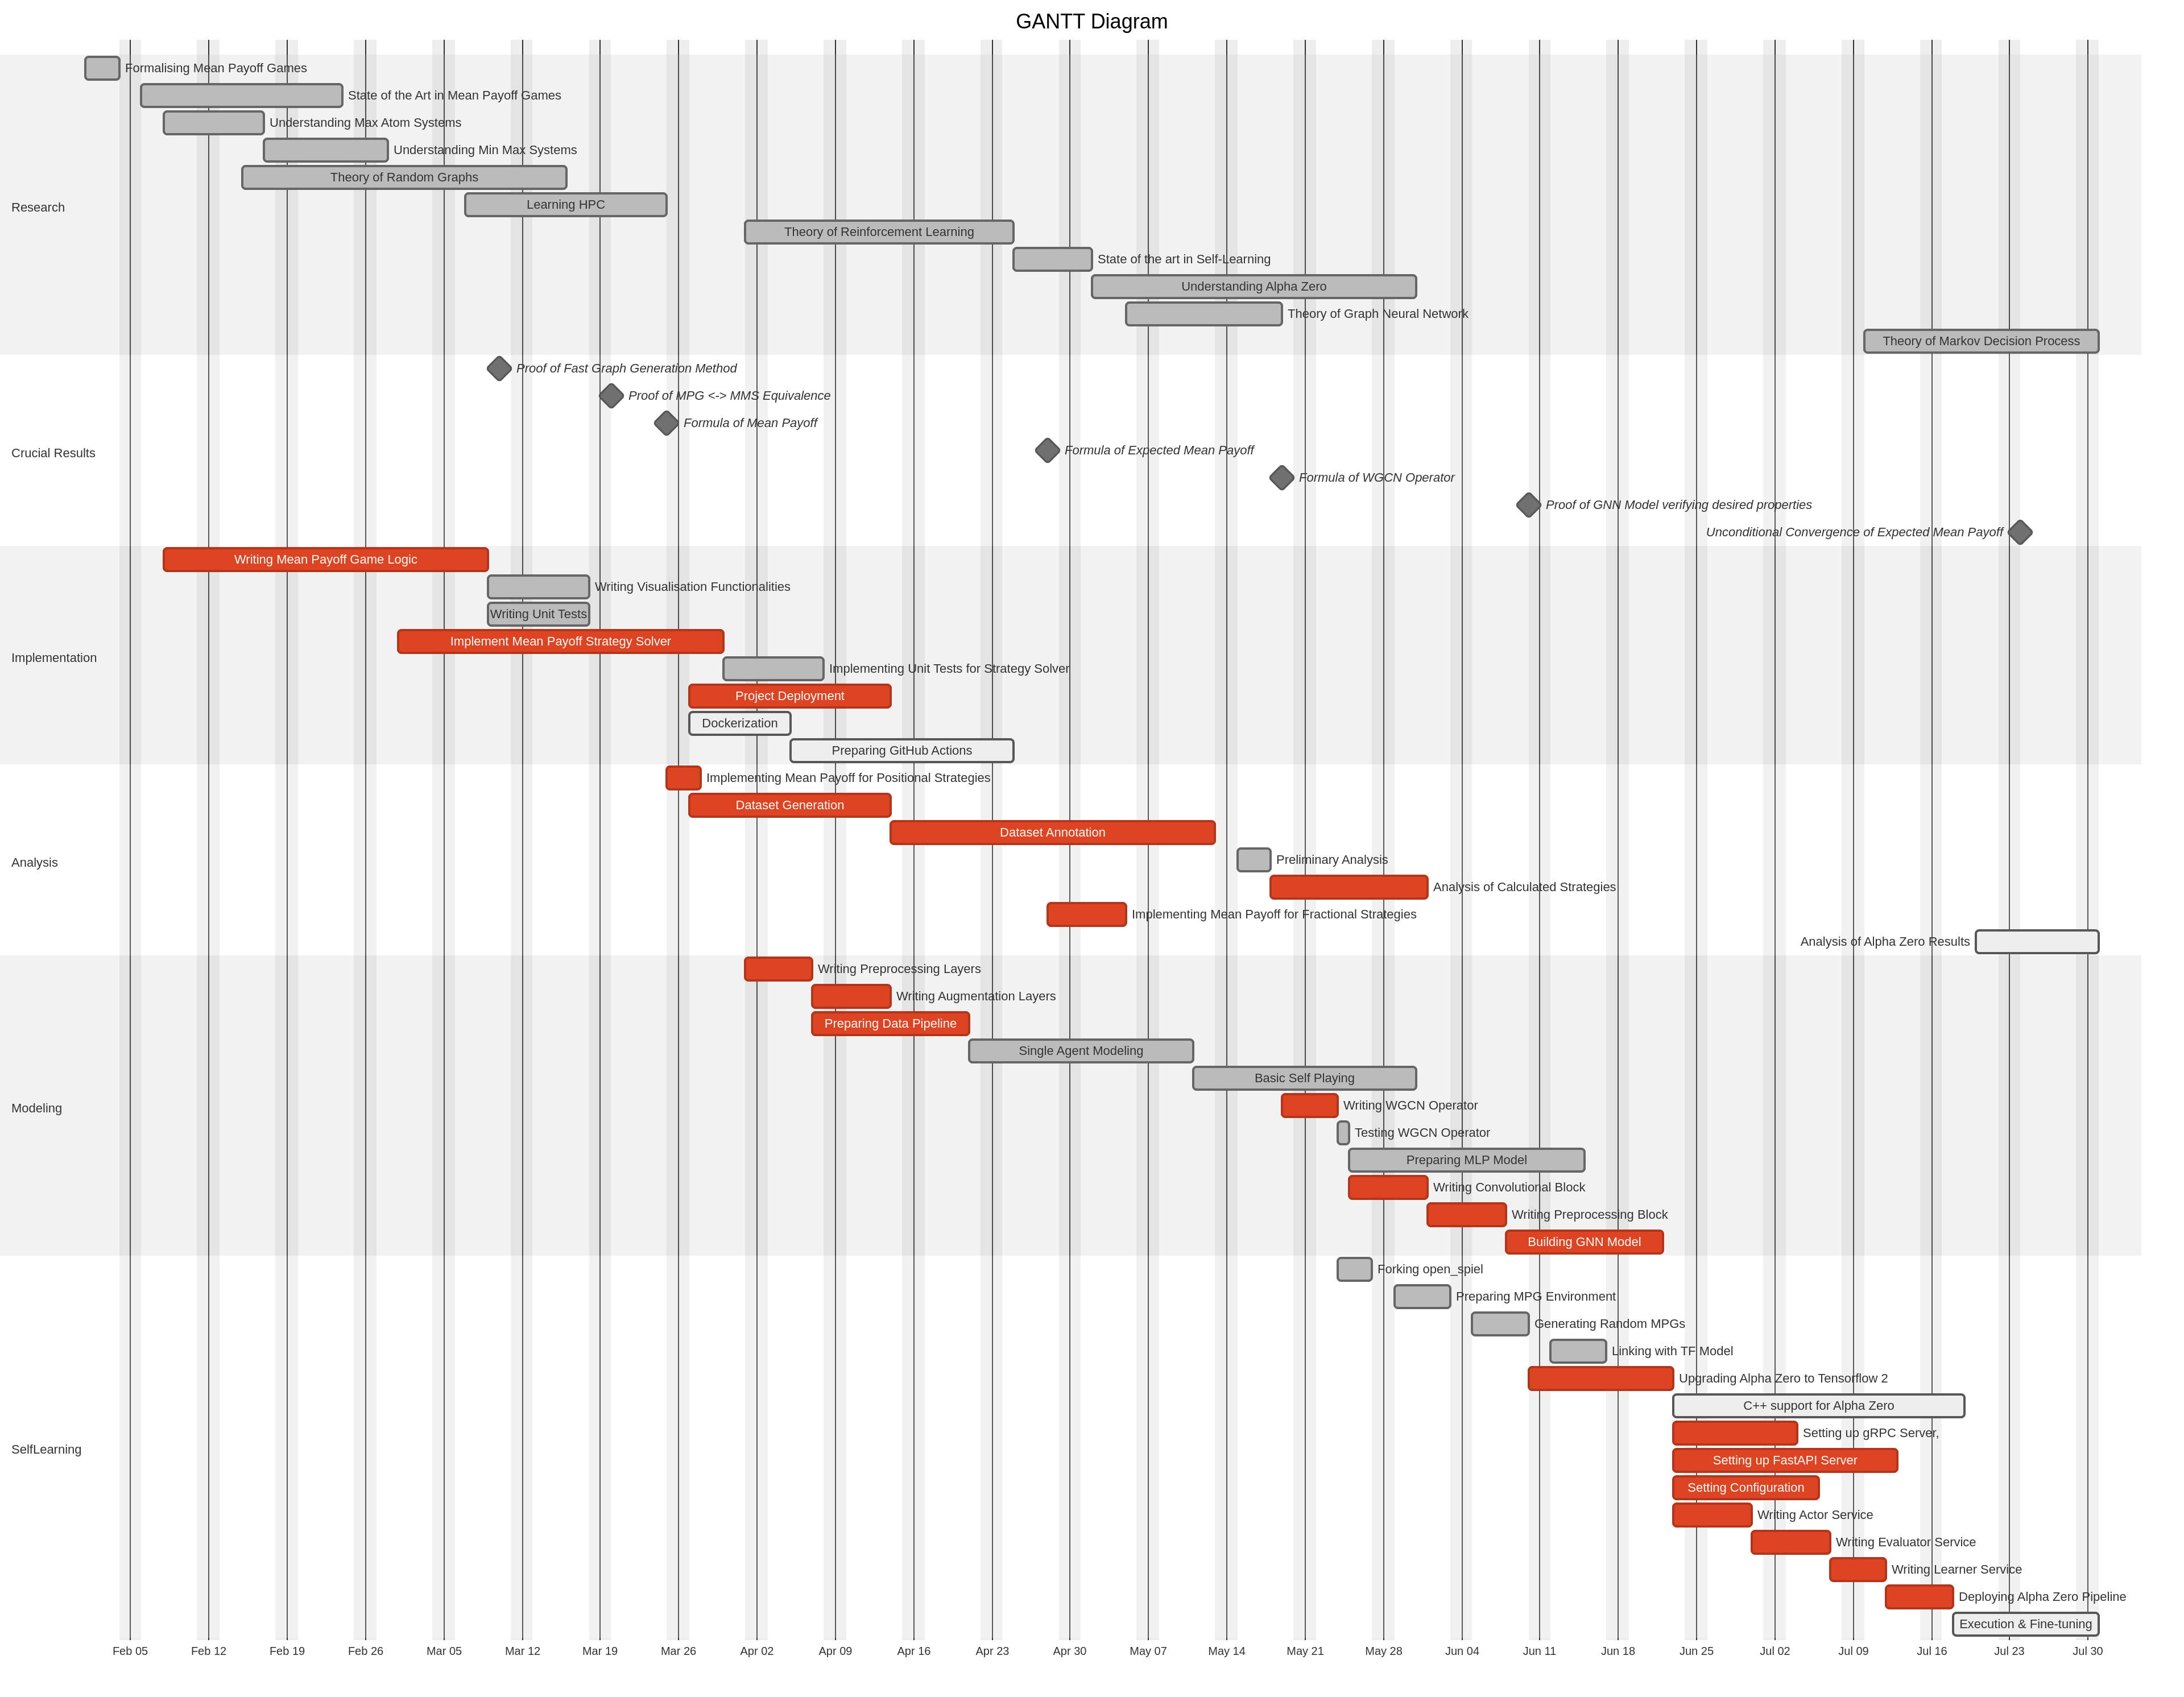
\includegraphics[height=1.2 \textheight]{Figures/Gant.png}}

	\caption{Gantt diagram}

\end{figure}

\end{landscape}
\restoregeometry
\chapter{Analysis \& Implementation}
\section{Introduction}

\section{Formalisation}
To define a Mean Payoff Game, we will start by formalising a weighted di-graph\footnote{Directed Graph}.

\subsection{Di-Graph}
A Weighted Di-Graph $G$ is a tuple $(\VertexSet,\EdgeSet,W)$ where:

\begin{itemize}
		\item $\VertexSet$ is the set of vertices.
		\item $\EdgeSet \subseteq \VertexSet\times \VertexSet$ is the set of edges.
		\item $W:\EdgeSet\rightarrow \mathbb{G}$ is the weight function, assigning a weight for every edge, with $\mathbb{G}$ some ordered abelian group\footnote{This definition is too general. We will only consider $\mathbb{G}\in \{\mathbb{Z},\mathbb{Q},\mathbb{R}\}.$ Also, $\mathbb{G}$ itself should be clear from the context.}. 
\end{itemize}
\subsection{Mean Payoff Game}
Formally, a \textbf{Mean Payoff Graph} is a tuple $(\VertexSet,\EdgeSet,W,\PlayerSet,s,p)$ where:
\begin{itemize}
	\item $\mathcal{G}=(\VertexSet,\EdgeSet,W)$ is a di-graph.
		\item $s\in \VertexSet$ denotes the starting position.
	\item $\PlayerSet=\{\text{Max},\text{Min}\}$ is the set of players.
	\item $p\in \PlayerSet$ the starting player
\end{itemize}


A  \textbf{Mean Payoff Game} is a perfect information, zero-sum, turn based game played indefinitively on a Mean Payoff Graph as follow:
\begin{itemize}
\item The game starts at $u_0=s$, with player $p_0=p$ starting.
\item For each $n\in\mathbb{N},$ Player $p_n$ will choose a vertex $u_{n+1}\in \Adj u_n,$ with a payoff $w_n=W(u_n,u_{n+1})$
\item The winner of the game will be determined by the Mean Payoff. There are different winning conditions.
\end{itemize}

\begin{table}[h]
	\small
	\begin{tabularx}{\textwidth}{| p{2cm} | X | X | X |}
		\hline
		
		Name & $\Max$ winning criteria & $\Min$ winning criteria & Draw criteria  \\
		\hline
		$C_1$ & \begin{equation*}
			\liminf_{n\in\mathbb{N}^*} \frac{1}{n}\sum_{k=0}^{n-1} w_k \ge 0
		\end{equation*} & \begin{equation*}
		\liminf_{n\in\mathbb{N}^*} \frac{1}{n}\sum_{k=0}^{n-1} w_k < 0
		\end{equation*} & \cellcolor{gray!75} \\
		\hline
		$C_2$ & \begin{equation*}
			\liminf_{n\in\mathbb{N}^*} \frac{1}{n}\sum_{k=0}^{n-1} w_k > 0
		\end{equation*} & \begin{equation*}
			\liminf_{n\in\mathbb{N}^*} \frac{1}{n}\sum_{k=0}^{n-1} w_k < 0
		\end{equation*} & \begin{equation*}
		\liminf_{n\in\mathbb{N}^*} \frac{1}{n}\sum_{k=0}^{n-1} w_k = 0
		\end{equation*} \\
		\hline
		 $C_3$ & \begin{equation*}
		 	\liminf_{n\in\mathbb{N}^*} \frac{1}{n}\sum_{k=0}^{n-1} w_k > 0
		 \end{equation*} & \begin{equation*}
		 	\limsup_{n\in\mathbb{N}^*} \frac{1}{n}\sum_{k=0}^{n-1} w_k < 0
		 \end{equation*} & \begin{equation*}
		 \begin{cases} 
		 	\displaystyle \liminf_{n\in\mathbb{N}^*} \frac{1}{n}\sum_{k=0}^{n-1} w_k \le 0 \\
		 	 \displaystyle \limsup_{n\in\mathbb{N}^*} \frac{1}{n}\sum_{k=0}^{n-1} w_k \ge 0
		 \end{cases}
		 \end{equation*}\\
		\hline
	\end{tabularx}
	\caption{Winning conditions for Mean Payoff Games
		\label{table:WinningConditions}}
\end{table}
Here, table \ref{table:WinningConditions} gives the different winning criteria that we have considered:
\begin{itemize}
	\item $C_1$ was used in \cite{MPGMaxAtom} to calculate the optimal strategy for player $\Max$
	\item $C_2$ is modification of $C_1$ that introduces the possibility of drawing.
	\item $C_3$ is symmetric\footnote{It does not give an advantage towards any player.}, and will be used for our machine learning. It was referenced in \cite{TropicalCSP}.
\end{itemize}
Now, there is a slight difference between the three winning conditions.
\newline For example, an optimal strategy with respect to $C_1$ may not be optimal with respect to $C_2$. While this can happen, it is unlikely.
\newline What about $C_2$ and $C_3$? As different as they appear, they are equivalent in the scope of this report\footnote{They are still different conditions in general.}.
This is demonstrated in \ref{section:Formalisation:MeanPayoff}.
\subsection{Well Foundness}
It is not very clear from the definition that the game is well founded. \newline
In fact, there are choices for which the mean payoff does not converge. That is the sequence $\left(\frac{1}{n}\sum_{k=0}^{n-1} w_k \right)_{n\in\mathbb{N}^*}$ does not converge. \newline One such example is the sequence defined by:
$$
w_n=(-1)^{\lfloor  \log_2 (n+1)\rfloor}
$$
For that sequence, the $(2^r-1)$-step mean payoff is equal to:
\begin{align*}
	\sum_{k=0}^{2^r-2} w_k &= 	\sum_{k=1}^{2^r-1}(-1)^{\lfloor  \log_2 (k)\rfloor} = \sum_{i=0}^{r-1}\sum_{j=2^{i}}^{2^{i+1}-1}(-1)^{\lfloor  \log_2 (j)\rfloor} \\
	&=\sum_{i=0}^{r-1}\sum_{j=2^{i}}^{2^{i+1}-1}(-1)^i =\sum_{i=0}^{r-1}(2^{i+1}-2^i)(-1^i) \\
	&=\sum_{i=0}^{r-1}(-2)^i = \frac{1-(-2)^r}{3} \\
	\implies \frac{1}{2^r-1}\sum_{k=0}^{2^r-2} w_k  &= \frac{1}{3} \cdot \frac{1-(-2)^r}{2^r-1} = \frac{1}{3} \cdot \frac{2^{-r}-(-1)^r}{1-2^{-r}}
\end{align*}
That sequence has two accumulation points $\pm \frac{1}{3},$ and thus, it does not converge.

On the other hand, the introduction of the supremum and infimum operators in the table \ref{table:WinningConditions} will solve the convergence problem, as the resulting sequences will become monotone.

An example of an execution that gives a rise to such payoffs is the following Meab Payoff Game instance\footnote{Note that the proposed pair of strategies is odd in the sense that it appears that both players cooperated on the construction of non-convergent mean payoffs instead of trying ot win the game.}:
\begin{figure}[H]
	\centering
	\begin{subfigure}[b]{0.45\textwidth}
		\raggedleft
		\begin{tikzpicture}[->,>=stealth',shorten >=1pt,auto,node distance=4cm,
			thick,main node/.style={circle,draw,font=\Large\bfseries}]
			\node[main node, fill=gray!50] (1) {$0$}; 
			\node[main node] (2) [right of =1] {$1$}; 
			\path (1) edge [loop above] node {1} (1)
			edge [bend right] node [below] {-1} (2)
			(2) edge [bend right] node [above] {1} (1)
			edge [loop above] node {-1} (2);
		\end{tikzpicture} 
		\caption{Representation of the Mean Payoff Game}
	\end{subfigure}
  \hfill
	\begin{subfigure}[b]{0.45\textwidth}
		\raggedright
		\small
		Pair of strategies defined as:
		\begin{align*}
		\Phi: &V^+ \times P \rightarrow V \\
		 &(s_0\dots s_r, p) \rightarrow B(r)\bmod 2
		\end{align*}
		\scriptsize
		With $B(r)$ the position of the left-most bit in the binary representation of $r$
		\caption{Definition of both strategies}
	\end{subfigure}
	\caption{An example of an execution with non-convergent Mean Payoffs
			\label{fig:MeanPayoffNonConvergence}}
\end{figure}
\subsection{Properties}
A Mean Payoff Game has many properties that are interesting from a game theory perspective.
\subsubsection{Two Player}
The game is a two player game.
\subsubsection{Turn Based}

\subsection{Symmetries}
Mean Payoff Games exhibits many natural symmetries.
\subsubsection{Duality}
The main symmetry is the duality between 
$\Max$ and $\Min.$
\newline For this we will define the dual $\bar{G}$ of a mean payoff game $G=(\VertexSet,\EdgeSet,W\PlayerSet,s,p)$ as the following:
$$
\bar{G}= (\VertexSet,\EdgeSet,-W,s,\bar{p})
$$
This duality is important due to the following theorem.
\begin{theorem}
	For every mean payoff game $G$, the objective of player $\Max$ is equivalent to the objective of player $\Min$ in $\bar{G}.$
\end{theorem}
With that, there is not any major difference between $\Max$ and $\Min$ from a theoretical point of view.
\newline In fact, without any loss of generality, we can assume that $\Max$ is the starting player. And this is what we will do by default in this report.
\begin{figure}
	\begin{tikzpicture}[->,>=stealth',shorten >=1pt,auto,node distance=2cm,
		thick,main node/.style={circle,draw,font=\Large\bfseries}]
		\node[main node, fill=gray!50] (1) {$0$}; 
		\node[main node] (2) [above of =1] {$1$}; 
		\node[main node] (3) [above right of =2] {$2$}; 
		\node[main node] (4) [above of =3] {$3$}; 
		\node[main node] (5) [above left of =2] {$4$}; 
		\node[main node] (6) [above of =5] {$5$}; 
		\node[main node] (7) [above of =6]{$6$}; 
		\path (1) edge node {2} (2)
		(2) edge node {3} (3)
			edge node {3} (5)
		(3) edge [bend left] node {-5} (4)
			edge [bend left] node {-5} (2)
		(4) edge [bend left] node {-5} (2)
			edge [bend left] node {-2} (4)
		(5) edge node {3} (6)
			edge [bend left=25] node {3} (7)
		(6) edge node {3} (1)
		(7) edge [bend right=45] node {3} (1);
	\end{tikzpicture} 
\end{figure}

\subsection{Strategy}
\subsubsection{Deterministic Strategies}
Let $p$ be a player. \newline 
A (deterministic) strategy is a function $\Pi^{p}:\VertexSet^+\rightarrow \VertexSet$ such that:
$$
\forall v_0\dots v_r\in \VertexSet^+, \quad \Pi_p(v_0\dots v_r) \in \Adj v
$$	
If the strategy does only depend on the current vertex, we say it is a memoryless (deterministic) strategy.  $\Pi:\VertexSet\rightarrow \VertexSet$
\newline In this report, we will use the term positional strategies as an alias for memoryless deterministic strategies, which is conforming to the established litterature of mean payoff games.
\newline Positional strategies are crucial for our analysis as a result of the following theorem.
\begin{theorem}
	\label{theorem:OptimalStrategy}
	For all Mean Payoff Games, each player has an optimal positional strategy.
\end{theorem}

\subsubsection{Probabilistic Strategies}
A probabilistic strategy is a random process that assigns for each sequence of vertices $v\in\mathcal{V}$ a probability distribution over $\Adj v.$ This constitutes the most general strategy of a player:
$$
\forall v_0\dots v_r\in \VertexSet^+, \quad \Pi_p(v_0\dots v_r) \in \Distribution{\Adj v}
$$
\subsubsection{Considered Strategies}
Strategies that depends in complete past histories are in general intractable. For Mean Payoff Game, it is proven that the optimal strategy is a \textbf{deterministic} and \textbf{memoryless}.
\newline For that we will only consider \textbf{memoryless} strategies. And for the scope of this report:
\begin{itemize}
	\item A deterministic strategy should refer to memoryless deterministic strategy.
	\item A probabilistic strategy should refer to memoryless probabilistic strategy.
	\item A strategy should refer to memoryless deterministic strategy.
\end{itemize}
We will still consider (memoryless) probabilistic strategies as they reside in a smooth space, and thus they can be used for machine learning purposes.
\subsubsection{Deterministic Optimal Strategy}
There are three kinds of optimality:
\paragraph{Weak Optimality}: In the deterministic case, a strategy $\Phi$ of player $p\in \PlayerSet$ is weakly optimal if one of the following is true:
\begin{itemize}
	\item For each strategy $\Phi^{p}$ of player $p,$ player $\bar{p}$ can win the game by finding a countering strategy $\Phi^{\bar{p}}.$
	\item Player $p$ will not lose the game no matter his opponent's strategy
\end{itemize}

\paragraph{Strong Optimality}: In the deterministic case, a strategy $\Phi$ of player $p\in \PlayerSet$ is strongly optimal if one of the following is true:
\begin{itemize}
	\item For each strategy $\Phi^{p}$ of player $p,$ player $\bar{p}$ can win or tie the game by finding a countering strategy $\Phi^{\bar{p}}.$
	\item Player $p$ will win the game no matter his opponent's strategy
\end{itemize}

\paragraph{Payoff Optimality}: In the deterministic case, a strategy $\Phi$ of player $p\in \PlayerSet$ is payoff optimal if independently of $\bar{p}$'s strategy it:
\begin{itemize}
	\item Maximises the Mean Payoff if $p=\text{Min}$ 
	\item Minimises the Mean Payoff otherwise
\end{itemize}
Now we have the following hiearchy considering the set of optimal strategies:
$$
\forall \text{Mean Payoff Game}\ G,\forall p\in \PlayerSet,\quad \PayoffOptimal(G,p) \subseteq \StrongOptimal(G,p) \subseteq \WeakOptimal(G,p)
$$
\subsection{Mean Payoff}
\label{section:Formalisation:MeanPayoff}
We have used the word ``Mean Payoff" extensively, and they are the central entity in mean payoff games\footnote{This explains the name ``mean payoff game".} but we still did not define it.
\newline We had to delay the definition as it requires the knowledge of the mechanics of the game, and how strategies work. This section will define and formalize the mean payoff, and highlights its relevance.
\subsubsection{Mean Payoff}
For a mean payoff game $G$, with a deterministic pair of strategies $(\Phi^{\Max},\Phi^{\Min}),$ we will define two terms $v^+(G,\Phi^{\Max},\Phi^{\Min})$ and $v^-(G,\Phi^{\Max},\Phi^{\Min})$ as follow\footnote{For probabilistic strategies, both terms are random variables, so we will be interested in their expected values.}:
\begin{align*}
v^+(G,\Phi^{\Max},\Phi^{\Min}) &=\limsup_{n\in\mathbb{N}^*} \frac{1}{n}\sum_{k=0}^{n-1} w_k \\
v^-(G,\Phi^{\Max},\Phi^{\Min}) &=\liminf_{n\in\mathbb{N}^*} \frac{1}{n}\sum_{k=0}^{n-1} w_k
\end{align*} 
Where $(w_n)_{n\in\mathbb{N}}$ is the sequence of payoffs generated by the instance.
\newline These two terms were used in table $\ref{table:WinningConditions}$ when discussing the winning conditions, and we will call them respectively the supremum mean payoff, and the infimum mean payoff. 
\begin{theorem}
	For every mean payoff game $G$, and every pair of strategies $(\Phi^{\Max},\Phi^{\Min})$, both the supremum mean payoff $v^+(G,\Phi^{\Max},\Phi^{\Min})$ and the infimum mean payoff $v^-(G,\Phi^{\Max},\Phi^{\Min})$ are guaranteed to exist, and:
	\begin{equation}
		\label{eqn:InfSupRelationMeanPayoff}
		v^-(G,\Phi^{\Max},\Phi^{\Min}) \le v^+(G,\Phi^{\Max},\Phi^{\Min})
	\end{equation}
\end{theorem}
If both terms are equal in equation  \eqref{eqn:InfSupRelationMeanPayoff}, we say that the game instance has a mean payoff $v(G,\Phi^{\Max},\Phi^{\Min})=v^-(G,\Phi^{\Max},\Phi^{\Min})=v^+(G,\Phi^{\Max},\Phi^{\Min}).$

\subsubsection{Convergence Issues}
This mean payoff itself is the heart of mean payoff games. A major problem lies in the fact that the existence of a mean payoff is not guaranteed, and an example for such case is found in the \newline figure \ref{fig:MeanPayoffNonConvergence}.
\newline Now, fortunately, this is not an issue, as we are interested in good strategies. Theorem \ref{theorem:OptimalStrategy} proven in \cite{PositionalStrategies} states that for each player, the set of optimal strategies contains a positional one. This is a very important result as we can limit the domain of our optimization problem\footnote{The problem of finding optimal strategies} to the more tractable positional\footnote{memoryless and deterministic} and behavioural\footnote{memoryless and probabilistic} strategies.
\newline We start by tackling the existence of the mean payoff for positional strategies in the the following theorem:
\begin{theorem}
	\label{theorem:MeanPayoffExistence}
	For every mean payoff $G$, and a pair of positional strategies $(\Phi^{\Max},\Phi^{\Min}),$ the mean payoff $v(G,\Phi^{\Max},\Phi^{\Min})$ exists.
\end{theorem}
We will give a constructive proof of theorem \ref{theorem:MeanPayoffExistence} in section \ref{section:StrategyEvalution}. We will also provide a linear algorithm for its calculation.
\newline Furthermore, in our machine learning model, we will approach the problem using behavioural strategies. Also luckily, its existence is guaranteed by the following theorem:
\begin{theorem}
	\label{theorem:MeanPayoffExistenceProbabilstic}
	For every mean payoff $G$, and a pair of behavioural strategies $(\Pi^{\Max},\Pi^{\Min}),$ the expected mean payoff $\mathbb{E}[v(G,\Pi^{\Max},\Pi^{\Min})]$ exists.
\end{theorem}
Unlike theorem \ref{theorem:MeanPayoffExistence} theorem \ref{theorem:MeanPayoffExistenceProbabilstic} was very challenging to prove, and we were not able to find a direct proof in the literature. We had some probabilistic arguments that affirmed the result for almost all mean payoff games. This alone was enough for us to use it as a metric for probabilistic strategies.
\newline Eventually, we were able to give a formal proof, which is detailed in the appendix \ref{appendix:Probabilistic:Strategies}.
\subsubsection{Game Value}
By combining both theorems \ref{theorem:OptimalStrategy} and \ref{theorem:MeanPayoffExistence}, there is a mean payoff $v(G)$ that both players are guaranteed to achieve if they play optimally:
\begin{align*}
\exists \Phi^{\Max},\forall \Phi^ {\Min}, & \quad v^-(G,\Phi^{\Max},\Phi^{\Min}) \ge v(G) \\
\exists \Phi^{\Min},\forall \Phi^{\Max}, & \quad v^+(G,\Phi^{\Max},\Phi^{\Min}) \le v(G) 
\end{align*}
Such mean payoff is called the value of the game. This value determines the winner of the game assuming both players play optimally.
\section{Evaluating Strategies}
\label{section:StrategyEvalution}
Suppose we have a pair of potentially probabilitic strategies $(\Phi^{\Max},\Phi^{\Min}).$ The problem is to evaluate the winner without doing an infinite simulation of the game. 
\subsection{Monte-Carlo Simulations}
This is the most intuitive evaluation method 
\subsection{Positional Strategies}
If both strategies are deterministic and memoryless. Then the generated sequence of vertices $(s_n)_{n\in\mathbb{N}}$ will be completely determined by the recurrence relation:
$$
s_n=\begin{cases}
	s & \text{if } \space n=0 \\
	\Phi^{\Max}(s_{n-1})& \text{if}\ n \ \text{is odd} \\
	\Phi^{\Min} (s_{n-1}) & \text{otherwise}
\end{cases}
$$
This can be represented in the compact form:
$$
\forall n\in\mathbb{N}^*,\quad \left(s_n, p_n
\right) = \left(\Phi^{p_{n-1}}(s_{n-1}), \bar{p}_{n-1}\right) = F(s_{n-1},p_{n-1})
$$

Since $\mathcal{V} \times \mathcal{P}$ is a finite set and $F$ is a function, such sequence will be eventually periodic, that is:
$$
\exists N \in \mathbb{N},\exists T\in\mathbb{N}^*/\quad \forall n\in\mathbb{N}_{\ge N},\quad (s_{n},p_{n})=(s_{n+T},p_{n+T})
$$

We can calculate its eventual period using the turtle hare algorithm. %Reference?

Now, the mean payoff will be equal to the mean of weights that appears on the cycle. \newline
This can be proven as follow.:
% w_n has offset N
\begin{align*}
	S_{aT+b+N}&=\sum_{k=0}^{aT+b+N-1} w_{k} \\
	&= \sum_{k=0}^{N-1}  w_{k}  + \sum_{k=0}^{aT+b-1} w_{k+N} \\
	&= \sum_{k=0}^{N-1}  w_{k}  + a\sum_{r=0}^{T-1} w_{r+N} +  \sum_{r=0}^{b-1} w_{r+N} \\
	\implies \left \lvert S_{n+N}- \lfloor \frac{n}{T}\rfloor \sum_{r=0}^T w_{k+N}  \right\rvert &\le (N+T-1) \max_{(u,v)\mathcal{E}} \lvert \mathcal{W}(u,v) \rvert  \\
	&\le (N+T-1) \lVert \mathcal{W} \rVert_{\infty} \\
\implies \left \lvert \frac{1}{n+N}S_{n+N}-\frac{1}{n+N} \cdot \lfloor \frac{n}{T}\rfloor \sum_{r=0}^{T-1} w_{k+N}  \right\rvert &\le \frac{N+T-1}{n+N}  \lVert \mathcal{W} \rVert_{\infty} \\
\end{align*}
Now it can be proven that:
$$
\lim_{n\rightarrow +\infty } \frac{1}{n+N} \cdot \lfloor \frac{n}{T}\rfloor \sum_{r=0}^T w_{k+N}  = \frac{1}{T}\sum_{r=0}^{T-1}w_{r+N}
$$
With that:
$$
\lim_{n\rightarrow +\infty} \frac{1}{n}\sum_{k=0}^{n-1} w_k=\frac{1}{T}\sum_{r=0}^{T-1}w_{r+N}  \quad \blacksquare
$$
Now, our algorithm will be composed of $3$ main parts:
\begin{itemize}
	\item Calculating the transition function $F:\VertexSet\times \PlayerSet \rightarrow \VertexSet\times \PlayerSet$. This is straightforward from the construction.
	\item Calculating the period and the offset of the sequence. We will use Floyd's cycle finding algorithm for that.
	\item Calculating the Mean Payoff
\end{itemize}
This is an illustrative implementation of our algorithm.
\begin{algorithm}
	\caption{Deterministic strategies evaluation}\label{alg:DeterministicEvaluation}
	\begin{algorithmic}
		\Require $G=(V,E,P,s,p)$ a mean payoff game
		\Require $(\Phi^{\text{Max}},\Phi^{\text{Min}})$ the edge probability 
		\Ensure $R$ The mean payoff  
		\State $F\leftarrow \text{Transition}(G,\Phi^{\text{Max}},\Phi^{\text{Min}})$\Comment{Calculate the transition function}

		\State $x_0\leftarrow (s,p)$
		\State $(T,r)\leftarrow \text{FloydCycleFinding}(F,x_0)$ \Comment{Find the period and the offset}
		\State $S\leftarrow 0$ \Comment{$S$ represents the cumulative payoffs along a cycle}
		\State $x\leftarrow x_0$
		\For {$k\in\{1,\dots,r\}$} \Comment{Advance until arriving to the cycle}
			\State $x\leftarrow F(x)$
		\EndFor
		\For {$k\in \{1,\dots,T\}$}
			\State $y\leftarrow \leftarrow F(x)$
			\State $u\leftarrow \displaystyle\projection_{V\times P\rightarrow V}(x)$ \Comment{Extracts the current vertex}
			\State $v\leftarrow \displaystyle\projection_{V\times P\rightarrow V}(y)$ \Comment{Extracts the next vertex}
			\State $S\leftarrow S+W(u,v)$
			\State $x\leftarrow y$
		\EndFor
		\State \Return $R\leftarrow \frac{S}{T}$
	\end{algorithmic}
\end{algorithm}
\FloatBarrier


\subsection{Probabilistic Strategies}
Due to the undeterministic nature of probabilistic strategies, it does not make sense to evaluate the mean payoffs, as different executions may lead to different mean payoffs. \newline
%Proof of discrete distribution nature
%My intuition says that it may not a distribution 
Instead, probabilistic strategies gives rise to a discrete distribution of mean payoffs. \newline
Now two closely related, but different evaluations are possible
\begin{itemize}
	\item Expected Mean Payoff
	\item Distribution of winners 
\end{itemize}
Now, with both strategies fixed. A Mean Payoff Game can be considered as a Markov Chain.

\begin{algorithm}
	\caption{Probabilistic strategies evaluation}\label{alg:ProbabilisticEvaluation}
	\begin{algorithmic}
		\Require $G=(V,E,P,s,p)$ a mean payoff game
		\Require $(\Pi^{\text{Max}},\Pi^{\text{Min}})$ the edge probability 
		\Ensure $\mathbb{E}[R]$ The expected mean payoff  
		\State $(A,W)\leftarrow \text{MRP}(G,\Phi^{\text{Max}},\Phi^{\text{Min}})$\Comment{Extract the MRP form. This is detailed in \ref{section:ProbabilisticStrategies:MRP}}
		
		\State $u\leftarrow (A\odot W)\ones$
		\State $X\leftarrow \text{NullSpace}(\Id - A)$ \Comment{Extract the kernel-basis of $\Id - A$}
		\State $Y\leftarrow \text{NullSpace}(\Id - A^T)$ \Comment{Extract the kernel-basis of $\Id - A^H.$}
		\State $T \leftarrow X(Y^TX)^{-1}Y^T$ \Comment{Calculate the limit $\displaystyle\lim_{n\rightarrow +\infty}\frac{1}{n}\sum_{k=0}^{n-1}A^k.$ This is detailed in \ref{section:ProbabilisticStrategies:AverageTimeReward}}
		\State \Return $\mathbb{E}[R]\leftarrow Tu$
	\end{algorithmic}
\end{algorithm}


\section{Countering Strategies}
By fixing the strategy of player $p\PlayerSet$ to $\Phi^p,$ then the Markov Game Process reduces to a Markov Decision Process, which can be solve by Linear Programming tools %Reference?
\newline Moreover, in a deterministic Mean Payoffs, a counter strategy can be calculated efficiently by reducing the problem to finding a negative cycle in a di-graph.
\subsection{Deterministic Counter Strategy}
For simplicity, we assume that $p=\Max,$ the same results apply for $\Min$ player.
\newline For a Mean Payoff Game $(\VertexSet,\EdgeSet,\PlayerSet,s,p'),$ we introduce the following graph:
$$
G'=\left(V,E',W'\right)
$$
where:
\begin{itemize}
	\item $E'$ is defined as follow:
	$$
	E'=\left\{(u,\Phi^p(v)),\quad (u,v)\in E\right\}
	$$
	\item Also, $W'$ is defined adequately:
	$$
	\forall (u,v)\in E: W'(u,\Phi^p(v))=W(u,v)+W(v,\Phi^p(v))
	$$
\end{itemize}	
The problem of finding a counter strategy will be reduced to finding a negative cycle $\mathcal{C}$ in $G'$
\newline This can be done in $\mathcal{O}(\lvert V\rvert^3)$
\subsection{Probabilistic Counter Strategy}
On the other hand, if $\Phi^p$ is probabilistic, then the problem can be reduced to optimizing the mean payoff of an infinite-horizon Markov Decision Process.

\section{Learning Strategies}
\section{State of the Art}
Mean Payoff Games are well-known in many fields, such that Optimization\cite{SimplexMPG}, Game Theory\cite{PositionalStrategies}, Formal Verification\cite{OmegaSpecsMPG}, Constraint Satisfaction Problems\cite{TropicalCSP,MPGMaxAtom}, Reinforcement Learning\cite{StrategyImprovement}.
\newline While we were not able to trace the exact origin of Mean Payoff Games, we were able to find references to it since the seventies \cite{PositionalStrategies}. The problem itself is interesting as it connect many related fields. First of all, it is closely related to many problems in constraint satisfaction \cite{TropicalCSP,MPGMaxAtom}, model-checking \cite{OmegaSpecsMPG}, game theory \cite{PositionalStrategies}.
\newline Also, another interesting fact is that deciding the winner of a mean payoff game is polynomial time equivalent\footnote{Each instance of both problems can be transformed to the latter in polynomial time.} to the Max Atom problem \cite{MPGMaxAtom}, which is in $\texttt{NP}\cap \texttt{co-NP},$ but its membership to $\mathtt{P}$ is still open. This is remarkable, there only few problems that share such fate \cite{NPInterCoNP}.


This influenced mainly two research axes. The first deals with solving the decision problem\footnote{The decision problem of a mean payoff game is deciding the winner.}, and also optimization problem\footnote{The optimization problem is calculating the best strategy for each player.} related to calculating the optimal strategies. 
\newline The optimization problem itself can be solved using exact methods \cite{MPGMaxAtom}, as well as iterative methods \cite{StrategyImprovement,SimplexMPG}.

While we did not find a machine learning approach on mean payoff games in the literature, we were able to find some results in a superclass, known as stochastic parity games. In fact, a model free reinforcement learning approach was proposed using the Q-learning minimax algorithm , as well as a supervised learning approach on solved instances of that game.

\section{Library Implementation}
We have two implementations of our mean payoff game library:
\begin{itemize}
	\item The first is called \textbf{mpg}. It is implemented in Python, and it contains the core functionalities of mean payoff games, as well as serialization, visualisation and support for machine learning methods.
	\item The second one is called \textbf{mpgcpp}. It is implemented in C++ to maximimize effeciency.
\end{itemize}
Also, the time-critical C++ functions are exported to Python. In they can be used via the \textbf{wrapper} module.
\subsection{mpg}
We have implemented a library called \textbf{mpg} that contains all the functionalities that we have discussed for mean payoff games.
\newline Here we list the modules of that library:
\begin{figure}[H]
	\centering
	    \begin{tikzpicture}
	    	
	   \begin{package}{ mpg }
		\begin{class}[text width=3cm]{csp}{0,0}
		\end{class}
		
		\begin{class}[text width=3cm]{games}{4,0}			
		\end{class}

		\begin{class}[text width=3cm]{graphs}{8,0}
		\end{class}
		
		\begin{class}[text width=3cm]{ml}{0,-2}
		\end{class}
		
		\begin{class}[text width=3cm]{rl}{4,-2}
		\end{class}
		
		\begin{class}[text width=3cm]{sp}{8,-2}
		\end{class}
		
		
		\begin{class}[text width=3cm]{gnn}{0,-4}
		\end{class}
		
		\begin{class}[text width=3cm]{visualisation}{4,-4}
		\end{class}
		
		\begin{class}[text width=3cm]{wrapper}{8,-4}
		\end{class}
		\end{package}
	\end{tikzpicture}
	\caption{\textbf{mpg} library}
\end{figure}
\FloatBarrier
This library contains the following modules:
\subsubsection{csp}
This module contains the constraint satisfaction methods used to solve Mean Payoff Games. 
\newline They are describe in details in the appendix \ref{appendix:CSP}.
\subsubsection{graphs}
This modules contains some graph algorithms needed for Mean Payoff Games, such as:
\begin{itemize}
	\item Floyd-Warshall method to find negative cycles.
	\item Methods to generate random graphs as described in section \ref{section:Dataset}. The theoretical details are in the appendix \ref{appendix:RandomGraphs}
\end{itemize}
\subsubsection{visualisation}
This module serves as a front-end for Jupyter Notebook, so we can visualise mean payoff games, and also the strategy of each player.
\begin{figure}[H]
	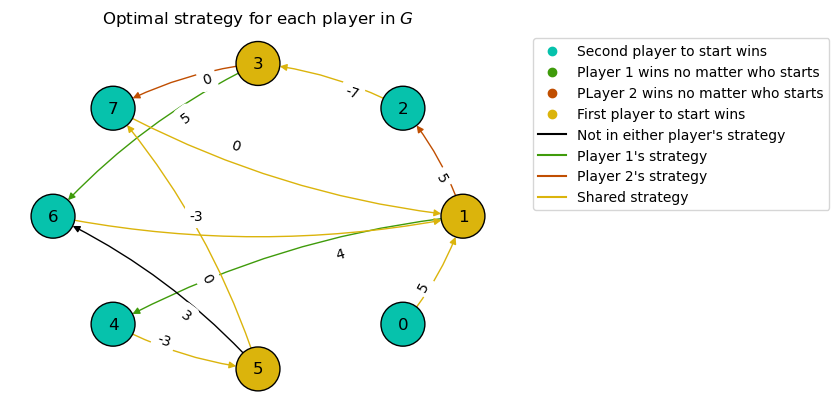
\includegraphics[width= \textwidth]{Figures/OptimalPlayNetworkx.png}
	\caption{Generated visualisation for a Mean Payoff Game with the optimal strategies}
\end{figure}
\FloatBarrier
\subsubsection{games}
This module defines the core functionalities related to mean payoff games.
\newline It also defines the methods to read/write Mean Payoff Graphs. It uses the weighted edgelist format, and supports compression.  
\begin{figure}[H]
	\centering
	\begin{tikzpicture}
		\small
		\begin{package} {networkx}
			\begin{class}{DiGraph}{0,2.5cm}
			\attribute{\dots}
			\operation{\dots}
			\end{class}
		\end{package}
		\begin{package}{ games }
			\begin{class}[text width=12cm]{MeanPayoffGraph}{0,0}
				\inherit{DiGraph}
				\attribute {+ weights\_matrix: Matrix}
				\attribute {+ adjacency\_matrix: Matrix}
				\attribute {+ tensor\_representation: Tensor[3]}
				\operation{+ closure() : MeanPayoffGraph}
				\operation{+ dual() : MeanPayoffGraph}
				\operation {+ as\_bipartite() : MeanPayoffGraph}
				\operation {+ as\_min\_max\_system() : MinMaxSystem}
			\end{class}
			
			\begin{interface}[text width=8.5cm]{Strategy}{0,-5cm}
				\operation{+ \_\_init\_\_(G : MeanPayoffGraph, player : bool)}
				\operation[0]{+ call(vertex : int) : int}
			\end{interface}
			
			\begin{class}[text width=3.5cm]{PositionalStrategy}{-2cm,-8cm}
				\inherit{Strategy}
				\operation[0]{+ call(vertex)}
			\end{class}
			
			\begin{class}[text width=3.5cm]{GreedyStrategy}{-6cm,-8cm}
								\inherit{Strategy}
				\operation[0]{+ call(vertex)}
			\end{class}
			\begin{class}[text width=3.5cm]{EpsGreedyStrategy}{2cm,-8cm}
								\inherit{Strategy}
				\operation[0]{+ call(vertex)}
			\end{class}
			
			\begin{class}[text width=3.5cm]{FractionalStrategy}{6cm,-8cm}
								\inherit{Strategy}
				\operation[0]{+ call(vertex)}
			\end{class}
			
			\begin{class}[text width= 12cm]{Functions}{0,-10cm}
				\operation {@ winning\_everywhere() : bool}
				\operation {@ winning\_somewhere() : bool}
				\operation{@ mpg\_from\_digraph(G : nx.Digraph) : MeanPayoffGraph}
				\operation{@ optimal\_strategy\_pair(G : MeanPayoffGraph) : Tuple[Strategy,Strategy]}
				\operation{@ counter\_strategy(G : MeanPayoffGraph, psi: PositionalStrategy, source : int, player : bool) : Strategy}
				\operation{@ mean\_payoff(G: MeanPayoffGraph, source: int, psi1 : PositionalStrategy, psi2 : PositionalStrategy, turn : bool) : float}
				\operation{@ mean\_payoffs(G: MeanPayoffGraph, psi1 : PositionalStrategy, psi2 : PositionalStrategy) : Matrix}
				\operation{@ winner(G: MeanPayoffGraph, source: int, psi1 : PositionalStrategy, psi2 : PositionalStrategy, turn : bool) : bool}
				\operation{@ winners(G: MeanPayoffGraph, psi1 : PositionalStrategy, psi2 : PositionalStrategy) : Matrix}
			\end{class}
		
		\end{package}
	\end{tikzpicture}
	\caption{\textbf{games} module}
\end{figure}
\FloatBarrier
\subsubsection{ml}
This module defines the required layers, blocks, and model architectures to do machine learning on Mean Payoff Games. This is detailed in chapter \ref{section:ModelDesign}.
\subsubsection{gnn}
This module defines the basic functionalities of graph neural networks \cite{GNN} that are required for our models.

\subsubsection{rl}
This module defines the required functions to do reinforcement learning on Mean Payoff Games\footnote{The current version of this module only supports Mean Payoff Games where at least one player has a fixed strategy.}.

\subsubsection{sp}
This module defines a basic AlphaZero based agent to learn the game.
\subsubsection{wrapper}
This module contains a binding to the C++ implementation of time-critical methods for mean payoff games.
\newline We will give details about this wrapper in the next section.
\subsection{mpgcpp}
This library contains the 
\begin{figure}[H]
	\centering
	\begin{tikzpicture}
		
		\begin{package}{ mpg }
			\begin{class}[text width=3cm]{csp}{0,0}
			\end{class}
			
			\begin{class}[text width=3cm]{games}{4,0}			
			\end{class}
			
			\begin{class}[text width=3cm]{mpgio}{8,0}
			\end{class}
		\end{package}
	\end{tikzpicture}
	\caption{\textbf{mpgcpp} library}
\end{figure}
\subsubsection{csp}
This module contains the constraint satisfaction methods used to solve Mean Payoff Games. 
\subsubsection{games}
This module defines the core functionalities related to mean payoff games.
\begin{figure}[H]
	\centering
	\begin{tikzpicture}
		\small
		\begin{package}{games}
			\begin{abstractclass}[text width=6cm]{MeanPayoffGraphBase}{0,5.5cm}
			\attribute{edges}
			\attribute{dual\_graph}
			\operation[0]{\# add\_edge\_impl(source, target, weight)}
			\operation[0]{\# set\_dual(dual)}
			\operation[0]{+ get\_weight(src, dest)}
			\operation{+ get\_weights()}
			\operation{+ count\_nodes() : int}
			\operation{+ get\_edges() : Edges}
			\end{abstractclass}
			\begin{class}[text width=3.5cm]{VectorMPG}{-6cm,4cm}
				\inherit{MeanPayoffGraphBase}
			\end{class}
			
			\begin{class}[text width=3.5cm]{MatrixMPG}{-6cm,0}
				\inherit{MeanPayoffGraphBase}
			\end{class}
			
			\begin{class}[text width=3.5cm]{HashMapMPG}{6cm,4cm}
				\inherit{MeanPayoffGraphBase}
			\end{class}
			
			\begin{class}[text width=3.5cm]{TreeMapMPG}{6cm,0}
				\inherit{MeanPayoffGraphBase}
			\end{class}
			
			\begin{class}[text width=3.5cm]{DualMPG}{0cm,0cm}
				\inherit{MeanPayoffGraphBase}
			\end{class}
			
			
			\draw[umlcd style,-diamond,fill opacity=100] (DualMPG) to [bend right=12]  (MeanPayoffGraphBase); 
			%\draw[umlcd style,triangle,fill opacity=100] (DualMPG) to [bend right=-12]  (MeanPayoffGraphBase); 
		
			
			\begin{interface}[text width=7.5cm]{Strategy}{0,-2cm}
				\operation{+ \_\_init\_\_(G : MeanPayoffGraph, player : bool)}
				\operation[0]{+ call(vertex : int) : int}
			\end{interface}
			
			\begin{class}[text width=3.5cm]{PositionalStrategy}{-6cm,-5cm}
				\inherit{Strategy}
				\operation[0]{+ call(vertex)}
			\end{class}
			
			\begin{class}[text width=3.5cm]{GreedyStrategy}{-2cm,-5cm}
				\inherit{Strategy}
				\operation[0]{+ call(vertex)}
			\end{class}
			\begin{class}[text width=3.5cm]{EpsGreedyStrategy}{2cm,-5cm}
				\inherit{Strategy}
				\operation[0]{+ call(vertex)}
			\end{class}
			
			\begin{class}[text width=3.5cm]{FractionalStrategy}{6cm,-5cm}
				\inherit{Strategy}
				\operation[0]{+ call(vertex)}
			\end{class}
			
			\begin{class}[text width= 12cm]{Functions}{0,-7cm}
				\operation {@ winning\_everywhere() : bool}
				\operation {@ winning\_somewhere() : bool}
				\operation{@ mpg\_from\_digraph(G : nx.Digraph) : MeanPayoffGraph}
				\operation{@ optimal\_strategy\_pair(G : MeanPayoffGraph) : Tuple[Strategy,Strategy]}
				\operation{@ counter\_strategy(G : MeanPayoffGraph, psi: PositionalStrategy, source : int, player : bool) : Strategy}
				\operation{@ mean\_payoff(G: MeanPayoffGraph, source: int, psi1 : PositionalStrategy, psi2 : PositionalStrategy, turn : bool) : float}
				\operation{@ mean\_payoffs(G: MeanPayoffGraph, psi1 : PositionalStrategy, psi2 : PositionalStrategy) : Matrix}
				\operation{@ winner(G: MeanPayoffGraph, source: int, psi1 : PositionalStrategy, psi2 : PositionalStrategy, turn : bool) : bool}
				\operation{@ winners(G: MeanPayoffGraph, psi1 : PositionalStrategy, psi2 : PositionalStrategy) : Matrix}
			\end{class}
			
		\end{package}
	\end{tikzpicture}
	\caption{\textbf{games} module}
\end{figure}

\subsubsection{mpgio}
Unlike \textbf{mpg}, which has support for mean payoff graph I/O from files via \textbf{NetworkX}. In the C++ library, we have to implement this functionalities from scratch. We used standard I/O utilities with \textbf{boost} to interact with compressed streams conforming to the format used by \textbf{mpg}.
\subsection{Environment}
\subsection{Testing}
\subsection{Structure}

\chapter{Dataset Generation}
\label{section:Dataset}

\section{Introduction}
\section{Analysis}
Generating a Mean Payoff Game can be decomposed into two subsequent objectives.
\begin{enumerate}
	\item Generate the Graph itself.
	\item Generate the Weights
\end{enumerate}


\section{Graph Distributions}
There are many well studied graph distributions in the litterature. \newline
One of the most explored ones are the $\mathcal{G}(n,p)$ and $\mathcal{G}(n,m)$ families.
\subsection{$\mathcal{G}(n,p)$ Family}
For $n\in\mathbb{N},p\in[0,1],$ a graph $G$ is said to follow a $\mathcal{G}(n,p)$ distribution if $\lvert V \rvert=n$ and:
$$
\forall e\in \mathscr{E}, \quad \mathscr{P}(s\in \mathcal{E})=p
$$
Where $\mathscr{E}$ is a set of valid edges. 

\subsection{$\mathcal{G}(n,m)$ Family}
For $n\in\mathbb{N},m\in\mathbb{N},$ a graph $G$ is said to follow a $\mathcal{G}(n,m)$ distribution if $\lvert V \rvert=n,\lvert  E \rvert=m$ and the edges $e_1,\dots,e_m$ were drawn from a set of valid edges $\mathscr{E}.$
\subsection{Valid edges}
The set of valid edges $\mathscr{E}$ is the set defining the potential edges of the graph. It is equal to:
\begin{enumerate}
	\item $V\times V$ for directed graphs with loops 
	\item $(V\times V)\setminus V\odot V$ for directed graphs without loops
	\item The set of subsets of size $2$ of $V$ denoted $\mathscr{P}_2(V)$ for undirected graphs with loops.
	\item The set of subsets of size $2$ of $V$ denoted $\mathscr{P}_2(V)$ for undirected graphs with loops.
\end{enumerate}
\subsection{$\mathcal{D}(n,p)$ Graph Construction}

\subsubsection{Naive Method}
The definition of $\mathcal{D}(n,p)$ gives a straightforward construction. \newline
This is achieved by flipping a coin\footnote{The coin is potentially biased with a probability of obtaining head equal to $p\in [0,1]$} for each pair of node $(u,v)\in V^2$, we add an edge if we get a Head. 
\newline This is implemented in the following algorithm:
\begin{algorithm}
	\caption{$\mathcal{D}(n,p)$ Graph Generation}\label{alg:Dnp_Naive}
	\begin{algorithmic}
		\Require $n\in\mathbb{N}^*$ the size of the graph
		\Require $p\in\mathbb{N}^*$ the edge probability 
		\Ensure $G\sim \mathcal{D}(n,p)$  
		\State $A:(u,v)\in V\times V\rightarrow 0$
		\For{ $u\in V$} 
		\For { $v \in V$ }
		\State Generate $X\sim \mathcal{B}(p)$
		\Comment{$\mathcal{B}(p)$ is the bernoulli distribution}
		\State $A(u,v)\leftarrow X$
		\EndFor
		\EndFor
		\State \Return $G\leftarrow \texttt{GraphFromAdjacencyMatrix}(A)$
	\end{algorithmic}
\end{algorithm}
\FloatBarrier
The complexity\footnote{We assume the cost of generating a Bernoulli random variable as $\mathcal{O}(1)$} of the following algorithm is $\mathcal{O}(n^2).$
\subsubsection{Optimized Method}
Instead of iterating over all possible pair of nodes. For each vertex $v\in V$:
\begin{itemize}
	\item We can sample a number $d$ from the outgoing degree distribution\footnote{Or the ingoing degree distribution, they are in fact equal.}
	\item We then choose $d$ numbers uniformly without replacement from an indexable representation of $V$
\end{itemize}
The following algorithm implements the optimized method:
\begin{algorithm}
	\caption{$\mathcal{D}(n,p)$ Graph Generation Optimisation}\label{alg:Dnp_Fast}
	\begin{algorithmic}
		\Require $n\in\mathbb{N}^*$ the size of the graph
		\Require $p\in\mathbb{N}^*$ the edge probability 
		\Ensure $G\sim \mathcal{D}(n,p)$  
		\State $A:u\in V\rightarrow \varnothing$
		\For{ $u\in V$} 
		\State Generate $d\sim \mathcal{B}(n,p)$
		\Comment{$d$ represents the degree, $\mathcal{B}(n,p)$ is the binomial distribution}
		\State $A(u)\leftarrow \choice(V,d)$
		\EndFor
		\State \Return $G\leftarrow \texttt{GraphFromAdjacencyList}(A)$
	\end{algorithmic}
\end{algorithm}
\FloatBarrier
Now, let $C(a,b)$ be the cost of choice function. 
\newline The expected complexity of this algorithm as a function of $n=\lvert \VertexSet \rvert$ and the degrees $d_1,\dots,d_n$ is:
\begin{align}
	\label{eqn:DnpBigO}
	\tilde{\mathcal{O}}\left(\sum_{i=1}^n1+\mathbb{E}[C(n,d_i)]\right) &= 	\tilde{\mathcal{O}}\left(n+\sum_{i=1}^n\mathbb{E}[C(n,d_i)]\right) 
\end{align}
We will show on the next section what choice function should we use.
\subsection{Choice Function}
\subsubsection{First Proposition}
We propose here a simple choice algorithm, but it is still efficient for our use case.
\newline It works simply by drawing without replacement, but we ignore duplicate elements. This is implemented as follow
\begin{algorithm}
	\caption{$\mathcal{D}(n,p)$ Choice without replacement}\label{alg:Choice}
	\begin{algorithmic}
		\Require $S$ a list
		\Require $m\in\{0,\dots \lvert S \rvert\}$ the number of chosen elements
		\Ensure $H$ a set of size $m$ containing uniformly drawn elements without replacement. 
		\State $H\leftarrow \varnothing$
		\While{$\lvert H \rvert < m$}
			\State Generate $v\sim \mathcal{U}(S)$ 
			\Comment{Where $\mathcal{U}(S)$ is the uniform distribution over $S$}
			\State $H\leftarrow H \cup \{v\}$
		\EndWhile
		\State \Return $H$
	\end{algorithmic}
\end{algorithm}
\FloatBarrier
To estimate the cost of this algorithm, we will use probabilistic reasoning.
\newline Let $X_{n,m}=C(n,m)$ the running time of an execution of algorithm \ref{alg:Choice} in a set $S$ of size $n$, with $m$ elements to be chosen.
We have:
\begin{align*}
	X_{n,0} & \ \text{is deterministic}\\
	X_{n,0}&=\mathcal{O}(1) \\
	\mathbb{E}[X_{n,m}]&=1+\frac{1}{n}\sum_{k=0}^{n-1} \mathbb{E}[X_{n,m} \mid \text{The last drawn number is}\ k] \\
	&=1+\frac{1}{n}\sum_{k=0}^{m-2} \mathbb{E}[X_{n,m}]+\frac{1}{n}\sum_{k=m-1}^{n-1} \mathbb{E}[X_{n,m-1}] \\
	&= 1+\frac{m-1}{n}\mathbb{E}[X_{n,m}]+\frac{n-m+1}{n}\mathbb{E}[X_{n,m-1}]
\end{align*}
Now we arrived at a recurrent formula. We will simplify it as shown below:
\begin{align*}
\frac{n-m+1}{n}\mathbb{E}[X_{n,m}]&=\frac{n-m+1}{n}\mathbb{E}[X_{n,m-1}] +1\\
\implies \mathbb{E}[X_{n,m}]&=\frac{n-m+1}{n-m+1}\mathbb{E}[X_{n,m-1}]+\frac{n}{n-m+1}\\
&=\mathbb{E}[X_{n,m-1}]+\frac{n}{n-m+1} \\
&=\sum_{k=1}^m\frac{n}{n-k+1}+\mathcal{O}(1)\\
&=\sum_{k=0}^{m-1}\frac{n}{n-k}+\mathcal{O}(1) \\
&=n\sum_{k=n-m+1}^n\frac{1}{k}+\mathcal{O}(1)\\
&=n(H_n-H_{n-m})+\mathcal{O}(1)
\end{align*}
Here $(H)_{n\in\mathbb{N}^*}$ is the harmonic series, and we define $H_0=0.$
\subsubsection{Complexity}
%Prooof!!!
The expected complexity of algorithm \ref{alg:Choice} depends on both $n$ and $m$:
\begin{itemize}
	\item If $m=kn+o(n)$ with $k\in\mathopen]0,1\mathclose[$, then it is $\tilde{\mathcal{O}}(m).$
	\item If $m=n-o(n)$, It is\footnote{Here we use the minus sign to emphasize that $m\le n$} $\tilde{\mathcal{O}}(m\log m).$ 
\end{itemize}
To prove this result, we use a well-known asymptotic approximation of the Harmonic series\footnote{This asymptotic approximation can be proven using the Euler–Maclaurin formula} \cite[Section~1.2.11.2]{ArtComputerProgramming}:
$$
H_n=\ln n+\gamma -\frac{1}{2n}+\mathcal{O}\left(\frac{1}{n^2}\right)
$$
We can prove this claim as follow for $m=km+o(m),k\in \mathopen[0,1\mathclose[$:
\begin{align}
	\mathbb{E}[C(n,m)]&=-n\ln \left(1-\frac{m}{n}\right) -\frac{1}{2}\left(1-\frac{n}{n-m}\right)+\mathcal{O}\left(\frac{1}{n}\right) \nonumber \\
&=-n\ln (1-k+o(1))+\frac{1}{n}(1-\tfrac{1}{1-k+o(1)})+\mathcal{O}(\tfrac{1}{n}) \label{eqn:ChoiceBigO} \\
&=\mathcal{O}(m) \nonumber
\end{align}
For $m=n-o(n),$ we prove it by noting that:
\begin{align*}
\mathbb{E}[C(n,m)]&\le\mathbb{E}[C(n,n)]= \mathcal{O} (nH_n) =\mathcal{O}(m\log m)
\end{align*}

\subsubsection{Refinement}
If $m$ tends to $n,$ it is more hard to select $m$ elements from a set of size $n$ without replacement. This explains the extra logarithmic factor.
\newline In that case, we can instead focus on the dual problem: ``Find the $n-m$ elements that will not be selected". This can be calculated in $\mathcal{O}(n-m).$
\newline Once we find the elements that will not be selected, their set complement are exactly the $m$ elements that will be selected. This new algorithm is guaranteed to be $\mathcal{O}(m)$ irrespective of $n$ and $m$
\begin{algorithm}
	\caption{Fine tuned $\mathcal{D}(n,p)$ Choice without replacement }\label{alg:ChoiceFineTuned}
	\begin{algorithmic}
		\Require $S$ a list
		\Require $m\in\{0,\dots \lvert S \rvert\}$ the number of chosen elements
		\Require $\choice$ The choice function defined on algorithm \ref{alg:Choice}
		\Require $\tau$ a fine tuned threshold. We will use $\tau=\frac{1}{2}$ for all practical purposes.
		\Ensure $H$ a set of size $m$ containing uniformly drawn elements without replacement. 
		\If {$\frac{m}{\lvert S \rvert} \le \tau$}
			\State $H\leftarrow \choice(V,n)$
		\Else
			\State $H\leftarrow S\setminus \choice(S,n-m)$
		\EndIf
		\State \Return $H$
	\end{algorithmic}
\end{algorithm}
\FloatBarrier
Also, an important point is that by combining the analysis of all possible cases, we can extract a constant factor that is independent\footnote{The independence can be proven by taking the supremum of the right-hand side of equation \eqref{eqn:ChoiceBigO} over $[0,\tau]$, and the fact that $\tau$ is fixed.} of $n.$ So that the Big-O bound is only a dependent on $m$.
\subsection{Complexity of Optimised $\mathcal{D}(n,p)$ Graph Construction}
Now, using algorithm \ref{alg:ChoiceFineTuned} as the choice algorithm, we can further simplify equation \eqref{eqn:DnpBigO} as a function of only $n=\lvert \VertexSet\rvert$ and $m=\lvert \EdgeSet\rvert.$
\newline This proves that $\Dnp{n}{p}$ construction can be achieved in expected linear time:
\begin{align*}
	\tilde{\mathcal{O}}\left(n+\sum_{i=1}^n\mathbb{E}[C(n,d_i)]\right)  &= \tilde{\mathcal{O}}\left(n+\sum_{i=1}^nd_i\right) \\
	&=\tilde{\mathcal{O}}\left(n+m\right)
\end{align*}

\subsection{$\mathcal{D}(n,m)$ Construction}
To construct a random $\mathcal{D}(n,m)$ graph, we only have to select $m$ uniformly random elements from the set $V\times V.$
\newline We will use algorithm \ref{alg:ChoiceFineTuned} for this purpose\footnote{It is essential that the list $V\times V$ be lazy loaded. In particular, each element will only be loaded when it is indexed. This is essential to reduce the complexity. Otherwise, we will be stuck in an $\mathcal{O}(n^2)$ algorithm.}:
\begin{algorithm}
	\caption{Fine tuned $\mathcal{D}(n,p)$ Choice without replacement }\label{Dnm} 
	\begin{algorithmic}
		\Require $n\in\mathbb{N}^*$
		\Require $m\in\{0,\dots,n^2\}$ the number of chosen elements
		\Ensure $G\sim \mathcal{D}(n,m)$
		\State $E\leftarrow \choice(\text{Lazy}(V)\times \text{Lazy}(V),m)$ \Comment{We only need the $m$ elements on-demand.}
		\State \Return $G\leftarrow \text{GraphFromEdges}(E)$\Comment{This justifies using \text{Lazy}}
	\end{algorithmic}
\end{algorithm}
\FloatBarrier
Here $\text{Lazy}(V)\times \text{Lazy}(V)$ is a lazy implementation of cartesian product that supports bijective indexing\footnote{Indexing is required for uniform sampling} over $\{0,\dots,n^2-1\}.$
\newline The complexity of this construction is: $
\tilde{\mathcal{O}}(m)
$ 

\section{Sinkless Conditionning}
Sampling from a graph distribution may lead to graphs that have at least one sink. 
\newline These graphs are problematic as Mean Payoff Graphs are exactly the sinkless graphs.
\newline To migitate this, we will impose a conditionning on both distribution that will gives a guaranteed Mean Payoff Graph.
\newline We will explore such conditionning both distribution:
\begin{itemize}
	\item $\mathcal{G}^S(n,p):$ This is the distribution of graphs following $\mathcal{G}(n,p)$ with the requirement that they do not have a sink.
	\item $\mathcal{G}^S(n,m):$ This is the distribution of graphs following $\mathcal{G}(n,m)$ with the requirement that they do not have a sink.
\end{itemize}
\subsection{Repeating Construction}
\subsubsection{Algorithm}
This method is very intuitive. It will repeat the sampling until getting the desired graph. \newline The following is an implemention of the repeating construction.
\begin{algorithm}
	\caption{Fine tuned $\mathcal{D}(n,p)$ Choice without replacement }\label{alg:RepeatingConstruction}
	\begin{algorithmic}
		\Require $n\in\mathbb{N}^*$
		\Require $m\in\{0,\dots \lvert S \rvert\}$ the number of chosen elements
		\Require $\choice$ The choice function defined on algorithm \ref{alg:Choice}
		\Require Threshold $\tau$
		\Ensure $H$ a set of size $m$ containing uniformly drawn elements without replacement. 
		\If {$\frac{m}{\lvert S \rvert} \le \tau$}
		\State $H\leftarrow \choice(V,n)$
		\Else
		\State $H\leftarrow V\setminus \choice(S,n-m)$
		\EndIf
		\State \Return $H$
	\end{algorithmic}
\end{algorithm}

\subsubsection{Analysis}
We will analyse the runtime of generating a $\mathcal{G}^S(n,p).$
\newline We expect a similar runtime for $\mathcal{G}^S(n,m)$ due to the similarity between $\mathcal{G}(n,m)$ and $\mathcal{G}(n,p).$ 
\newline Let $F(n)$


\section{Weights Distribution}
\subsection{Construction}
Once the graph is constructed. We only have to generate the weights. \newline
This will be done by creating a random weight function:
$$
W(u,v):(u,v)\rightarrow W_{u,v}
$$
Here $W_{u,v}$ will be a sequence of real random variables. \newline
In our case, we set $(W_{u,v})_{(u,v)\in E}$ to be independent and identically distributed over a real distribution $\mathcal{W}.$ 


\section{Proposed MPG Distribution}
\subsection{Desired Properties of Mean Payoff Game Distributions}
\subsubsection{Fairness in the Limit}
This is essential, as we intend to generate a sequence of Mean Payoff Games that do not favour statistically a certain player, in the sense that, if we generate sufficient independent and identically distributed Mean Payoff Games $G_1,\dots,G_n$, we expect the following:
$$
\lim_{n\rightarrow +\infty} \left\lvert \mathtt{R}_{\Max}(G_1,\dots,G_n)-\mathtt{R}_{\Min}(G_1,\dots,G_n)\right \rvert = 0
$$
Where $\mathtt{R}$ is defined as follow:
$$
\mathtt{R}_{\text{Op}}(G_1,\dots,G_n)=\frac{1}{n}\sum_{i=1}^n\mathscr{P}(\text{Op wins} \ G_i\ \text{assuming optimal strategies})
$$
\subsubsection{Symmetric}
A real distribution is said to be symmetric if:
$$
\forall [a,b]\in \mathbb{R},X\sim \mathcal{W},\quad \mathscr{P}(X\in [a,b]) = \mathscr{P}(X\in [-b,-a])
$$
We will define a symmetric Mean Payoff Game distribution as a distribution of Mean Payoff Game whose weights are independent and identically distributed on a symmetric real distribution.
This property is stronger than Fairness in the Limit, as it implies that:
$$
\mathscr{P}(\text{Max wins} \ G\ \text{assuming optimal strategies}) = \mathscr{P}(\text{Min wins} \ G\ \text{assuming optimal strategies})
$$
We will require a Symmetric Mean Payoff Game as we do not want a player to have an inherit advantage other the other one\footnote{Other than the first move.}
\subsection{Implemented Distributions}
The following table resumes the implemented distributions:
\begin{table}[h]
	\small
	\begin{tabularx}{\textwidth}{| X | X | X |}
		\hline
		
		Distribution Family & Parameters & Type  \\
		\hline
		$\mathcal{D}(n,p)$ & \vspace{-5mm}
		\begin{itemize}
			  \setlength\itemsep{0em}
			\item $n:$ Graph size
			\item $p:$ Edge probability
		\end{itemize} & Graph distribution \\
		\hline
		$\mathcal{D}(n,m)$ & 
		\vspace{-5mm}
		\begin{itemize}
			  \setlength\itemsep{0em}
			\item $n:$ Graph size
			\item $m:$ Number of edges
		\end{itemize} & Graph distrbiution  \\
		\hline
		$\mathcal{U}_{\text{discrete}}(-r,r)$ &
		\vspace{-5mm}
		\begin{itemize}
			  \setlength\itemsep{0em}
			\item $r:$ The radius of the support
		\end{itemize}
		 &  Weight distribution\\
		\hline
		$\mathcal{U}(-r,r)$ &\vspace{-5mm}
		\begin{itemize}
			  \setlength\itemsep{0em}
			\item $r:$ The radius of the support
		\end{itemize} & Weight distribution \\
		\hline
		$\mathcal{N}(0,\sigma)$ &
		\vspace{-5mm}
		\begin{itemize}
			  \setlength\itemsep{0em}
			\item $\sigma:$ The standard deviation
		\end{itemize} & Weight distribution\\ 
		\hline 
		
	\end{tabularx}
	\caption{Le tableau d'avancement des BNNs
	\label{table:Distributions}}
\end{table}
\FloatBarrier
Also, to generate the initial state, we have defaulted to:
\begin{itemize}
	\item The uniform distribution over the vertices to generate the starting vertex
	\item The bernoulli distribution to generate the starting player.
\end{itemize}
With all that said, distributions are fair in the limit and are symmetric, provided that the underlying graph distribution and weight distribution are chosen from the table \ref{table:Distributions}.

\section{MPG Generation}
\label{section:MPG:Generation}
\subsection{Distribution}
\begin{itemize}
	\item Each generated graph will follow a distribution $\mathcal{G}(n,p(n))$  for some $n\in\mathbb{N}^*$
	\item The weights will follow the discrete uniform distribution $\mathcal{D}(-1000,1000)$

\end{itemize}

We will generate two kinds of datasets, depending on the nature of the graph

\subsection{Dense Graphs}
\begin{itemize}
	\item Let $\mathcal{P}=\{0.1,0.2,0.3,0.5,0.7,0.8,0.9,1\}$
	\item $\mathcal{N}=\{10,20,30,40,50,60,70,80,90,100,110,120,130,140,150,200,250,300,400,500\}$
	\item For each $(n,p)\in \mathcal{N}\times \mathcal{P},$ we will generate $K=1000$ observations $G^{n,p}_1,\dots,G^{n,p}_{K} \sim \mathcal{G}(n,p)$ 
\end{itemize} 

The total number of examples is:
$$
K\times\lvert \mathcal{N} \rvert \times \lvert \mathcal{P}\rvert=160000
$$
The generation was done on a `haswell64` partition with 24 cores. and it took 02:12:38 hours.

\section{Annotation}
\subsection{Approach}
We used the CSP algorithm $\ref{alg:AC3Optimized}$ to annotate the dataset, potentially augmented with some heuristics. 
\newline We implemented a program that takes the path of the dataset, and solves the Mean Payoff Games one by one.
\newline To maximize efficiency, the program launches many solver threads, with each one independently working on a single file, and the results are accumulated using a ConcurrentQueue.
\subsection{Target Values}
The solver will calculate the following targets:
\begin{itemize}
	\item The optimal pair of strategies
	\item The mean payoffs for each starting position, turn.
	\item The winners for each starting position, turn.
\end{itemize}
Also, some additional metadata are generated for analysis:
\begin{itemize}
	\item \texttt{dataset}: The name of the whole dataset
	\item \texttt{graph}: The name of the graph.
	\item \texttt{status}: The solver's status on the given graph. In particular, whether it succeeded to solve the instance or not\footnote{We expect that the solver may crash due to several reasons (corrupted file, out of memory, etc\dots). For that we made additional effort for exception handling, so that an error for a single instance does not propagate to the whole program.}. Equal to ``OK" if the execution is successful.
	\item \texttt{running\_time}: The time needed to solve the instance.

\end{itemize}

\subsection{Heuristics}
To accelerate the annotation of the two datasets, we had to apply some heuristics to the algorithm. We made essentially two kinds of heuristics.
\subsubsection{Linear Bound Heuristic}
This is the heuristic based on the view that for almost all solutions of a Ternary Max Atom system extracted from our generated random games, either:
\begin{itemize}
	\item All variables are infinite: 
	$$
	X(u)=-\infty \quad \forall u\in V$$
	\item The diameter of assignments is in the order of $\lVert W\rVert_{\infty}$
	$$
	\Delta X = \sup_{u\in V}X(u)-\inf_{u\in V,X(u)>-\infty}X(u)= \mathcal{O}(\lVert W\rVert_{\infty})$$
\end{itemize}
This heuristic suggests a much tighter search space to the worst case $\lVert W \rVert_{1}$ one. Going further, with uniform random weights:
$$
\lVert W \rVert_{1}=\mathcal{O}\left(\lvert E \rvert \times \lVert W \rVert_{\infty}\right)
$$
We believe this heuristic arises due to the random property of graphs, because in general, one can build an infinite family of ternary max atom systems that violate this heuristic. \newline In fact, going further, one can build ternary max atom systems were the $\lVert W \rVert_{1}$ estimation is tight.
%Example of such system:
% Linear chain of constraints 

To generating the dataset, we applied this heuristic with $\Delta X=4\lVert W\rVert_{\infty}$
$$
D = \{-\infty,-2 \lVert W\rVert_{\infty},,-2 \lVert W\rVert_{\infty}+1 ,\dots ,2\lVert W\rVert_{\infty} \}
$$

\begin{figure}[H]
	\centering
	\begin{tikzpicture}[node distance={20mm}, thick, main/.style = {draw, circle}]
		\node[main] (1) {$0$}; 
		\node[main] (2) [right of =1] {$1$}; 
		\node[main] (3) [right of =2] {$2$}; 
		\node[main] (4) [right of =3] {$3$}; 
		\node[main] (5) [right of =4] {$\dots$}; 
		\node[main] (6) [right of =5] {$n-1$}; 
		\node[main] (7) [right of =6] {$n$}; 
		\draw[->] (1) -- node[midway, above right, sloped, pos=0.3] {-5} (2);
		\draw[->] (2) -- node[midway, above, sloped, pos=0.5]{6} (3);
		\draw[->] (3) -- node[midway, above, sloped, pos=0.5] {-8} (4);
		\draw[->] (4) -- node[midway, above, sloped, pos=0.5] {-5}(5);
		\draw[->] (5) -- node[midway, above, sloped, pos=0.5] {7}(6);
		\draw[->] (6) -- node[midway, above, sloped, pos=0.5] {2}(7);
	\end{tikzpicture} 
	\caption{A counter example of the Linear Bound heuristic}
\end{figure}

\subsubsection{Early Stopping}
If after any iteration of arc consistency, $\max_{x\in V}\nu(x) < \sup D.$ Then, $\nu(t)$ will converge to $-\infty$ for all $t.$ 
\newline Thus, we stop the algorithm and sets $\nu(t)\leftarrow -\infty,\quad \forall t$
\begin{proof} 
suppose that in fact there is an assignment with: 
$$
-\infty < \max_{u\in V}\nu(u) < \sup D$$
We will take the $u$ with the biggest such $\nu(u).$  
\newline Now our system is a tropical max atom system, which means translations are also a polymorphism of this system, so for any assignment $\nu:V\rightarrow\mathbb{Z},\ X+t$ is also an assignment $\forall t\in \mathbb{Z}.$ With that, $\nu+\sup D-\nu(u)$ is also an assignment.
\newline This assignment has the property: $$
\forall s\in V,\quad \nu(s)+\sup D-\nu(u) \in D
$$
Which is a contradiction, as it violates the consistency of arc consistency, and the maximality of the solution with respect to the domain $D$
\end{proof}
  
The efficiency of the Early Stopping heuristic depends on the density of the graph. Empirically, for dense graphs. the analoguous ternary max atom system usually has two kind of assignments:
\begin{enumerate}
	\item Either all variables are finite
	\item Either all variables are $-\infty$
\end{enumerate}
This translates back in a dense Mean Payoff setting, that the winner of the game usually does not depend in the starting position and the starting turn. 
\newline With that, the Early Stopping heuristic will quickly detect the second case, which we believe as the hurdle of the algorithm.
\newline On the other hand, for sparse graphs, we do not have this nice distinction between finite and infinite assignments, and they can overlap, and so will make this heuristic useless in practice.

\subsection{Implementation}
\subsubsection{Algorithm}
We implemented a Mean Payoff Graph solver. It calculates the optimal move for each player in each position. Thus, our implementation gives an exact solution to the optimization problem\footnote{In its current version, It gives a weak optimal strategy for both players $\Max,$ and $\Min.$ The winning condition is $C_2$ }  for Mean Payoff Games.
\newline It works by a transforming a mean payoff game to an equivalent min-max system, then applying two subsequent reductions to a $n$-ary max atom system, then to a ternary max atom system. The solution of the latter is propagated back to mean payoff game to induce an optimal strategy.
\begin{algorithm}
	\caption{Solving a Mean Payoff Graph for all states}\label{alg:MPGSolver}
	\begin{algorithmic}
		\Require $G$ a Mean Payoff Graph
		\Require $D$ the domain of the variables. Can be chosen by heuristics.
		\Ensure $\Phi:V\times P\rightarrow V$ The optimal strategy of each player
		\State $\Phi\leftarrow \varnothing$
		\For {$p\in P$}
		\If {$p$ is Max}
		\State $G'\leftarrow G$
		\Else
		\State $G'\leftarrow \bar{G}$
		\EndIf
		\State $S \leftarrow \displaystyle \transform_{\text{MPG}\rightarrow \text{Min-Max}}(G',D)$ 
		\State $S' \leftarrow \displaystyle \transform_{\text{Min-Max}\rightarrow \text{Max}}(S)$ 
		\State $S'' \leftarrow \displaystyle \transform_{\text{Max}\rightarrow \text{Max}_3}(S')$
		\State $L\leftarrow \inf D$
		\State $R\leftarrow \sup D$
		\State $Q\leftarrow \emptyset$
		\State $\mathcal{V} \leftarrow \text{Variables}(S'')$
		\For {$u\in \mathcal{V}$}
			\State $X(u)\leftarrow R$
			\State $\text{append}(Q,u)$
		\EndFor
		\While {$Q\neq \varnothing}$ 
			\State $X\leftarrow \arcconsistency(S'',X,Q,L)$
		\EndWhile
		\For {$\mathcal{C}\in S''$} \Comment{Iterate over constraints of $S''$}
		\State $\text{OP}\leftarrow \text{Operator}(\mathcal{C})$
		\Comment{Get the operator of $\mathcal{C}.$ Either Max or Min }
		\State $Y$ the right-hand side variables of $\mathcal{C}$
		\State $C$ the right-hand side constants of $\mathcal{C}$
		\State $x$ the left-hand side variable of $\mathcal{C}$
		\State $u\leftarrow \displaystyle \projection_{V\times P\rightarrow V}(x)$ \Comment{Extract the vertex}
		
		\If {$\text{OP}$ is Max}
		\State $y^*,c^*\leftarrow  \displaystyle\argmax_{(y,c)\in \zip(Y,C)}\{X(y)+c\}$ \Comment{Extracts the maximum assignment}
		\State $\Phi(u,p)\leftarrow \displaystyle \projection_{V\times P\rightarrow V}(y^*)$ \Comment{The Strategy is the vertex of the maximum assignment}
		\EndIf
		\EndFor
		\EndFor
		\State \Return $\Phi$
	\end{algorithmic}
\end{algorithm}
\FloatBarrier
Here $\zip(Y,C)$ of lists $Y$ and $C$ is the list $L=[(y_1,c_1),\dots,(y_n,c_n)]$

These transformations were not trivial to find, we had to improve the reductions offered by \cite{MPGMaxAtom}, we also proposed a refinement to arc consistency that works for a ternary max-atom system, that takes advantage of polymorphisms, as well as the symmetries.
\newline This is very technical, and for that, the details are listed in the appendix \ref{appendix:CSP}.
\subsubsection{Complexity Analysis}
For simplicity will suppose that the domain $D$ is finite\footnote{In particular, a finite subset of $\mathbb{Z}$}, our algorithm runs in:
\begin{equation*}
	\mathcal{O}\left((\lvert V\rvert +\lvert E\rvert)^2 \cdot \lvert D\right\rvert)
\end{equation*}
Otherwise, if $D$ is a real domain, the algorithm still converges if $D$ is bounded\footnote{$D\subseteq [a,b]$ for some interval $[a,b]$}, since arc consistency takes a function and produces a smaller one. With that said, we did not produce a complexity estimation, as our work directly relies to the generated graphs that we have discussed in section \ref{section:MPG:Generation}, we recall that their weights are finite.


\subsection{Deployment}
After some experiments, it was very clear that vertical scaling with the number of threads is not sufficient. By analysing the running time of some samples, we estimated the total running time solving both datasets to exceed $30$ days.
\newline As a result of this, we deployed a pipeline of $24$ nodes, each with $24$ threadss working simultaneously on a partition of the dataset.
 
\chapter{Model Design}
\label{section:ModelDesign}

\section{Introduction}

\section{Objectives}
The main objective

\section{Properties}
\label{section:ModelDesign:Properties}
We expect the model $\mathcal{M}$ to verify the following properties:

\subsection{Totality}
\subsubsection{Definition}
A function is total if it is defined in the whole domain.
\newline Also, we will say a model $\mathcal{M}$ is total if it works on all Mean Payoff Games..
\subsubsection{Importance}
This property implies two main characteristics:
\begin{enumerate}
	\item The model works for any Mean Payoff Game whatever the size of $\lvert \VertexSet \rvert.$ This is tricky as most machine learning models act on a batch of data with a fixed shape.
	\item The model works for any Mean Payoff Game whatever the representation is; This is implicitely verified by an encoding of the Mean Payoff Games.
\end{enumerate}

\subsection{Node Agnostic}
This property tells that a model should not use any extra information about the nodes.
\subsubsection{Formalisation}
Let $G_1(V_1,E_1,W_1,s_1),G_2(V_2,E_2,W_2,s_2)$ two isomorphic Mean Payoff Games in the sense that there exists a bijection $\Phi:V_1\rightarrow V_2$ such that:
\begin{align*}
	E_2&=\{(\Phi(u),\Phi(v)),\quad (u,v)\in E_1\}\\
	\forall (u,v)\in E_1,\quad W_2(u,v)&=W_1(\Phi(u),\Phi(v)) \\
	s_2&= \Phi(s_1)
\end{align*}
Then:
$$
\Phi\left(\mathcal{M}(G_1)\right) = \mathcal{M}(G_2)
$$
\subsubsection{Explanation}
The property tells that if two graphs mean payoffs only differ by their node representation, then the results should also only differ by the representation of the nodes.

\subsubsection{Importance}
This property implies that we can simply encode a mean payoff as $G(V,E,W,s)$ as $G'(V',E',W',s')$ with  $V'=\{0,\dot,\lvert V \rvert-1\},$ and $E',W',s'$ defined accordingly.
\newline In fact, the encoding is done implicitely by our model\footnote{While the encoding is done implicitely, the model itself can violate this property. An example of this is a Multi Layer Perceptron. Which lead to different results for different encodings.}.

\begin{figure}[H]
	\begin{subfigure}[b]{0.3\textwidth}
		\begin{tikzpicture}[->,>=stealth',shorten >=1pt,auto,node distance=2cm,
			thick,main node/.style={circle,draw,font=\Large\bfseries}]
			\node[main node, fill=gray!50] (1) {$2$}; 
			\node[main node] (2) [right of =1] {$3$}; 
			\node[main node] (3) [above right of =1] {$0$}; 
			\node[main node] (4) [right of =2] {$1$}; 
			\path (1) edge [bend left] node {1} (3)
			edge [bend right] node [below] {-1} (2)
			(2) edge [bend right] node [above] {1} (1)
			edge [loop below] node {-1} (2)
			(3) edge [bend left] node {-5} (2)
			edge [bend left] node {-2} (4)
			(4) edge node {3} (2);
		\end{tikzpicture} 
	\end{subfigure}
	\hfill
	\begin{subfigure}[b]{0.3\textwidth}
		\begin{tikzpicture}[->,>=stealth',shorten >=1pt,auto,node distance=2cm,
			thick,main node/.style={circle,draw,font=\Large\bfseries}]
			\node[main node, fill=gray!50] (1) {$0$}; 
			\node[main node] (2) [right of =1] {$1$}; 
			\node[main node] (3) [above right of =1] {$2$}; 
			\node[main node] (4) [right of =2] {$3$}; 
			\path (1) edge [bend left] node {1} (3)
			edge [bend right] node [below] {-1} (2)
			(2) edge [bend right] node [above] {1} (1)
			edge [loop below] node {-1} (2)
			(3) edge [bend left] node {-5} (2)
			edge [bend left] node {-2} (4)
			(4) edge node {3} (2);
		\end{tikzpicture}
	\end{subfigure} 
	\hfill
	\begin{subfigure}[b]{0.3\textwidth}
		\begin{tikzpicture}[->,>=stealth',shorten >=1pt,auto,node distance=2cm,
			thick,main node/.style={circle,draw,font=\Large\bfseries}]
			\node[main node, fill=gray!50] (1) {\scriptsize Cat}; 
			\node[main node] (2) [right of =1] {\scriptsize Dog}; 
			\node[main node] (3) [above right of =1] {\small Yak}; 
			\node[main node] (4) [right of =2] {\scriptsize Fox}; 
			\path (1) edge [bend left] node {1} (3)
			edge [bend right] node [below] {-1} (2)
			(2) edge [bend right] node [above] {1} (1)
			edge [loop below] node {-1} (2)
			(3) edge [bend left] node {-5} (2)
			edge [bend left] node {-2} (4)
			(4) edge node {3} (2);
		\end{tikzpicture} 
	\end{subfigure}
	\caption{Three isomorphic Mean Payoff Games}
	\label{fig:NodeAgnostic}
\end{figure}
\FloatBarrier
In the figure \ref{fig:NodeAgnostic}, we have $3$ equivalent Mean Payoff Games.
To illustrate a node agnostic model:
\begin{itemize}
	\item Let $\mathcal{M}$ be a model that predicts for a given Mean Payoff Game, the action to be played at the starting node, and the winner.
	\item Suppose also that $\mathcal{M}(G_1)=(3,\text{Max})$
\end{itemize}
If $\mathcal{M}$ is node agnostic, then:
\begin{align*}
	\mathcal{M}(G_2)&=(1,\text{Max})\\
	\mathcal{M}(G_3)&=(\text{Dog},\text{Max})
\end{align*}
\subsection{Invariance under Positive Scaling}
\label{section:ModelDesign:Properties:Invariance}
This property comes directly from the fact that both the winner and the set of optimal strategies\footnote{Whatever the definition of optimality (Weak, Strong, Payoff).} are invariant under a positive scaling of the weights.
\newline
Now, it is very easy to make augment a model $\mathcal{M}$ into such invariant model $\mathcal{M}'.$ We only do the following:
$$
\mathcal{M}'(E,W,s)=\mathcal{M}'(E,\text{Normalize}(W),s)
$$
Where $\text{Normalize}$ is any endomorphism of weight functions that verify the following constraint:
$$
\forall_{\text{MPG}}G(E,W),\forall ,\quad \text{Normalize}(W)=\frac{W}{H(W)}
$$
With $H:\mathscr{F}(E,\mathbb{R})\rightarrow \mathscr{F}(E,\mathbb{R})$ a function satisfying\footnote{Special care must be when $H$ is $\ge$ instead of $>$}:
\begin{align*}
	\forall s\in\mathbb{R}_+^*,\quad H(sW)&=sH(W) \\
	H(W)&> 0
\end{align*}

\subsubsection{Standard Scaling}
This scaling treats the values of $W$ as samples of random variables, and divides $W$ by an estimate of their variance. 
\begin{align*}
	\text{Normalize}(W)&=\frac{W}{\sqrt{\mathbb{V}[W]}}\\
	\mathbb{V}[W]&=\frac{1}{\lvert E \rvert} \sum_{(u,v)\in E}(W(u,v)-\mathbb{E}[W])^2 \\
	\mathbb{E}[W]&=\frac{1}{\lvert E \rvert}\sum_{(u,v)\in E}W(u,v) 
\end{align*}



\subsubsection{Maximum Scaling}
This scaling reduces the interval of the weights to $[-1,1]$ by dividing by the largest weight in terms of absolute value:
$$
\text{Normalize}(W)=\frac{W}{\lVert W \rVert_{\infty}}
$$
\paragraph{Implementation Notes:}
The weights function is implemented as a matrix $W,$ which is equal to $0$ for $(u,v)\notin E.$ 
\newline It is important to igonre these zeros\footnote{And only these zeros. If $W(u,v)=0$ for $(u,v)\in E$, this term should be accounted.} in both normalisations, otherwise it may lead to biased scaling.

\begin{figure}[H]
	\begin{subfigure}[b]{0.45\textwidth}
		\raggedleft
		\begin{tikzpicture}[->,>=stealth',shorten >=1pt,auto,node distance=2cm,
			thick,main node/.style={circle,draw,font=\Large\bfseries}]
			\node[main node, fill=gray!50] (1) {$2$}; 
			\node[main node] (2) [right of =1] {$3$}; 
			\node[main node] (3) [above right of =1] {$0$}; 
			\node[main node] (4) [right of =2] {$1$}; 
			\path (1) edge [bend left] node {1} (3)
			edge [bend right] node [below] {-1} (2)
			(2) edge [bend right] node [above] {1} (1)
			edge [loop below] node {-1} (2)
			(3) edge [bend left] node {-5} (2)
			edge [bend left] node {-2} (4)
			(4) edge node {3} (2);
		\end{tikzpicture} 
	\end{subfigure}
	\hfill
	\begin{subfigure}[b]{0.45\textwidth}
		\raggedright
		\begin{tikzpicture}[->,>=stealth',shorten >=1pt,auto,node distance=2cm,
			thick,main node/.style={circle,draw,font=\Large\bfseries}]
			\node[main node, fill=gray!50] (1) {$2$}; 
			\node[main node] (2) [right of =1] {$3$}; 
			\node[main node] (3) [above right of =1] {$0$}; 
			\node[main node] (4) [right of =2] {$1$}; 
			\path (1) edge [bend left] node {0.2} (3)
			edge [bend right] node [below] {-0.2} (2)
			(2) edge [bend right] node [above] {0.2} (1)
			edge [loop below] node {-0.2} (2)
			(3) edge [bend left] node {-1} (2)
			edge [bend left] node {-0.4} (4)
			(4) edge node {0.6} (2);
		\end{tikzpicture} 
	\end{subfigure}
	\caption{Mean Payoff Game, with a rescaled version using Maximum normalization}
\end{figure}

\subsection{Permutation Equivariance}
\subsubsection{Definition}
This property states that the model should ouptut the same results for permuted nodes, up to permutation of the results.
\subsubsection{Importance}
While it is a special case of the Node Agnostic property, but it is still important as the encoding of the graphs is done implicitely, and thus Permutation Equivariance is enough to get a Node Agnostic model.
\subsection{Stability under Padding}
\label{section:Model:Properties:Scaling}
\subsubsection{Definition}
\begin{itemize}
	\item Let $G_1(V_1,E_1,W_1,s_1),G_2(V_2,E_2,W_2,s_2)$ be two disjoint Mean Payoff Games, in the sense that $V_1\cap V_2=\varnothing.$
	\item Let $B=(E_3,W_3)$ with $E_3\subseteq V_2\times V_1$ a bridge from $G_2$ to $G_1,$ and $W_3$ is the weight function of $E_3$
\end{itemize}
The padding of $G_1$ by $G_2$ using $B$ as a bridge, denoted as $G_1\overset{B}{\rhd} G_2$ is defined as:
$$
G_1\overset{B}{\rhd} G_2=(V_1\cup V_2,E_1\cup E_2 \cup E_3,W_1\cup W_2 \cup W_3,s_1)
$$
If the bridge $B$ is empty, in the sense that $E_3=\emptyset,$ then we denote we will simplify the notation to $G_1 \rhd G_2.$
\newline 
A model is said to be stable under padding if:
$$
\mathcal{M}(G_1\overset{B}{\rhd} G_2)=\mathcal{M}(G_1)
$$
\subsubsection{Importance}
Deep Learning algorithms generally accept batches of data having a homogeneous shape.
\newline In the other hand, graph input generally has different shapes, and thus are problematic to most learning algorithms.
\newline While we succeeded in experimenting a learning algorithm with a ragged batch\footnote{A batch of inhomogeneous input}, it suffered the following limits:
\begin{itemize}
	\item It greatly limits the choice of potential models. 
	\item The training is not supported by GPU, as some core operations were only implemented in the CPU for ragged batches.
\end{itemize}
For this reasons, we opted to pad the graphs to get homogeneous batches, and this is why the stability under padding is important.
\subsubsection{Removing Unreachable Nodes}
Another major point for this property, is it gives the possibility to remove unreachable nodes without affecting the model's results.
\begin{figure}[H]
	\begin{subfigure}[b]{0.45\textwidth}
		\raggedleft
		\begin{tikzpicture}[->,>=stealth',shorten >=1pt,auto,node distance=2cm,
			thick,main node/.style={circle,draw,font=\Large\bfseries}]
			\node[main node, fill=gray!50] (1) {$2$}; 
			\node[main node] (2) [right of =1] {$3$}; 
			\node[main node] (3) [above right of =1] {$0$}; 
			\node[main node] (4) [right of =2] {$1$}; 
			
			\node[main node, fill=red!50] (7) [below of =2] {$6$}; 
			\node[main node, fill=red!50] (5) [below left of =7] {$4$}; 
			\node[main node, fill=red!50] (6) [below right of =7] {$5$}; 
			\path (1) edge [bend left] node {1} (3)
			edge [bend right] node [below] {-1} (2)
			(2) edge [bend right] node [above] {1} (1)
			edge [loop below] node {-1} (2)
			(3) edge [bend left] node {-5} (2)
			edge [bend left] node {-2} (4)
			(4) edge node {3} (2)
			(5) edge node {-3} (7)
			edge node {-2} (1)
			(6) edge node {5} (5)
			(7) edge node {0} (6)
			edge node {-5} (4);
		\end{tikzpicture} 
	\end{subfigure}
	\hfill
	\begin{subfigure}[b]{0.45\textwidth}
		\raggedright
		\begin{tikzpicture}[->,>=stealth',shorten >=1pt,auto,node distance=2cm,
			thick,main node/.style={circle,draw,font=\Large\bfseries}]
			\node[main node, fill=gray!50] (1) {$2$}; 
			\node[main node] (2) [right of =1] {$3$}; 
			\node[main node] (3) [above right of =1] {$0$}; 
			\node[main node] (4) [right of =2] {$1$}; 
			\path (1) edge [bend left] node {0.2} (3)
			edge [bend right] node [below] {-0.2} (2)
			(2) edge [bend right] node [above] {0.2} (1)
			edge [loop below] node {-0.2} (2)
			(3) edge [bend left] node {-1} (2)
			edge [bend left] node {-0.4} (4)
			(4) edge node {0.6} (2);
		\end{tikzpicture} 
	\end{subfigure}
	\caption{Mean Payoff Game before and after removing unreachable nodes}
	\label{fig:StableUnderPadding}
\end{figure}
\FloatBarrier
Following the example under figure \ref{fig:StableUnderPadding}, if the model $\mathcal{M}$ is stable under padding, then the vertices $\{4,5,6\}$ can be removed without affecting the results.
\newline In fact, this is true as the original mean payoff game can be constructed from the reduced one with a suitable padding.
\section{Considered Models}
While there are many possible predictive models. We considered mainly two families of predictive models.
\subsection{Value based Model}
Such model predicts the evaluation of a certain position.
\newline The evaluation is a function $\mathcal{M}:\VertexSet \times \PlayerSet \rightarrow [-1,1]$ with the following interpretation:
\begin{itemize}
	\item $\mathcal{M}(s,p)=1$ when the model predicts that player $p$ will win the game given the position.
	\item $\mathcal{M}(s,p)=-1$ whens the model predicts that player $p$ will lose the game given the position.
	\item $\mathcal{M}(s,p)=0$ when the model predicts that the position will result in a draw.
\end{itemize}
Now, while such a model can be used to predict the winner. We claim that it is not efficient\footnote{Efficient in the sense that we cannot extract the best strategy from the evaluation in linear time.} to extract the strategy from such model, as the information of winning alone does not directly induce a strategy.
\newline The following figure illustrates an example.
\begin{figure}
	\centering
	\begin{tikzpicture}[->,>=stealth',shorten >=1pt,auto,node distance=4cm,
		thick,main node/.style={circle,draw,font=\Large\bfseries}]
		\node[main node] (5) {$5$};
		\node[main node, fill=gray!50] (1) [below left of =5] {$0$}; 
		\node[main node] (2) [below right of =5] {$1$}; 
		\node[main node] (3) [above right of =5] {$2$}; 
		\node[main node] (4) [above left of =5] {$3$}; 
		\path (1) edge [bend left=12] node {1} (5)
				  edge node {-1} (2)
		(2) edge node {-1} (3)
		edge [bend left=12] node {1} (5)
		(3) 
		edge [bend left=12] node {1} (5)
		edge node {-1} (4)
		(4)
		edge node {-1} (1)
		edge [bend left=12] node {1} (5)
		(5) edge [bend left=12] node {1} (1)
			edge [bend left=12] node {1} (2)
			edge [bend left=12] node {1} (3)
			edge [bend left=12] node {1} (4);
			
	\end{tikzpicture} 
	\caption{An MPG where the first player always wins.}
\end{figure}
\FloatBarrier
\subsection{Strategy based Model}
Such model predicts the strategy for each player.
\newline This is a function $\mathcal{M}:\VertexSet \times \PlayerSet \rightarrow \mathscr{P}(\VertexSet)$ such that:
\begin{align*}
	\forall (u,p)\in \VertexSet \times \PlayerSet, \quad \mathcal{M}(u,p) &\in \Adj u \\
	\forall (u,p) \in \VertexSet \times \PlayerSet,\forall v \in \Adj u, \quad  \mathcal{P}\left(\mathcal{M}(u,p) =v \right)  &\in [0,1] \\ 
\forall (u,p) \in \VertexSet \times \PlayerSet, \quad  \sum_{v\in \Adj u}\mathcal{P}\left(\mathcal{M}(u,p) =v \right) &=1 \\ 
\end{align*}
\section{Building the Model}
Our model follows from well esta../Figures/PreprocessingBlock.pngblished graph neural network architectures, with minor modifications to suit our needs.
\newline It is composed of blocks, each containing a \textbf{Weighted Graph Convolutional Network}.

\subsection{Preprocessing Block}
The preprocessing block is responsible to convert the graph to a format recognizable by the convolutional blocks.
\newline It takes the following steps:
\begin{enumerate}
	\item It takes a batch, add a padding to each graph so that the resulting batch is of homogenous shape.
	\item It adds some random edges to each graph, with some low probability \texttt{random\_connection\_probability}.
	\item It normalizes the weights.
	\item It adds some noise to the weights.
\end{enumerate} 

\subsubsection{Padding Layer}
First of all, we define $H_k$ be the graph of size $k$ in which all the edges are loops with $0$ as a weight. 
\newline Each graph $G^{(i)}=(A^{(i)},W^{(i)})$ in the batch has a size $r_i.$ 
\newline Let $r=\max_i r_i.$ The padding layer adds a potential padding to each graph in the following manner:
\begin{equation*}
	G^{(i)}\leftarrow G^{(i)} \rhd I_{r-r_i}
\end{equation*}
With that, the resulting batch will be of shape $(?,r,r,2)$
\subsubsection{Random Connections}
This layer adds an edge with some probability $p:$
\begin{equation*}
	A^{(i)}\leftarrow A^{(i)} \vee B^{(i)}
\end{equation*}
Where $B^{(i)}$ is a matrix of shape $(r,r)$ whose elements are sampled from the bernoulli distribution $\mathcal{B}(p)$.
\subsubsection{Weights Normalisation}
We want the model to be invariant under positive scaling. To achieve that, we implemented a weights normalization layer conforming to section \ref{section:Model:Properties:Scaling}
\subsubsection{Weights Noise}
For regularization, we implemented a weights noise layer, that adds a small additive noise to the weights, in the following manner:
\begin{equation*}
		W^{(i)}\leftarrow W^{(i)} + N^{(i)} \odot A^{(i)}
\end{equation*}
Where $N^{(i)}$ is the noise matrix. We implemented two kinds of noise:
\begin{itemize}
	\item Uniform noise, where each element of $N^{(i)}$ follows $\mathcal{U}(-r,r)$
	\item Gaussian noise, where each element of $N^{(i)}$ follows $\mathcal{N}(0,\sigma)$
\end{itemize}
Now, we should choose the noise small enough so that we do not change the winner of the mean payoff game, nor the optimal strategies.
\begin{theorem}
	For a Mean Payoff Game $G=(V,E,W,s,p),$ with integer weights. 
	\newline If $\lVert N\rVert_{\infty} < \frac{1}{2\lvert V \rvert}$, then $G$ and $G'=(V,E,W+N,s,p)$ have the same sets of $C_3$-optimal strategies for each player.
\end{theorem}
\begin{proof}
	Without loss of generality, we assume that $\Max$ wins.
	\newline Let $\Phi^{\Max}\in \mathtt{Optimal}(G,\Max)$ and $\Phi^{\Min}\in \mathtt{Optimal}(G,\Min)$ \newline Without a loss of generality, we assume that both $\Phi^{\Max},\Phi^{\Min}$ are positional.
	\newline Let $\mathcal{C}=(u_0,\dots,u_{m})$ the cycle of vertices induced by both strategies in $G.$ 
	\newline As $\Max$ wins, we have:
	\begin{equation*}
		v(G,\Phi^{\Max},\Phi^{\Min}) = \frac{1}{2m}\sum_{k=1}^{m}W(u_{k-1},u_{k}) > 0
	\end{equation*}
	As all the weights are integers, we have:
	\begin{equation*}
		\sum_{k=1}^{m}W(u_{k-1},u_{k}) \ge 1
	\end{equation*}
	With that, we conclude the follwing lower bound of the mean payoff:
	\begin{equation*}
		v(G,\Phi^{\Max},\Phi^{\Min}) \ge \frac{1}{m} \ge \frac{1}{2\lvert V \rvert} 
	\end{equation*}
	Finally, we show that $\Max$ is also winning in $G'$:
	\begin{align*}
		 v(G',\Phi^{\Max},\Phi^{\Min})  & \ge \frac{1}{2m}\sum_{k=1}^{m}W(u_{k-1},u_{k}) + N(u_{k-1},u_{k}) \\
		 &\ge v(G,\Phi^{\Max},\Phi^{\Min}) - \lVert N \rVert_{\infty} \\
		 & > 0
	\end{align*}
\end{proof}
This result gives the theoretical interval in which the noise will not change the optimal strategies in an integer Mean Payoff Game.
\newline In practice, as $N$ follows a symmetric distribution, the noise will tend to cancel itself, and the mean of the noise will tend to zero. 
\newline For that reason, we do believe that a noise $N\sim \mathcal{U}(-0.1,0.1)$ or $N\sim \mathcal{N}(0,0.1)$ will keep the winners and strategies intact for most generated mean payoff games\footnote{Even for mean payoff games with real weights, we do believe that the same applies for weights following the distribution $\mathcal{U}(-1,1)$.}.
\subsubsection{One Hot Encoding}
The one hot encoding layer, as its name suggests, applies one hot encoding to the position $s.$


\begin{figure}[H]
	\noindent
	
	\makebox[\textwidth]{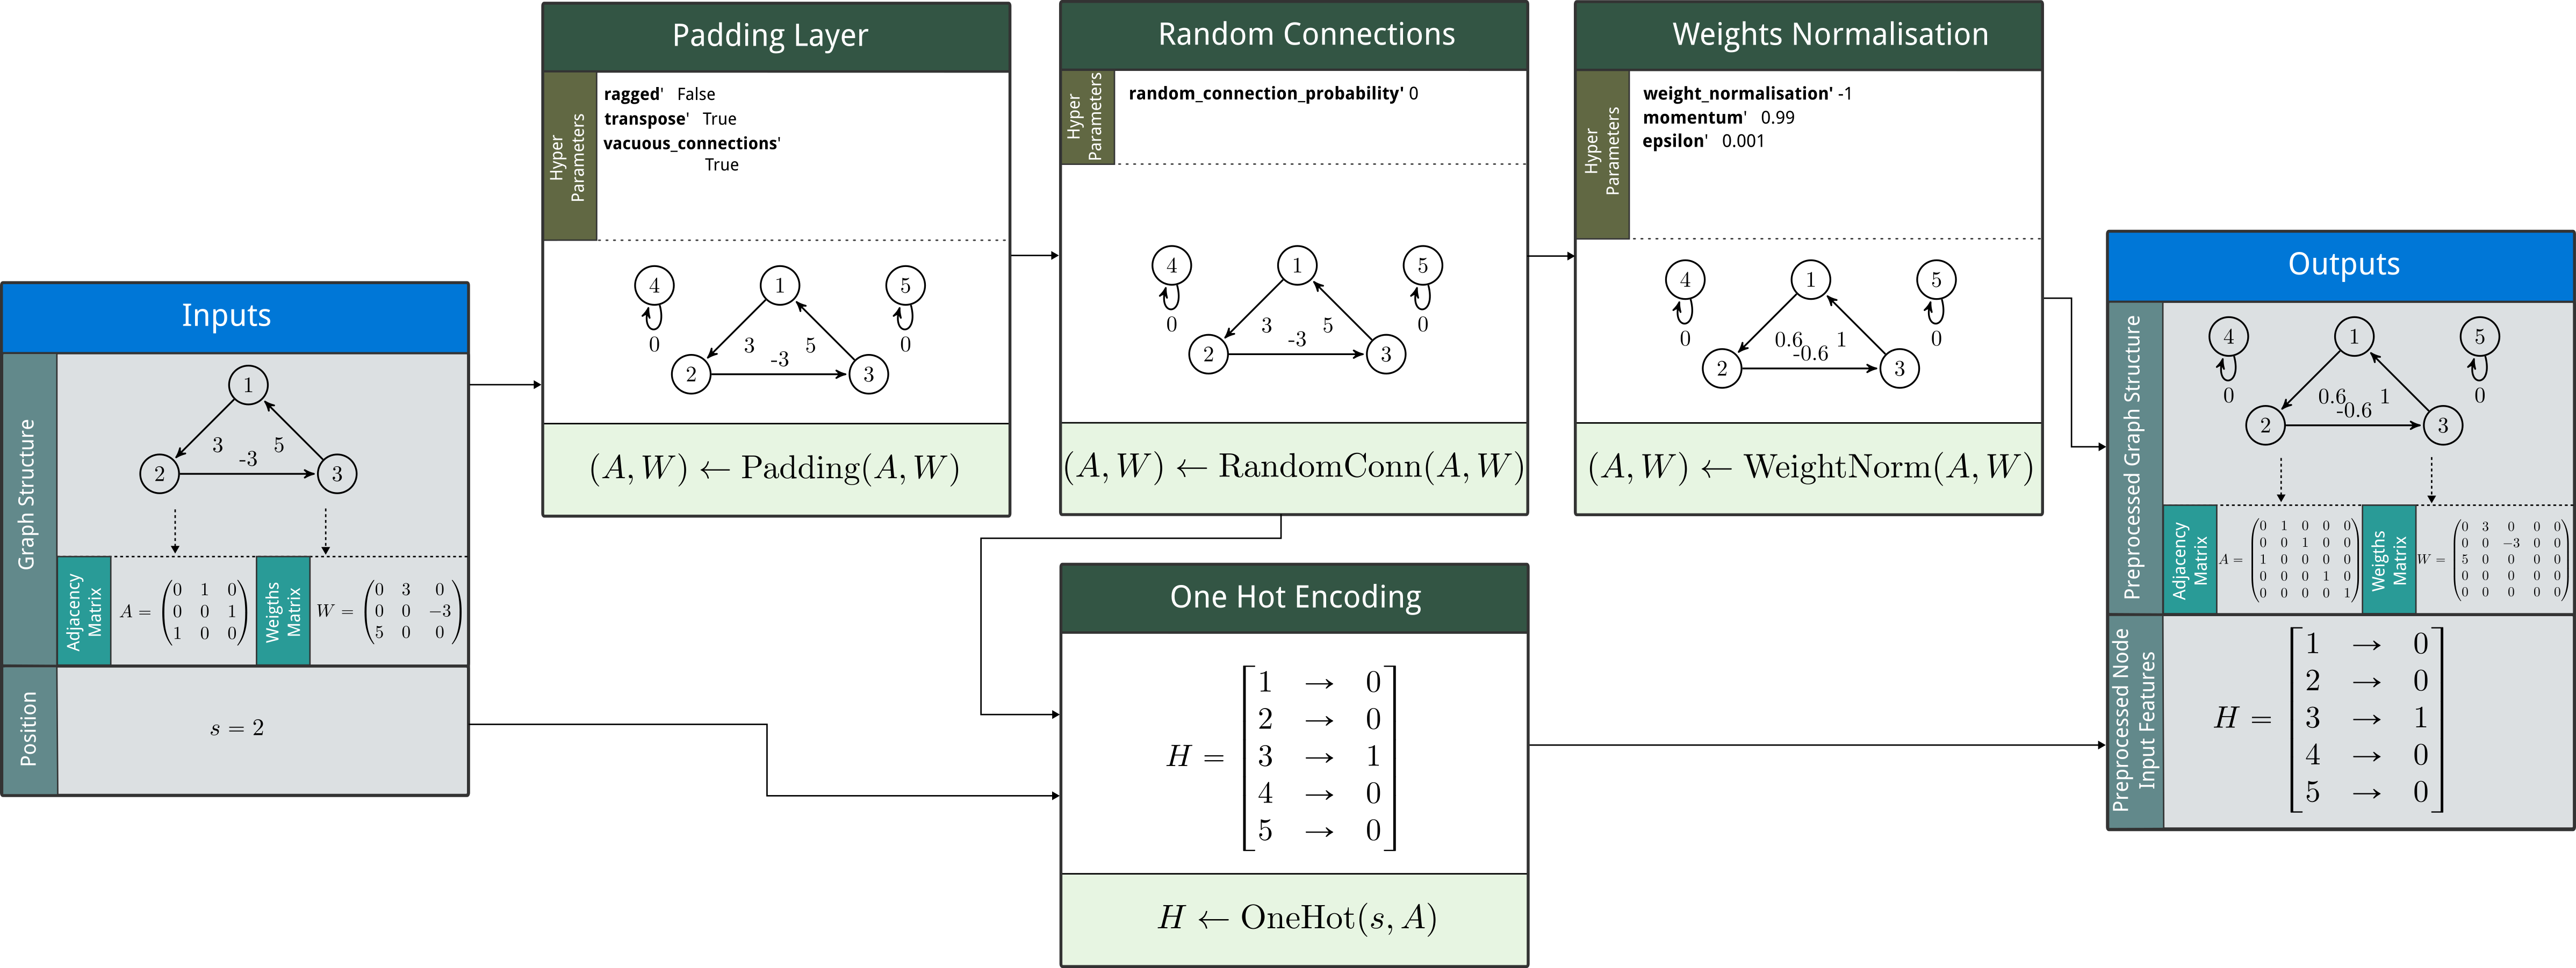
\includegraphics[width=1.2\textwidth]{Figures/PreprocessingBlock.png}}
	\caption{Preprocessing Block}
	\label{fig:PreprocessingBlock}
\end{figure}
\newpage

\subsection{Weighted Graph Convolutional Network}
The weighted graph convolutional network \textbf{WGCN}, as its name suggests, is a convolutional operator acting on graphs, with many desirable properties such as ``Permutation Equivariance" and ``Stability under Padding".
\newline It is based on the graph convolutional network as described on the following figure
\begin{figure}[H]
	\noindent
	
	\makebox[\textwidth]{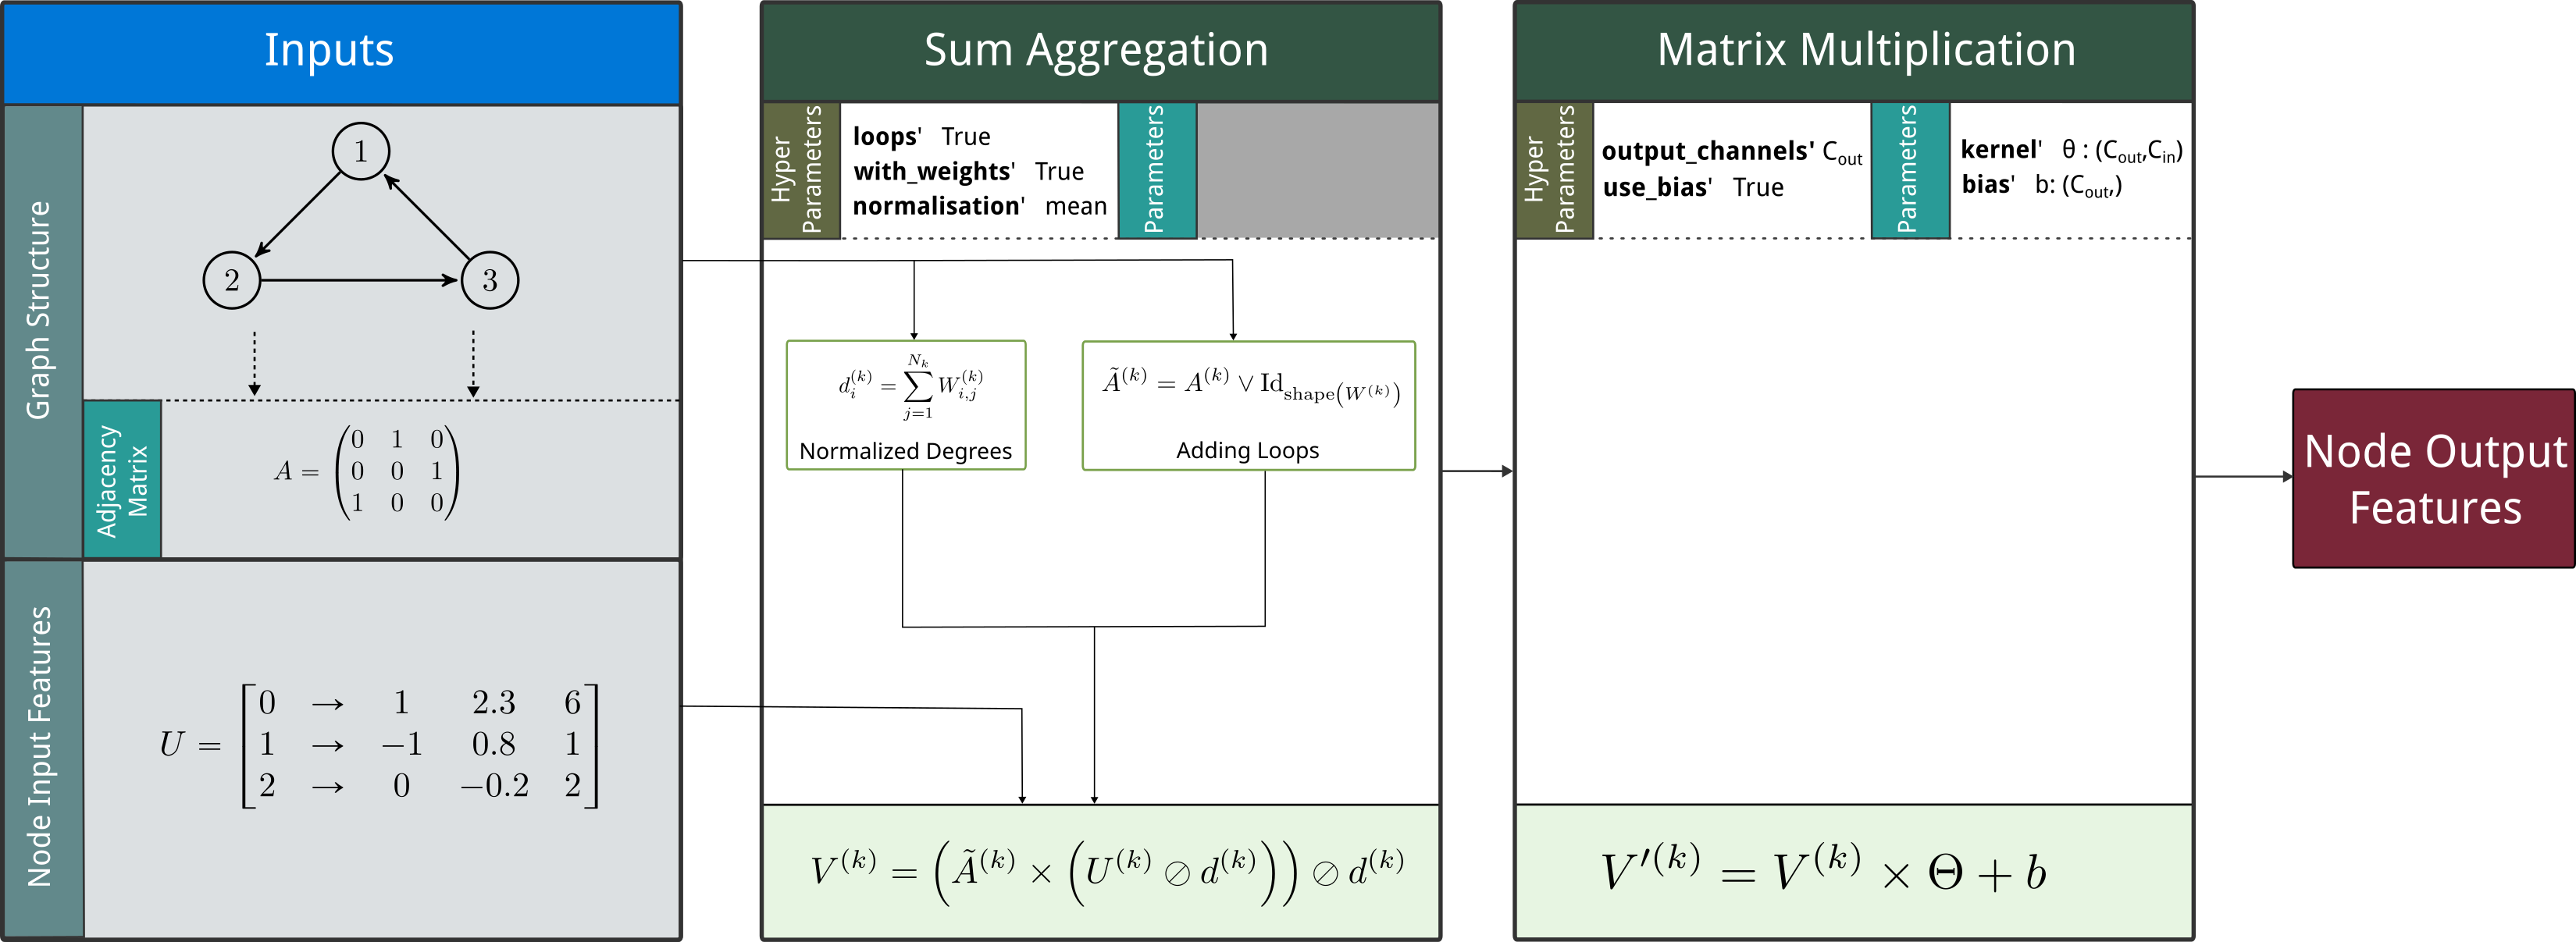
\includegraphics[width=1.2\textwidth]{Figures/GCN.png}}
	\caption{Graph Convolutional Network}
	\label{fig:GCN}
\end{figure}
\FloatBarrier
Here $\oslash$ denotes the point-wise division operator.
\newline 
The problem with \textbf{GCN} is that they ignore the weights information. For Mean Payoff Games, such information is crucial to determine the winner and the strategies.
\newline For that, we introduced \textbf{WGCN} to capitalize on the weights information. The figure below shows how it is implemented.

\begin{figure}[H]
	\noindent
	
	\makebox[\textwidth]{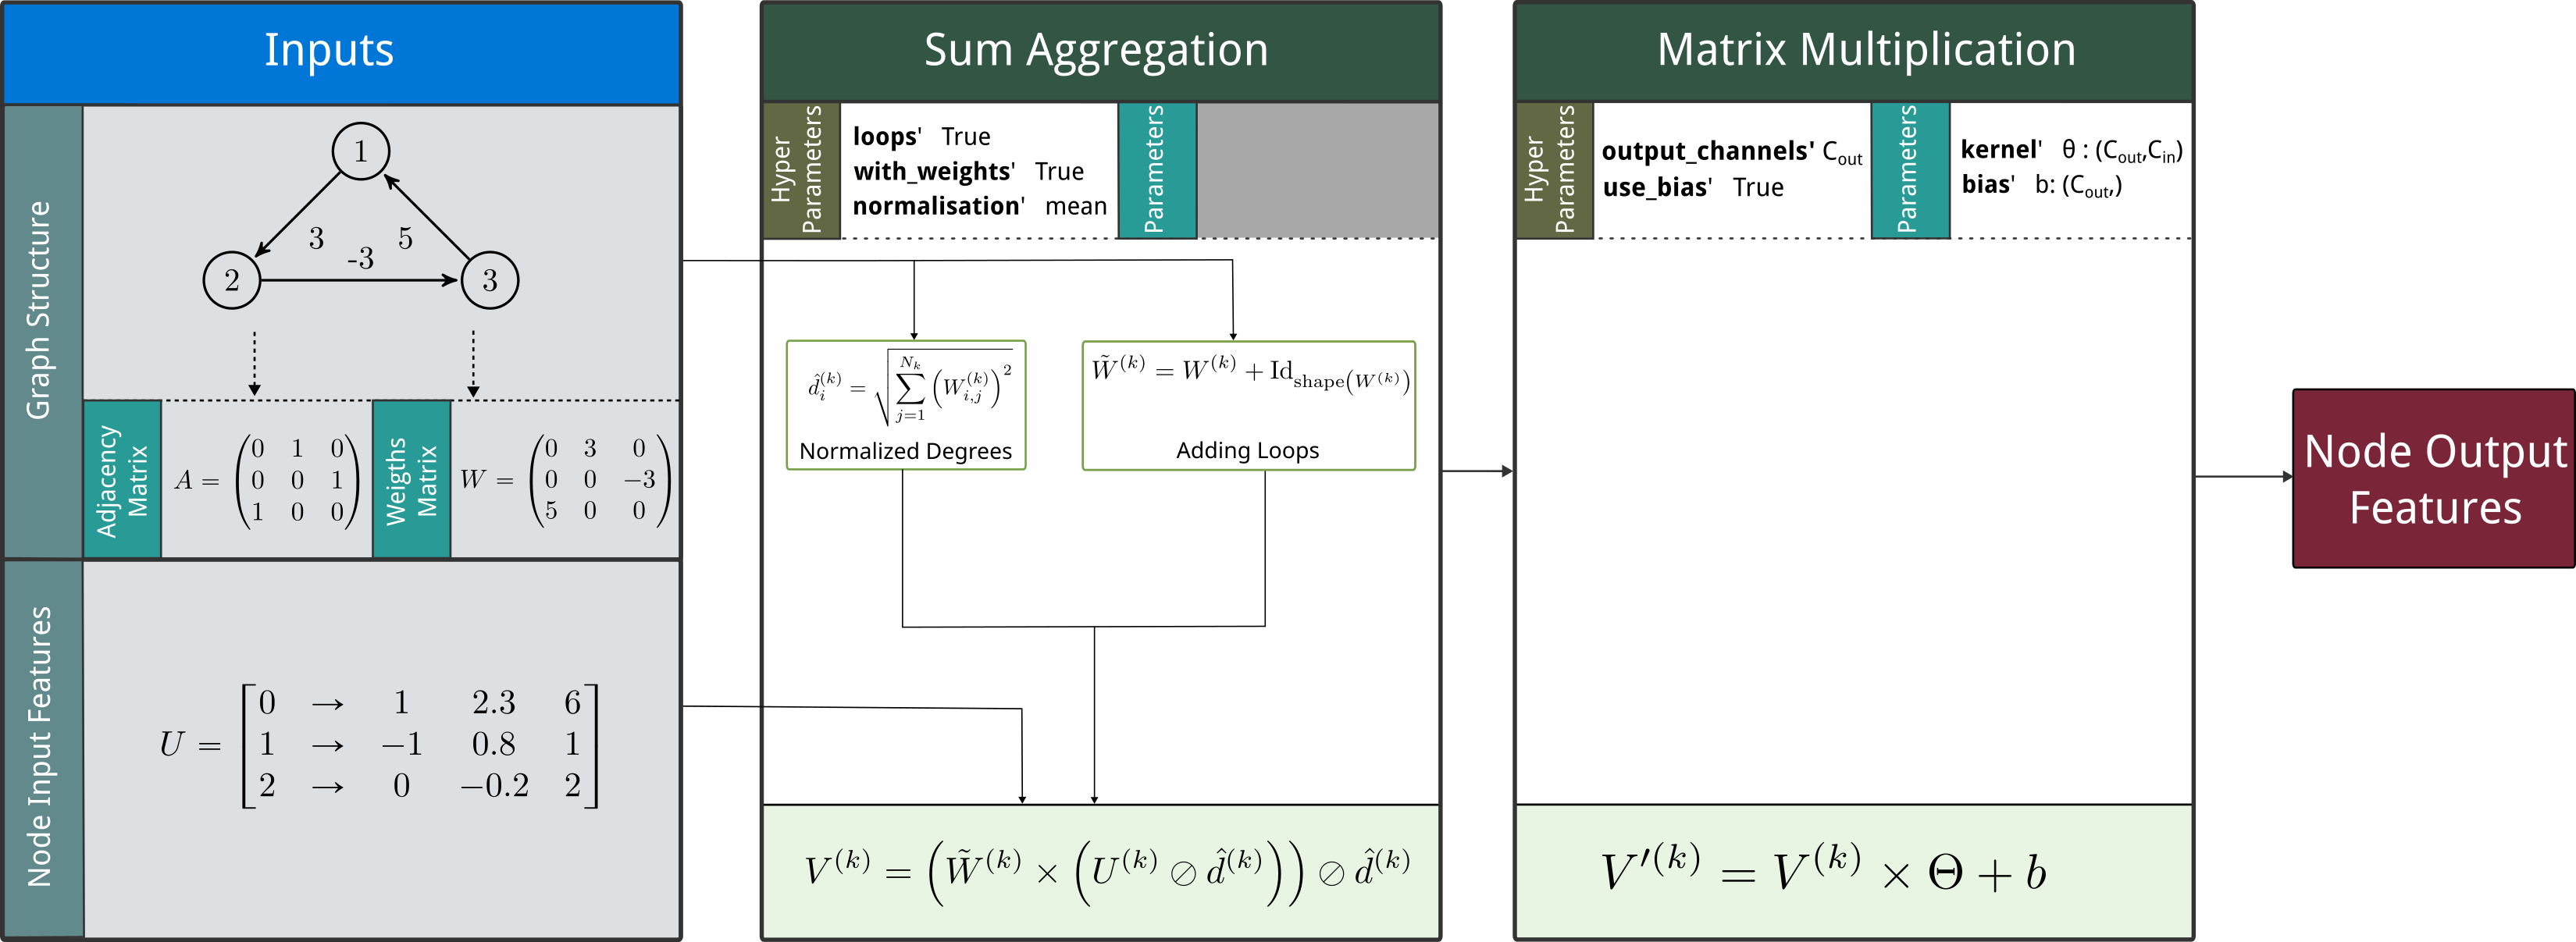
\includegraphics[width=1.2\textwidth]{Figures/WGCN.png}}
	\caption{Weighted Graph Convolutional Network \label{fig:WGCN}}
\end{figure}
\FloatBarrier
The \textbf{WGCN} operator exhibits the desired properties described on \ref{section:ModelDesign:Properties}, except property  \ref{section:ModelDesign:Properties:Invariance}, the latter is already verified as a result of the preprocessing layer.
\newline We were not able to find a reference to \textbf{WGCN} in the literature. The closest thing we have found that a PyTorch based GNN library named \textbf{Geometric} has an implementation for \textbf{GCN} supporting weighted graphs. Interestingly, we only differ to them by the normalization of the degrees.
\newline As we are using \textit{TensorFlow}, we cannot use their approach, so we had to implement \textbf{WGCN} from scratch.

\subsection{Convolutional Block}
Each intermediate block is composed of a graph convolution, and then a batch normalisation operator, as described by the figure below:
\begin{figure}[H]
	\noindent
	
	\makebox[\textwidth]{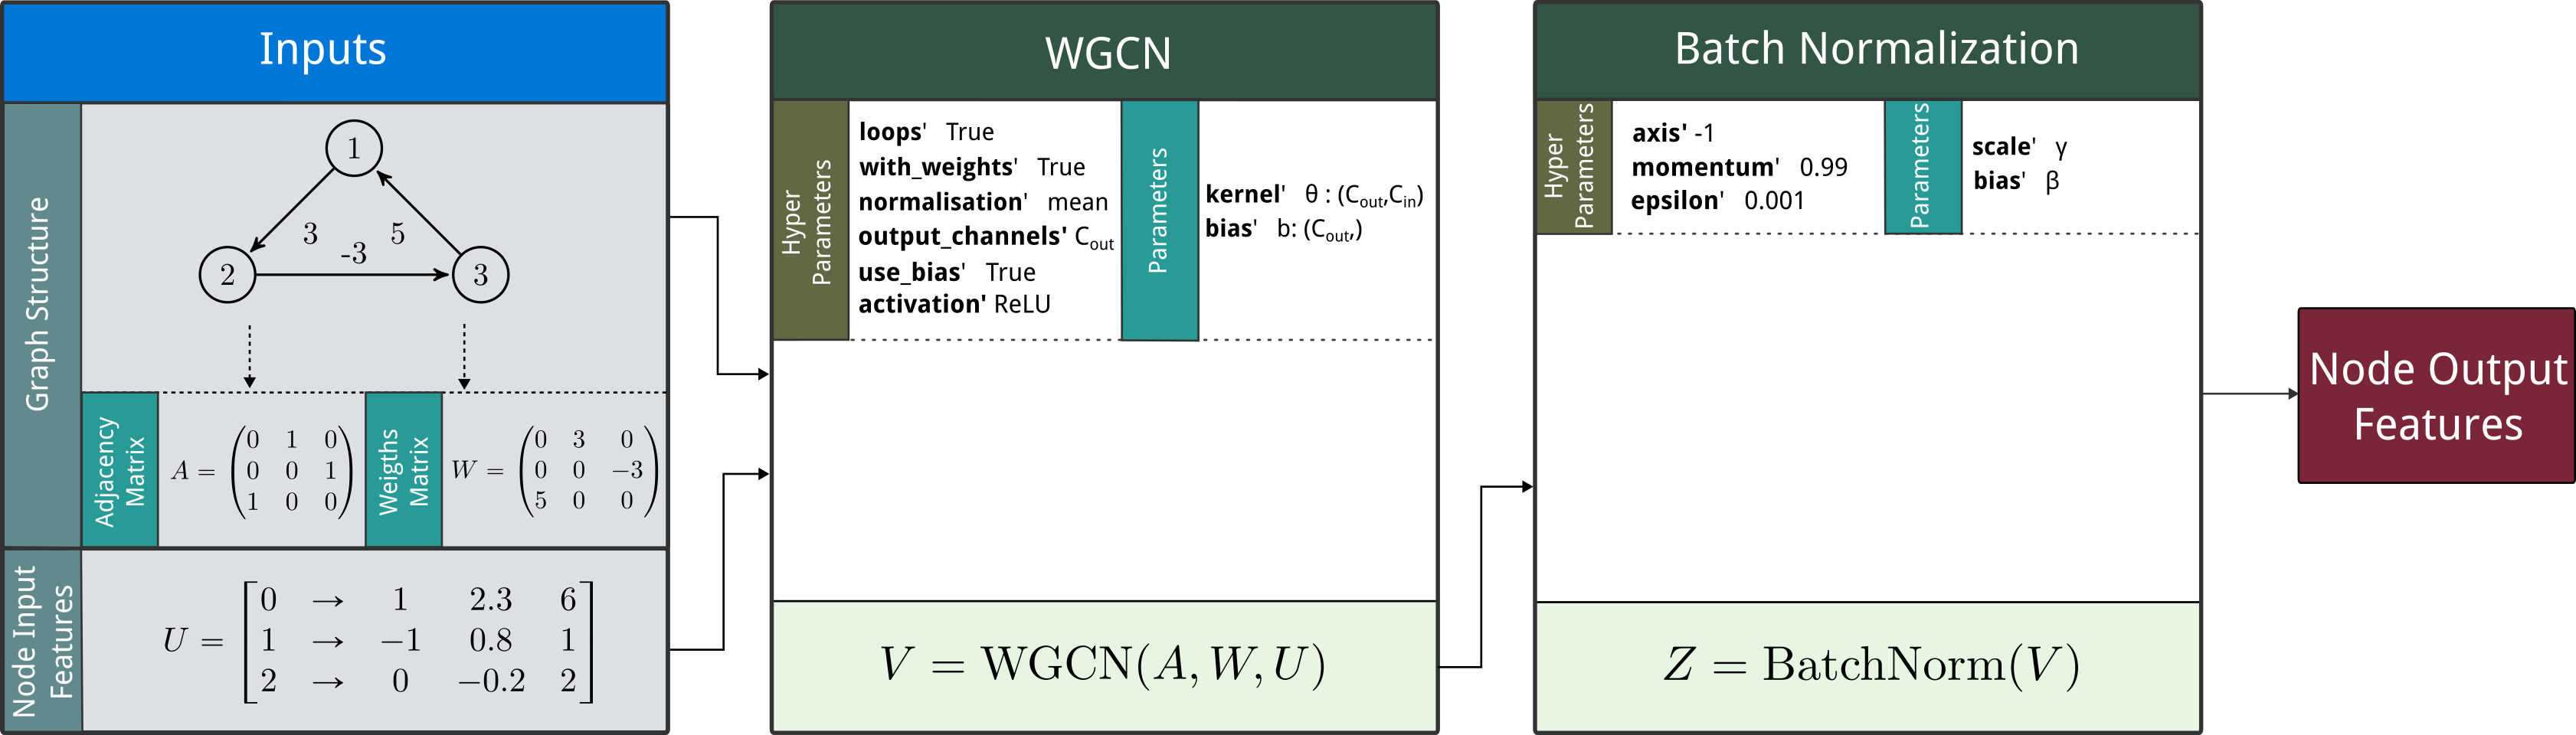
\includegraphics[width=1.2\textwidth]{Figures/ConvolutionalBlock.png}}
	\caption{Graph Convolutional Block}
	\label{fig:ConvolutionalBlock}
\end{figure}
\FloatBarrier
This block was inspired from convolutional blocks used in computer vision models.
\subsection{Prediction Block}
\begin{figure}[H]
	\noindent
	
	\makebox[\textwidth]{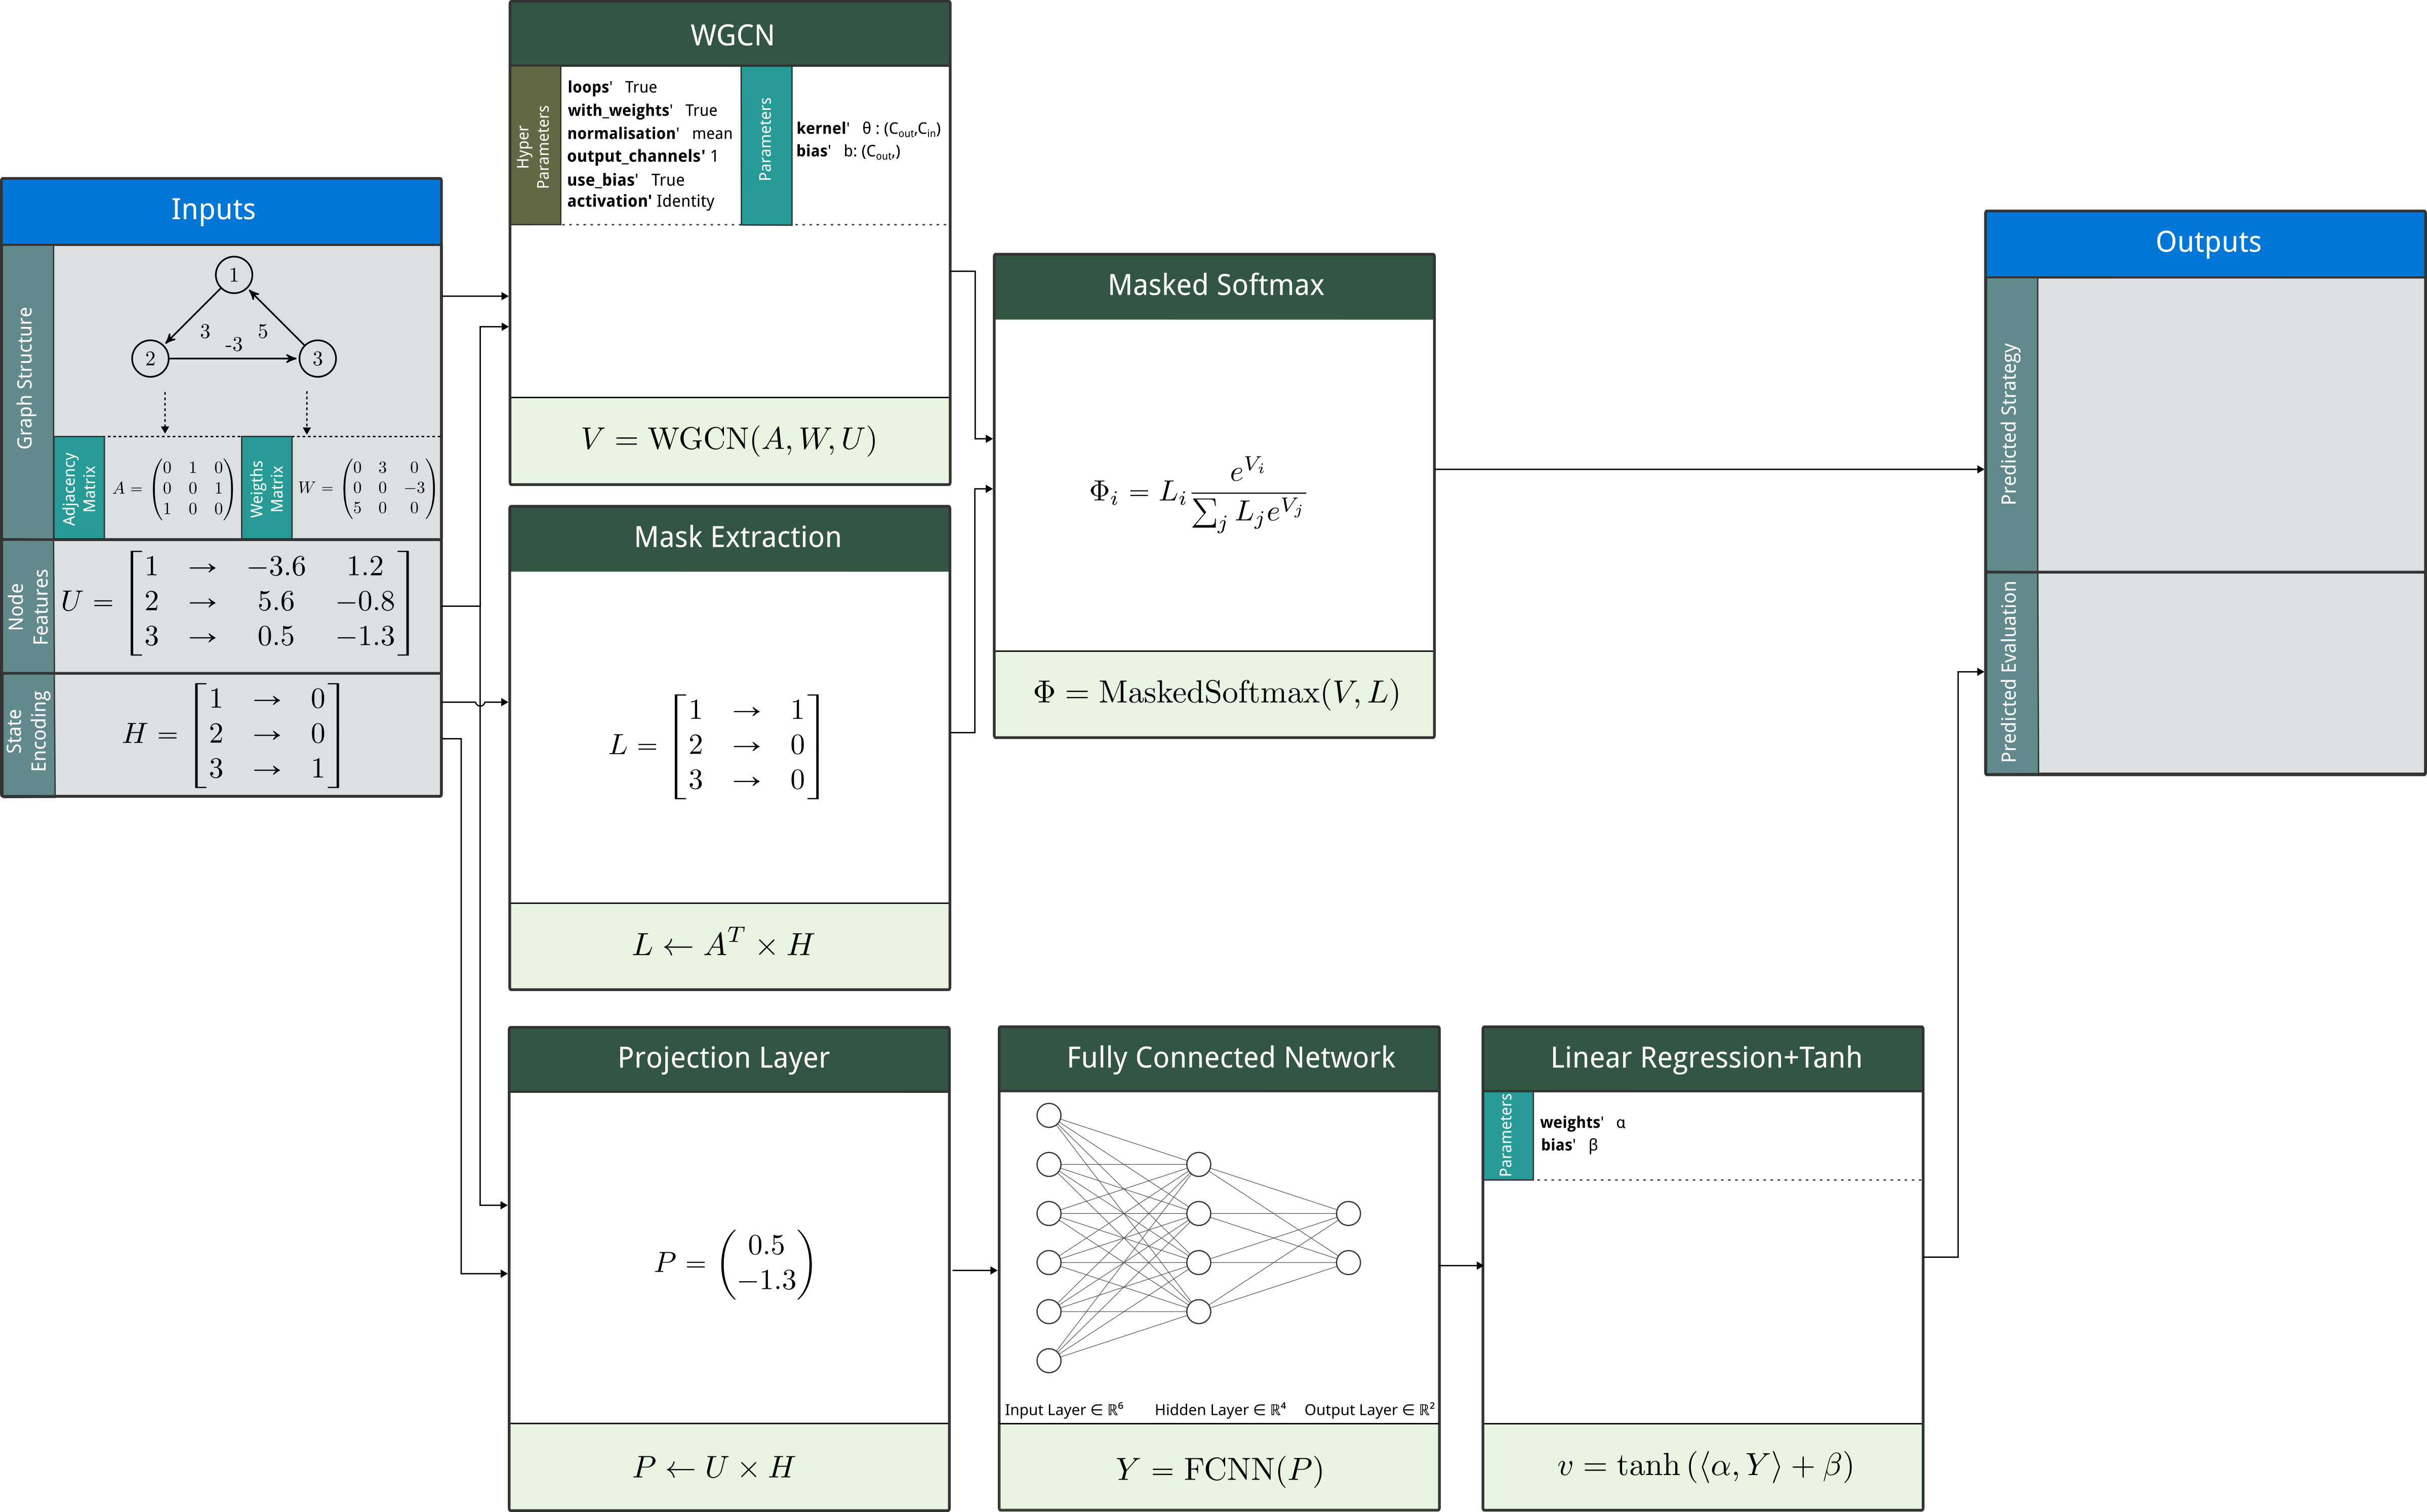
\includegraphics[width=1.2\textwidth]{Figures/PredictionBlock.png}}
	\caption{Graph Convolutional Block}
	\label{fig:PredictionBlock}
\end{figure}
\FloatBarrier
\subsection{Model Architecture}
Putting all building block together, we designed a model that takes arbitrary graphs, encode them, predicts the strategy and the evaluation of the position.
\newline We were very careful in the design so that we can verify all the desired properties described in section \ref{section:ModelDesign:Properties}.
\newline The figure below shows the whole architecture:

\begin{landscape}

	\begin{figure}[H]
	\centering
		
		{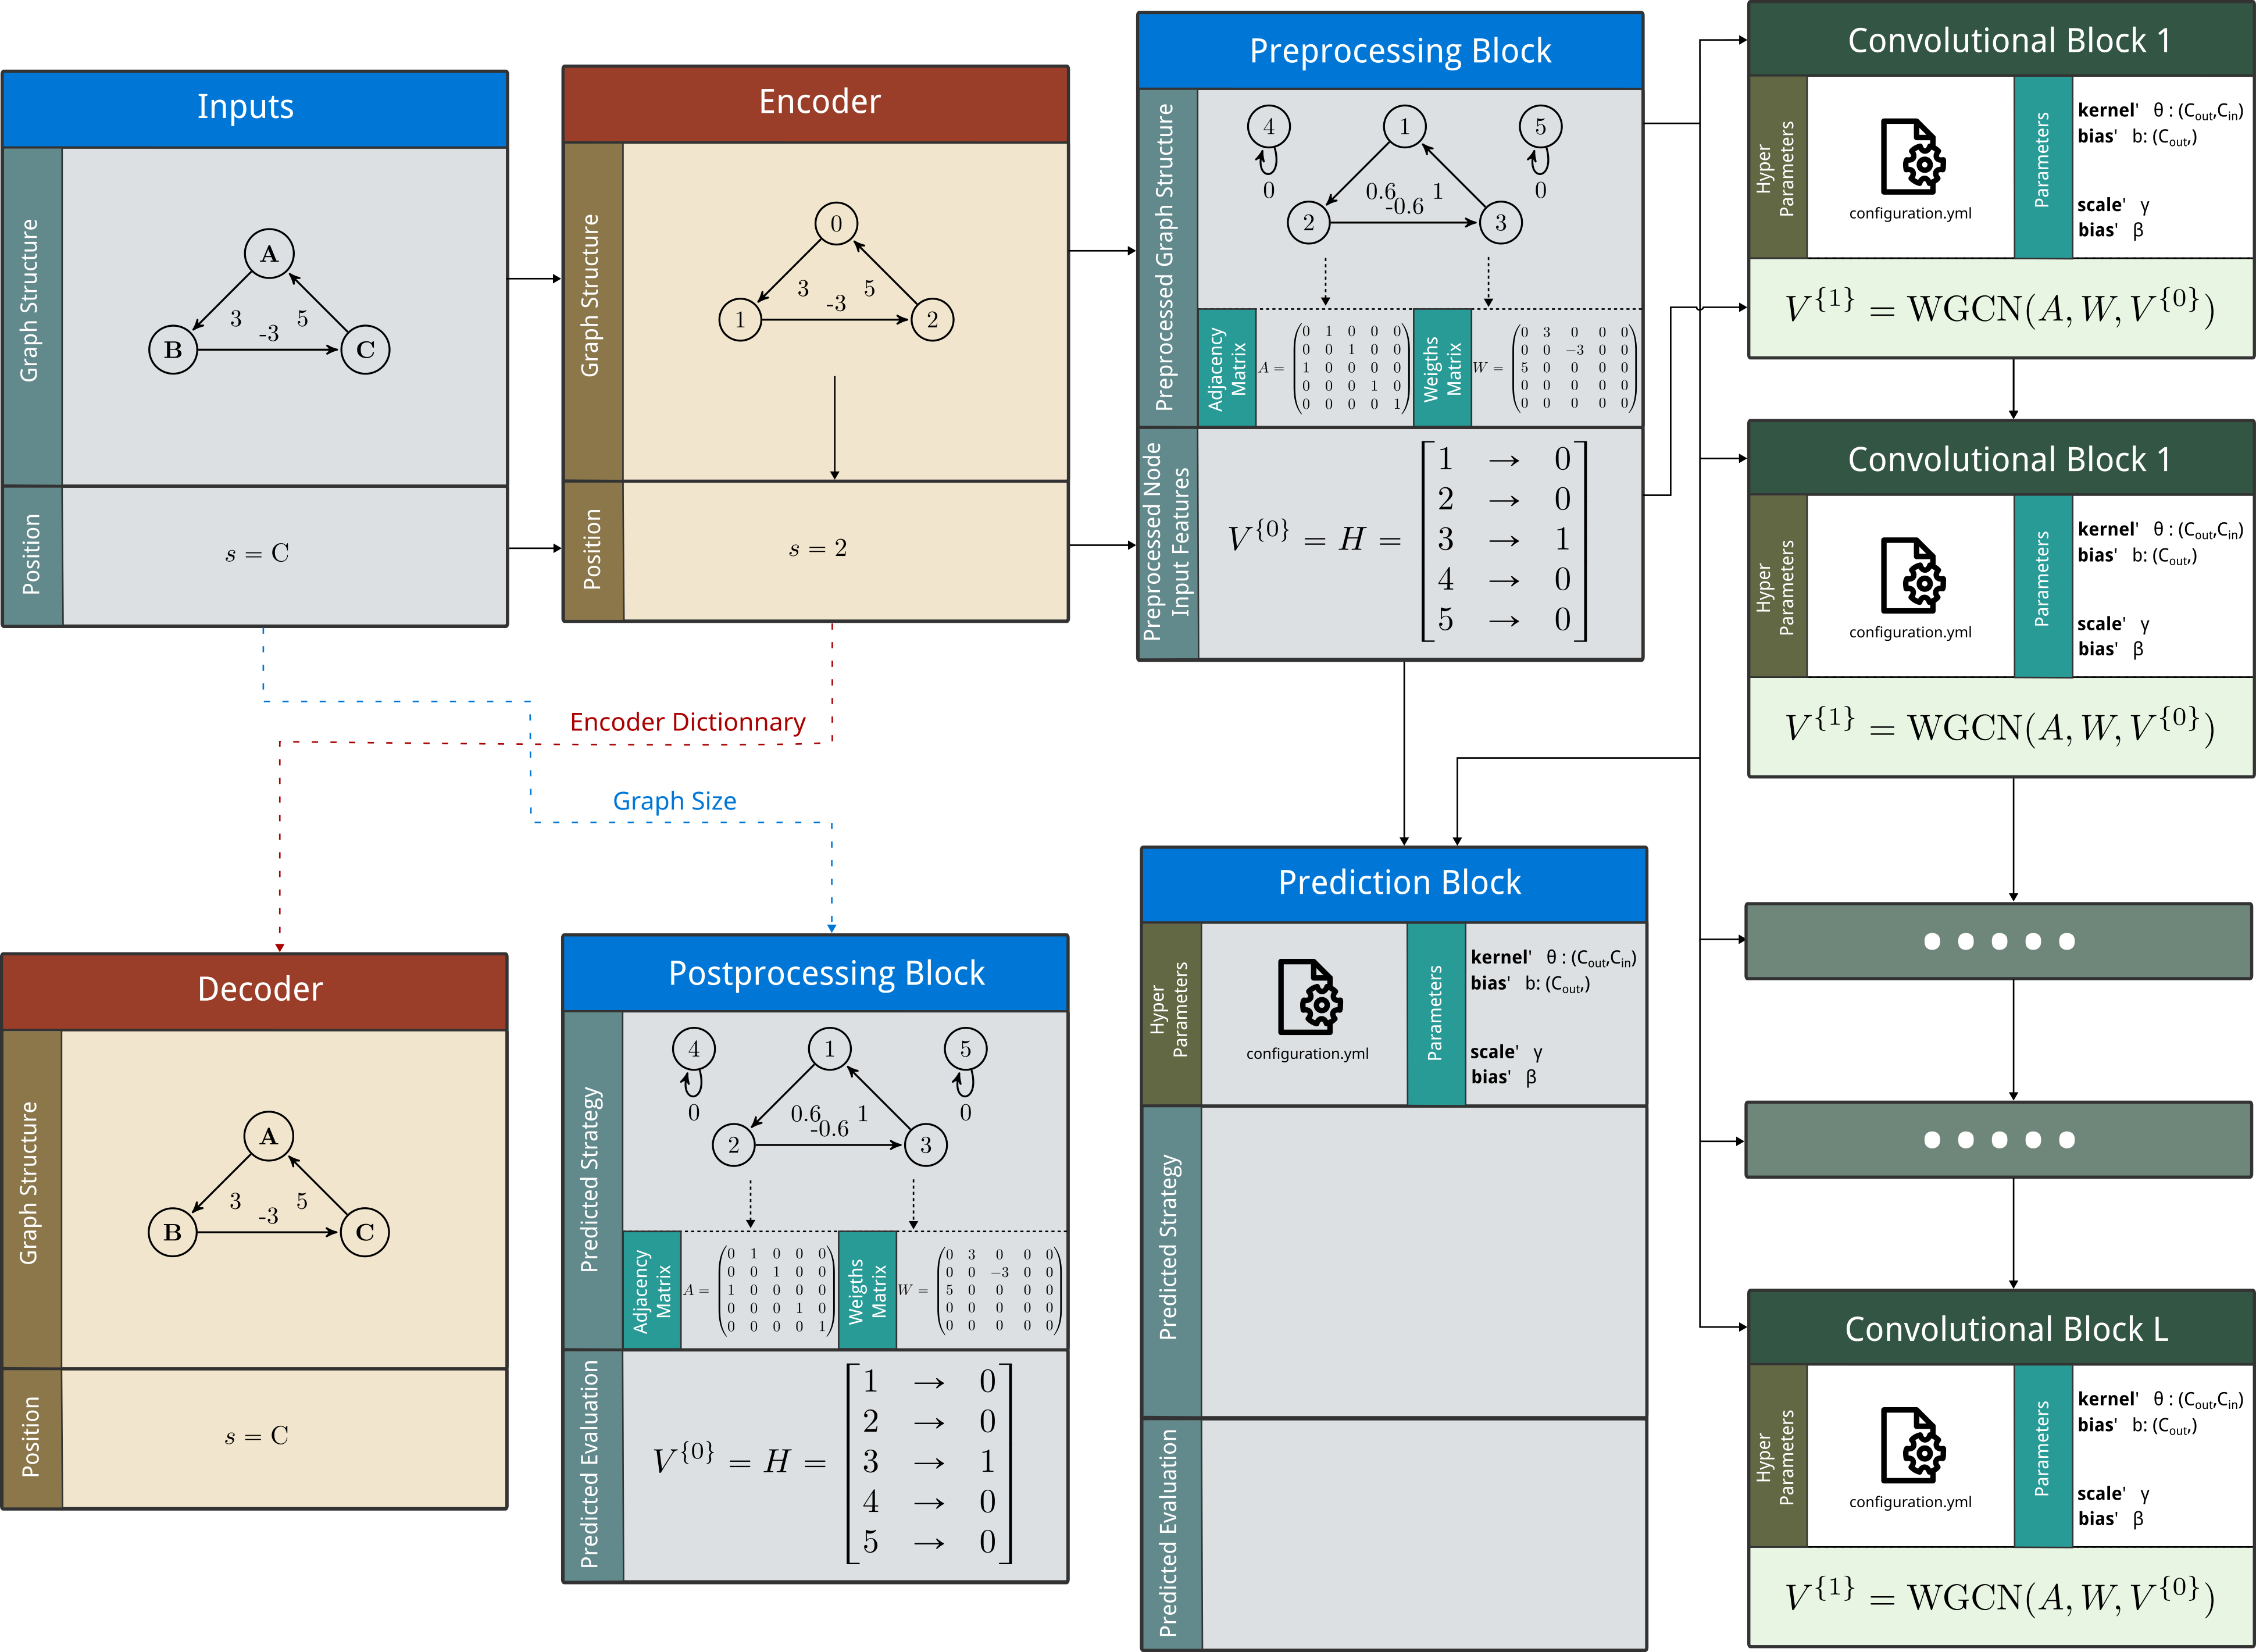
\includegraphics[height=0.93\textheight]{Figures/Architecture.png}}
		\caption{Model Architecture}
		\label{fig:ModelArchitecture}
	\end{figure}
	
\end{landscape}

\section{Optimization}
Once we built the model architecture, we have to define the optimization problem to refine the learnable parameters.

Also, there is a wide range of optimizers that we can use. The next two sections will respectfully define the loss function and the optimizer.
\subsection{Loss function}
\begin{itemize}
	\item Let $\boldsymbol{G}$ be a batch of \acrshortpl{mpg}.
	\item Let $\boldsymbol{v}$ be a batch of evaluations of $\boldsymbol{G}$ 
	\item Let $\boldsymbol{\Pi}$ be a batch of strategies of $\boldsymbol{G}$
	\item Let $\mathcal{M}_{\Theta}$ be the model with $\Theta$ the learnable parameters.
	\item Let $\boldsymbol{v}_{\Theta}$ be the predicted evaluation per model $\mathcal{M}_{\Theta}$
	\item Let $\boldsymbol{\Pi}_{\Theta}$ be the predicted strategy per model $\mathcal{M}_{\Theta}$ 
	\item Let $\mathcal{H}$ be the categorical cross entroy operator defined as follow:
	\begin{equation*}
		\mathcal{H}(p,q) = \sum_{i}p_i \log q_i 
	\end{equation*}
\end{itemize}
We defined the loss function similar to Alpha Zero's approach \cite{AlphaZero}:
\begin{equation}
	\label{eqn:LossFunction}
	\mathcal{L}(\mathcal{M}_{\Theta},\boldsymbol{G},\boldsymbol{v},\boldsymbol{\Pi}) = \mathcal{H}(\boldsymbol{\Pi},\boldsymbol{\Pi}_\Theta(\boldsymbol{G})) + \lVert \boldsymbol{v}_{\Theta}(\boldsymbol{G})- \boldsymbol{v} \rVert_2^2 +  C \lVert \Theta \rVert_2^2
\end{equation}
This is the sum of three terms:
\begin{itemize}
	\item $\displaystyle \mathcal{H}(\boldsymbol{\Pi},\boldsymbol{\Pi}_\Theta(\boldsymbol{G})):$ This term encodes the error between the predicted strategy $\boldsymbol{\Pi}_\Theta(\boldsymbol{G})$ and the actual strategy $\boldsymbol{\Pi}$.
	\item $\displaystyle \lVert \boldsymbol{v}_{\Theta}(\boldsymbol{G})- \boldsymbol{v} \rVert_2^2:$ This term encodes the euclidean distance between the predicted evaluation $\boldsymbol{v}_{\Theta}(\boldsymbol{G})$ and the actual evaluation $\boldsymbol{v}$.
	\item $\displaystyle C \lVert \Theta \rVert_2^2$ This term adds $L_2$ regularization to the model, with $C$ serving as the strength of the regularization.
\end{itemize}
Also, each error term in the loss function is applied to each game individually. In fact, equation \eqref{eqn:LossFunction} is in a compact representation that reduces\footnote{Up to some normalization factor, this is an implementation detail.} to the mean of individual errors in the batch.
\subsection{Optimizer}
We used the Adam optimizer \cite{AdamOptimizer} to minimize the objective function $\mathcal{L}$ with respect to $\Theta$

\subsection{Hyper-parameters}
Our choice of optimizer and loss function induced more hyper-parameters. We will list them in the following table:


\section{Configuration}
we externalized our configuration so that we can change hyperparameters and other non-learnable parameters at will, without modifying the source code. This was beneficial as it seperated between the model implementation phase and the model fine-tuning phase.
\subsection{Model configuration}
We setup a configuration YAML configuration file containing the entries for tweaking the model.
\begin{figure}[H]
	\centering
	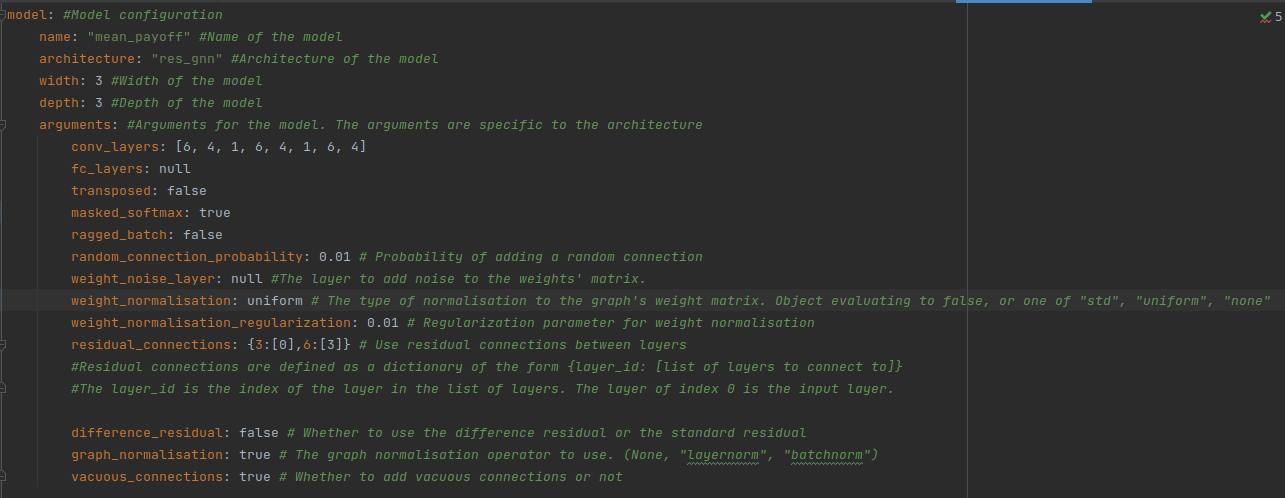
\includegraphics[width=0.95\textwidth]{Figures/ModelConfiguration.png}
	\caption{Model section of the configuration file}
	\small{Note: while a recent version of the configuration file, we may tweak it further for fine-tuning purposes.}
\end{figure}
\FloatBarrier
\subsection{Training configuration}
The configuration file also has a section for training hyper-parameters. We will show it in the next figure:
\begin{figure}[H]
	\centering
	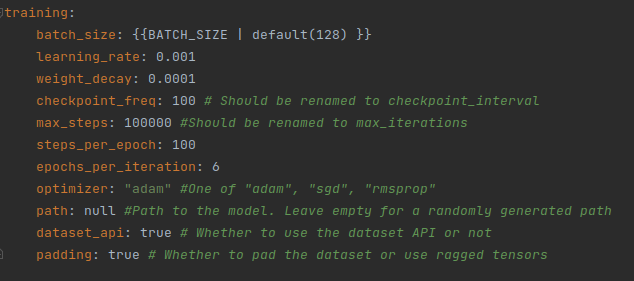
\includegraphics[width=0.75\textwidth]{Figures/TrainingConfiguration.png}
	\caption{Training section of the configuration file}
	\small{Note: while a recent version of the configuration file, we may tweak it further for fine-tuning purposes.}
\end{figure}
\chapter{Pipeline Architecture}

\section{Pipeline}
\section{Services}
\section{Configuration}

\chapter{Analyse}

For $x\in \mathcal{X},Y\subseteq\mathcal{X}^m,c\in I$, let $\text{MA}(x,Y,c)$ be defined as follow:
$$
\text{MA}(x,Y,c)\iff x\le \max Y+c
$$
\gls{ny} Hi
\chapter*{Conclusion \& Perspectives}
\addcontentsline{toc}{chapter}{Conclusion \& Perspectives}

In this internship, we  \\
\\
Dans le premier chapitre, nous avons présenté \textbf{dB Sense} et ses activités. \\
\\
Dans le deuxième chapitre, nous avons présenté le problème de la grande complexité, introduit le concept des BNNs et proposé \textbf{binaryflow} comme notre solution pour les BNNs\\
\\
Dans le troisième chapiter, nous avons formalisé les BNNs, et nous avons décris leurs optimisations possible, et les problèmes rencontrés dans leur implémentation.\\
\\
Dans le quatrième chapitre, nous avons présenté des modèles BNNs, chacun en dérivant ses formules\\
\\
Dans le cinquième chapitre, nous avons donné notre implémentation de \textbf{binaryflow} en jusitifiant les paradigmes utilisés\\
\\
Dans le sixième chapitre, nous avons analysé 3 jeux de données en implémentant des modèles BNNs pour chacune de ces 3 jeux de données, et en comparant les performances de prédicition et la complexité temps et mémoire des modèles entraînés.\\
\\
Notre travail n'est qu'une petite introduction des BNNs. En effet, la liste des BNNs proposés dans la littérature est très vaste, et il existe plusieurs autres approches pour faciliter l'entraînement et l'interférence des BNNs que nous n'avons pas considéré vu les contraintes de stage, y parmi:
\begin{enumerate}
	\item Les méthodes d'optimisations discrètes
	\item Les optimiseurs dédiés au BNNs
	\item Les binarisations entraînables
	\item Les méthodes ensemblistes pour régulaliser les BNNs
\end{enumerate} 
De plus, nous avons réussi à vérifier l'optimisation de la multiplication matricielle (L'éxecution est parfois 30 fois plus rapide), mais nous n'avons pas pu intégrer cette optimisation aux modèles tensorflow. Et malgré que larq supporte lui même un déploiement optimisé, nous n'avons pas aussi pu l'exploiter puisque ce déploiement ne supporte que les processeurs ARMv8, et nous utilisons une machine avec un processeur d'architecture x86-64.\\
\\
Finalement, nous avons fait une petite intégration du code carbone comme une mésure de coût d'entraînement. Une fois le problème de déploiement est résoulu, nous recommenderions l'utilisation de ce même métrique pour estimer le coût d'interférence qui va justifier l'utilisation des BNNs.   
\appendix
\chapter{On Constraint Satistfaction Problems}
\label{appendix:CSP}
In the previous chapters, we described how the system works, without formalising the CSP approach.\newline
On this chapter, we will describe the CSP systems that we have used, with an equivalence proof between them.

\section{Constraint Satisfaction Problem}
\subsection{Definition}
A constraint satisfaction problem
\subsection{Assignment}
An assignment of a $\CSP(\mathcal{X},D,\Gamma)$ is a function $X:\mathcal{X}\rightarrow D$ such that, by replacing each $x\in\mathcal{X},$ by $X(x),$ all the constraints will evaluate to $\True$
\subsection{Polymorphism}
A function $F:\mathscr{F}(\mathcal{X},D)^k\rightarrow \mathscr{F}(\mathcal{X},D)$ is said to be a polymorphism if:
$$
\forall X_1,\dots,X_k \ \text{assignments of}\ \CSP(\mathcal{X},D,\Gamma),\quad F(X_1,\dots,X_k) \ \text{is also an assignment of}\ \CSP(\mathcal{X},D,\Gamma)
$$
Now, in the next section, we will define an important class of CSPs that is used to solve Mean Payoff Games, with the polymorphisms required for the solution algorithm's correctness

\section{Ternary Max Atom Systems}
\subsection{Definition}
\begin{itemize}
	\item Let $\mathcal{X}$ be a finite set of variables
	\item Let $D=I\cup \{-\infty\},$ with $I\subseteq \mathbb{R}$.
	\item  For $x,y,z\in \mathcal{X},c\in I$, let $\text{MA}_3(x,y,z,c)$ be defined as follow:
	$$
	\text{MA}_3(x,y,z,c)\iff x\le \max(y,z)+c
	$$
\end{itemize}
A ternary max atom system is $\CSP(D,\Gamma)$ where:
\begin{align*}
	\Gamma&=\left\{\text{MA}_3(x,y,z,c),\quad (x,y,z,c)\in \mathscr{R}\right\}\\
	\mathscr{R}&\subseteq \mathcal{X}^3\times I\\
	\mathscr{R}& \space \text{is finite}
\end{align*}
\subsection{Example}
An example of a ternary max atom system is the following $\CSP(D,\Gamma)$ with $D=\mathbb{Z}$ and $\Gamma$ represented as follow:
\begin{align*}
	x &\le \max(y,z)-1 \\
	y &\le \max(z,x)-1 \\
	z & \le \max(x,y)-1
\end{align*}


\section{Max Atom Systems}
\subsection{Definition}
\begin{itemize}
	\item Let $\mathcal{X}$ be a finite set of variables
	\item Let $D=I\cup \{-\infty\},$ with $I\subseteq \mathbb{R}$   
	\item For $x\in \mathcal{X},Y\subseteq\mathcal{X}^m,c\in I$, let $\text{MA}(x,Y,c)$ be defined as follow:
	$$
	\text{MA}(x,Y,c)\iff x\le \max Y+c
	$$
\end{itemize}

A max atom system is $\CSP(D,\Gamma)$ where:

\begin{align*}
	\Gamma&=\left\{\text{MA}(x,Y,c),\quad (x,Y,c)\in \mathscr{R}\right\}\\
	\mathscr{R}&\subseteq \mathcal{X}\times \left(\mathscr{P}(\mathcal{X}) \setminus \{\varnothing\}\right)\times I \\
	\mathscr{R}&\space \text{is finite}
\end{align*}

\subsection{$\text{MA} \le \text{MA}_3$}
\begin{itemize}
	\item Let $S=\CSP(\mathcal{X},D,\Gamma)$ a max atom system.
	\item Let $R\in \Gamma$
	\item Let $x\in \mathcal{X},Y\in\mathscr{P}(\mathcal{X}),c\in I$ such that $R=\text{MA}(x,Y,c)$ such that $\lvert Y \rvert >2$
\end{itemize}

\subsubsection{Recursive Reduction}
We will reduce the arity of $R$ as follow:
\begin{itemize}
	\item Let $y,z\in Y$ such that $y\ne z$
	\item We introduce a variable $w\notin \mathcal{X}$
	\item Let $\mathcal{X}'=\mathcal{X}\cup\{w\}$
	\item Let $Y'=(Y\cup \{w\})\setminus\{y,z\}$
	\item Let $R'=\text{MA}(x,Y',c)$
	\item Let $R_w=\text{MA}(w,\{y,z\},0)$
	\item Let $\Gamma'=(\Gamma\cup\{R',R_w\})\setminus \{R\}$
	\item Let $S'=\CSP(\mathcal{X}',D,\Gamma)$
\end{itemize}


We will prove that $S'$ is equivalent to $S.$

\paragraph{Implication}
Let $X:\mathcal{X}'\rightarrow D$ an assignment of $S'.$ It is trivial that by removing $X(w)$, $X_{\mid \mathcal{X}}$ is an assignment of $S$ 

\paragraph{Equivalence}
\begin{itemize}
	\item Let $X:\mathcal{X}'\rightarrow D$ such that $X_{\mid \mathcal{X}}$ is an assignment of $S.$
	\item We will set $X(w)=\max(X(y),X(z))$
\end{itemize}
Then, $X$ is an assignment of $S'$

\subsubsection{Induction}
Since the number of variables is finite, the arity of each constraint is finite. Also, as the the number of constraints is finite, Applying such reduction iteratively will eventually give a system $S^*$ equivalent to $S$ with:
\begin{itemize}
	\item $\mathcal{X}^*$ the set of variables with $\mathcal{X}\subseteq \mathcal{X}^*$ 
	\item $\Gamma^*$ is the set of constraints:
	\item Each constraint is of the form $\text{MA}(x,Y,c)$ with $x\in \mathcal{X}^*,Y\subseteq \mathcal{X}^*,c\in I$ with $\lvert Y\rvert \le 2$   
\end{itemize}
Now such system can be transformed to a ternary system $S_3$ as follow:
\begin{itemize}
	\item The set of variables is $\mathcal{X}^*$
	\item The domain is $D$
	\item For every relation $R=\text{MA}(x,Y,c)$ we map it to the relation $R_3=\text{MA}(x,y,z,c)$ as follow:
	\begin{itemize}
		\item If $\lvert Y \rvert=2$, then $y,z$ are the elements of $Y.$
		\item Otherwise, $\lvert Y \rvert=1,$ and $y=z$ are the same element of the singleton\footnote{A set with only one element} $Y.$
	\end{itemize}
	
\end{itemize}


It is trivial that $S^*$ is equivalent to $S_3.$
With that, $S$ is equivalent to $S_3.$


\begin{algorithm}
	\caption{Converting a Max Atom System to Ternary Max Atom System}\label{alg:MaxAtomToTernaryMaxAtom}
	\begin{algorithmic}
		\Require $S$ an $N$-ary Max Atom system
		\Ensure $S'$ a ternary Max Atom system  
		\State $S'\leftarrow \varnothing$
		\State $H\leftarrow\varnothing$ \Comment{$H$ is a symmetric map between variable,variable to variables}
		\State $V\leftarrow \text{Variables}(S)$  \Comment{$V$ is a set containing all variables}
		\For {$\mathcal{C}\in S$}
		\Comment{Iterate over constraints}
		\State $c$ is the constant in the right hand side of $\mathcal{C}$
		\State $Y$ is the variables in the right hand side of $\mathcal{C}$
		\State $x$ is the variable in the left hand side of $\mathcal{C}$
			\While{$\lvert Y \rvert > 2$}
				\State $y\leftarrow \pop(Y)$
				\State $z\leftarrow \pop(Y)$
				\If {$(y,z) \notin \domain  H$}
					\State $w\leftarrow \text{newVariable}(V)$\Comment{Generate a new formal variable not included in $V$}
					\State $V\leftarrow V\cup\{w\}$
					\State $H(y,z)\leftarrow w$
					\State $H(z,y)\leftarrow w$
				\EndIf
				\State $w\leftarrow H(y,z)$
				\State $S'\leftarrow S'\cup\{\text{MA}(w,y,z,c)\}$
				\State $Y\leftarrow Y\cup\{w\}$
			\EndWhile
		\EndFor
		\State \Return $S'$
	\end{algorithmic}
\end{algorithm}
\subsection{Polymorphisms}
Two main family of polymorphisms are defined for Max Atom systems:
\begin{itemize}
	\item The max polymorphisms $M^{k}$ defined by:
	$$
	M^{k}(X_1,\dots,X_k)(x) = \max_{k\in\{1,\dots,k\}} X_k(x)
	$$
	\item The translation polymorphisms $T_{c}$ defined by:
	$$
	T_c(X)(x)=X(x)+c
	$$
\end{itemize}

\section{Min-Max System}

\begin{itemize}
	\item Let $\mathcal{X}$ be a finite set of variables
	\item Let $I$ be the domain of the variables.
	\item Let $D=I\cup \{-\infty\},$ with $I\subseteq \mathbb{R}$  
	\item For $x\in \mathcal{X},Y\subseteq\mathcal{X}^m,C\in I^m$, let $\text{MA}(x,Y,C)$ be defined as follow:
	$$
	\text{MA}(x,Y,c)\iff x\le \max (Y+C)
	$$
	\item For $x\in \mathcal{X},Y\subseteq\mathcal{X}^m,C\in I^m$, let $\text{MI}(x,Y,C)$ be defined as follow:
	$$
	\text{MI}(x,Y,C)\iff x\le \min (Y+C)
	$$
\end{itemize}

A min-max system is $\CSP(D,\Gamma)$ where:
\begin{align*}
	\Gamma&=\left\{O(x,Y,C),\quad (O,x,Y,C)\in \mathscr{R}\right\}\\
	\mathscr{R}&\subseteq \{\text{MA},\text{MI}\}\times\mathcal{X}\times \left(\mathcal{X}\times I\right)^+ \\
	\mathscr{R}&\  \text{is finite}
\end{align*}


\subsection{Transforming to Max Atom Systems}
A Max Atom system is trivially a Min Max system. So we will only prove the latter implication.

Let $S'=\CSP(D,\Gamma)$ be a Min Max system, and let:
\begin{itemize}
	\item $\Gamma_{\text{MI}}$ be the constraints that has $\text{MI}$ 
	\item $\Gamma_{\text{MA}}$ be the constraints that has $\text{MA}$
\end{itemize}
\subsubsection{Transforming $\text{MI}$ constraints}
For each $\text{MI}(x,Y,c)\in \Gamma_{\text{MI}}.$ we replace it with the following constraints:
$$
\Gamma^{x,Y,C}_{\text{MI}}=\left\{\text{MA}(x,\{y\},c),\quad y,c\in \zip(Y,C)\right\}
$$
\subsubsection{Tranforming $\text{MA}$ constraints}
For each $(y,c)\in \mathcal{X}\times I$ present in a max constraint of the system: \begin{itemize}
	\item We add a formal variable $z^{y,c}$ if $c\ne 0.$
	\item Else, we will simply represent by $z^{y,c}$ the variable $y.$
\end{itemize}
By denoting $Z^{Y,C}$ the following set:
$$
Z^{Y,C}=\{z^{y,c},\quad (y,c)\in \zip(Y,C)\}
$$
We build the following constraints:
$$
\Gamma^{x,Y,C}_{\text{MA}} = \left\{\text{MA}(x,Z^{Y,C},0)\right\}\cup\{\text{MA}(z^{y,c},\{y\},c),\quad (y,c)\in \zip(Y,C)\}
$$
\subsubsection{Building the Max Atom System}
Now, let:
$$
\Gamma'=\bigcup_{\text{OP}\in\{\text{MI},\text{MA}\}}\bigcup_{\text{OP}(x,Y,C)\in \Gamma_{\text{OP}}} \Gamma^{x,Y,C}_{\text{OP}}
$$
The system $\CSP(D,\Gamma')$ is an equivalent max system.
\subsubsection{Equivalence}
Let:
\begin{itemize}
	\item $\mathcal{X}' = \mathcal{X}\cup \mathcal{X}_{\text{Generated}}$ the augmented set of variables.
	\item $\mathcal{C}=\text{OP}(x,Y,C)\in \CSP(D,\Gamma)$ be a constraint.
	\item $X:\mathcal{X'}\rightarrow D$ an assignment of $\CSP(D,\Gamma').$
\end{itemize}
If $\text{OP}=\text{MI},$ it is trivial that $\text{OP}(x,Y,C)$ is equivalent to $\Gamma^{x,Y,C}_{\text{OP}}.$
\newline Otherwise, for each $(y,c)\in \zip(Y,C)$ we have:
$$
X(z^{y,c}) \le \max\{X(y)\}+c = X(y)+c
$$
Now, we also have:
$$
X(x) \le \max_{(y,c)\in\zip(Y,C)}X(z^{y,c}) +0 \le \max_{(y,c)\in \zip(Y,C)}\left(X(y)+c\right)
$$
With that, $X_{\mid \mathcal{X}}$ is an assignment of $\CSP(D,\Gamma)$
\begin{algorithm}
	\caption{Converting a Min-Max System to Max Atom}\label{alg:MinMaxToMaxAtom}
	\begin{algorithmic}
		\Require $S$ a Min-Max system
		\Ensure $S'$ an $N$-ary Max Atom system  
		\State $S'\leftarrow \varnothing$
		\State $H\leftarrow\varnothing$ \Comment{$H$ is a map between variable,offsets to variables}
		\State $V\leftarrow \text{Variables}(S)$  \Comment{$V$ is a set containing all variables}
		\For {$\mathcal{C}\in S$}
		 \Comment{Iterate over constraints}
		 \State $C$ is the constants in the right hand side of $\mathcal{C}$
		 \State $Y$ is the variables in the right hand side of $\mathcal{C}$
		 \State $x$ is the variable in the left hand side of $\mathcal{C}$
		\If {$\mathcal{C}$ is a min constraint}
			\State $S'\leftarrow S'\cup\left\{\text{MA}(x,\{y,y\},c),\quad (y,c)\in \zip(Y,C)\right\}$
		\Else
			\State $Z\leftarrow \varnothing$
			\For {$(y,c)\in \zip(Y,C)$}
				\If {$(y,c) \notin \domain{H}$}
					\State $z\leftarrow \text{newVariable}(V)$ \Comment{Generate a new formal variable not included in $V$}
					\State $V\leftarrow V\cup\{z\}$
					\State $H(y,c)\leftarrow z$
				\EndIf
				\State $S'\leftarrow S'\cup\{\text{MA}(H(y,c),\{y,y\},c)\}$
				\State $Z\leftarrow Z\cup \{H(y,c)\} $
			\EndFor
			\State $S' \leftarrow S' \cup \{\text{MA}(x,Z,0)\}$
		\EndIf
		\EndFor
	\end{algorithmic}
\end{algorithm}
\section{Solving Mean Payoff}
\subsection{Reduction to Min Max System}
In this section, we will solve the mean payoff by converting it to a equivalent min max system.
\newline The method we use is formalised in \cite{MPGMaxAtom}, and the equivalence is also proven in \cite{MPGMaxAtom}.
\begin{algorithm}
	\caption{Converting a Mean Payoff Game to a Min Max system}\label{alg:MPGToMinMax}
	\begin{algorithmic}
		\Require $G$ a Mean Payoff Game
		\Ensure $S$ an Min-Max system 
		\State $E\leftarrow E(G)$ \Comment{The edges of $G$}
		\State $V\leftarrow V(G)$\Comment{The variables of $G$}
		\State $W \leftarrow W(G)$ \Comment{The weight function of $G$}
		\State $P \leftarrow P(G)$ \Comment{The set of player of $G$}
		\For {$(u,p) \in V\times P$}
			\State $x\leftarrow (u,p)$
			\State $A\leftarrow \Adj(x)$
			\State $Y=\{(a,\bar{p}),\quad a\in A\}$
			\State $C\leftarrow W(A)$ \Comment{Calculating the weights element wise.}
			\If {$p$ is Max}:
				\State $\text{OP}\leftarrow \text{MA}$			
			\Else
				\State $\text{OP}\leftarrow \text{MI}$	
			\EndIf
			\State $S\leftarrow S\cup \left\{\text{OP}(x,Y,C)\right\}$
		\EndFor
	\end{algorithmic}
\end{algorithm}
\subsection{Arc Consistency}
\subsubsection{First Implementation}
At first, we took the original implementation of AC3 \cite[page.~171]{AIModernApproach} and modify it to support the max atom system:
\begin{algorithm}
	\caption{AC3 for Ternary Max Atom systems}\label{alg:AC3}
	\begin{algorithmic}
		\Require $\mathcal{C}$ a ternary Max Atom constraint
		\Require $\nu:V\rightarrow \mathscr{P}(D)$ the admissible values function
		\Require $Q$ a Queue of pending updates
		\Ensure $\nu$ update the admissible values function.
		\State	$x\leftarrow$ the left-hand side of $\mathcal{C}$
		\State	$(y,z)\leftarrow$ the right-hand side variables of $\mathcal{C}$
		\State	$c\leftarrow$ the right-hand side constant $\mathcal{C}$
		\State $Z\leftarrow [x,y,z]$
		\For {$o\in \{0,1,2\}$} \Comment{Iterate over all rotations}
			\State $\text{admissible}\leftarrow \False$
			\State $x\leftarrow Z[o]$
			\State $y\leftarrow Z[(o+1)\bmod 3]$
			\State $z\leftarrow Z[(o+2)\bmod 3]$
			\State $\mu\leftarrow \varnothing$ \Comment{Set of values to delete}
			\For {$a\in \nu(x)$}
				\For {$(b,c)\in \nu(y)\times \nu(z)$}
					\State $T\leftarrow[a,b,c]$
					\State $p\leftarrow T[(-o)\bmod 3]$
					\State $q\leftarrow T[(1-o)\bmod 3]$
					\State $q\leftarrow T[(2-o)\bmod 3]$
					\If {$p\le \max(q,r)+c$}
						\State $\text{admissible}\leftarrow \True$
					\EndIf
				\EndFor
				\If	{$\Not \text{admissible}$}
					\State $\mu\leftarrow \mu \cup \{a\}$
				\EndIf
			\EndFor
			\If {$\lvert \mu \rvert >0$}
				\State $\nu(x)\leftarrow \nu(x)\setminus \mu$
				\State $\text{append}(Q,\Adj x)$
			\EndIf

		\EndFor
	\end{algorithmic}
\end{algorithm}
\FloatBarrier
This version was very slow, took a considerable time even for Mean Payoff Games with less than $20$ vertices.
\subsubsection{Refinement}
We were able to make many simplifications to the algorithm by taking advantage of the symmetry\footnote{$\max$ is a symmetric function: $\max(x,y)=\max(y,x)$} of the system and the fact that it has translations and maximum as polymorphisms \cite{TropicalCSP}:
\begin{algorithm}
	\caption{AC3 Optimized for Ternary Max Atom systems}\label{alg:AC3Optimized}
	\begin{algorithmic}
		\Require $\mathcal{C}$ a ternary Max Atom constraint
		\Require $\nu:V\rightarrow D$ the maximum admissible value for each variable.
		\Require $Q$ a Queue of pending updates
		\Require $L=\inf D$ the smallest admissible value
		\Ensure $\nu$ update the maximum admissible values function.
		\State	$x\leftarrow$ the left-hand side of $\mathcal{C}$
		\State	$(y,z)\leftarrow$ the right-hand side variables of $\mathcal{C}$
		\State	$c\leftarrow$ the right-hand
		\State $r\leftarrow \max(\nu(y),\nu(z))+c$
		\If {$r < L$}
			\State $r\leftarrow -\infty$
		\EndIf
		\If {$r < \nu(x) $}
			\State $\nu(x)\leftarrow r$
			\State $\text{append}(Q,x)$
		\EndIf
	\end{algorithmic}
\end{algorithm}


\chapter{On Random Mean Payoff Graphs}
\label{appendix:RandomGraphs}
In the previous chapters, we gave a rough analysis of graph generation.
\newline In this chapter, we will dive into a more detailed analysis.

\section{Introduction}
\section{Sinkless $\mathcal{D}(n,p)$ Graph}

\subsection{Property}

Let $\mathtt{P}$ be the property\footnote{Formally, a property is a just a set of graphs. In practice, it is a set that has desirable ``properties".} ``Graph has not sink".
\newline This property is increasing in the sense that:
$$
\forall H \ \text{spanning subgraph of}\ G, \quad H \in \mathtt{P}\implies G\in\mathtt{P}
$$
As a consequence:
$$
\forall n\in\mathbb{N},p,p'\in[0,1] / \quad p\le p',\quad \mathscr{P}(\mathcal{D}(n,p)\in \mathtt{P}) \le \mathscr{P}(\mathcal{D}(n,p')\in \mathtt{P})
$$
We will be interested in two properties:
\begin{itemize}
	\item The property ``Vertex $v$ has no sinks". We denote it by $\text{NoSink}(v)$.
	\item The property ``Graph $G$ has no sinks at all". We denote it by $\text{Sinkless}(G)$.
\end{itemize}

\subsection{Basic Comparison with Normal $\mathcal{D}(n,p)$}
We will calculate the expected value of $\deg v.$ By applying the law of total expectancy:
\begin{align*}
	\mathbb{E}[\deg v]&= \mathbb{E}[\deg v\mid \deg v > 0]\times \mathscr{P}(\deg v> 0) + \mathbb{E}[\deg v \mid \deg v = 0] \times \mathscr{P}(\deg v=0) \\
	&=  \mathbb{E}[\deg v\mid \text{Sinkless}(G)]\times \mathscr{P}(\text{NoSink}(v))
\end{align*}
With that:
\begin{align*}
	\mathbb{E}[\deg v \mid \text{Sinkless}(G)] &= \frac{\mathbb{E}[\deg v]}{\mathscr{P}(\text{NoSink}(v))}=\frac{np}{1-(1-p)^n} \le \frac{np}{1-e^{-1}} \\
	\mathbb{E}[\lvert \mathcal{E} \rvert] &=\sum_{v\in V} 	\mathbb{E}[\deg v \mid \text{Sinkless}(G)]= \frac{n^2p}{1-(1-p)^n} \le \frac{n^2p}{1-e^{-1}}
\end{align*}
This shows that the conditional distribution does inflict a small multiplicative bias on the expected number of edges and expected degree.
\newline This serves as an evidence that $\mathcal{D}^S(n,p)$ is similar enough to $\mathcal{D}(n,p)$

\subsection{Property Probability}
\label{section:RandomGraphs:PropertyProbability}
\begin{itemize}
\item Let $G\sim \mathcal{D}(n,p)$
\item Let $v$ a vertex of $G$
\end{itemize}
The probability that $\text{NoSink}(v)$ occurs is:
\begin{align*}
\mathcal{P}(\text{NoSink}(v))&=1- \mathcal{P}(\Adj v=\varnothing) \\ 
&=1-\mathcal{P}(\deg v=0)  \\
&= 1-(1-p)^n  
\end{align*}
Now, it is clear that the sequence of events $(\text{NoSink}(v))_{v\in V}$ is independent.
\newline With that, the probability that the whole graph is sinkless is:
\begin{align}
	\mathcal{P}(\text{Sinkless}(G))&=\mathcal{P}(\Adj v\ne \varnothing\quad\forall v \in V) \nonumber\\
	&=\mathcal{P}\left(\bigwedge_{v\in V} \text{NoSink}(v)\right) \nonumber\\
	&=\prod_{v\in V}\mathcal{P}(\text{NoSink}(v)) \nonumber \\
	&=\left(1-(1-p)^n\right)^n \label{eqn:SinklessProbability}
\end{align}
\subsection{Asymptotic Analysis For Dense $\mathcal{D}(n,p)$}
Let $c>0.$ We have for large enough $n$:
$$
(1-p)^n \le \frac{c}{n}
$$
Which implies:
$$
(1-\tfrac{c}{n})^n \le (1-(1-p)^n)^n \le 1
$$
If we take the limit, we have:
$$
  e^{-c}\le \lim_{n\rightarrow +\infty}  (1-(1-p)^n)^n \le 1 \quad \forall c>0 
$$
By tending $c$ to $0$, we get:
$$
\lim_{n\rightarrow +\infty} (1-(1-p)^n)^n=1
$$
\subsection{Asymptotic Analysis For Sparse $\mathcal{D}(n,p)$}
Let:

\begin{align*}
	f:\mathbb{R}_+^*\times \mathbb{R}_+\times \mathbb{R} & \rightarrow \mathbb{R}_+\\
	x,k,c&\rightarrow (1-g(x,k,c))^x\\
	g:\mathbb{R}_+^*\times \mathbb{R}_+\times \mathbb{R} & \rightarrow \mathbb{R}_+\\
	x,k,c&\rightarrow \left(1-\frac{k \ln x+c}{x}\right)^x
\end{align*}

By construction, $f(n,k,c)$ is the probability of a graph following $\mathcal{G}(n,\tfrac{k\ln n+c}{n})$ to contain no sink.

We have:

\begin{align*}
	\ln g(k,x,c)&=x\ln\left(1-\frac{k\ln x+c}{x}\right)\\
	&=-k\ln x-c -\frac{(k(\ln x)+c)^2}{2x}+o\left(\frac{(\ln x)^3}{x^2}\right)\\
\end{align*}
By applying the exponential function to both sides:
\begin{align*}
	g(x,k,c)&=\exp\left(-k\ln x-c -\frac{(k\ln x+c)^2}{2x}+o\left(\frac{(\ln x)^3}{x^2}\right)\right) \\
	&=\frac{e^{-c}}{x^k}\times e^{\frac{-(k\ln x+c)^2}{2x}+o\left(\frac{(\ln x)^3}{x^2}\right)}\\
	&=\frac{e^{-c}}{x^k}\left(1-\frac{(k \ln x+c)^2}{2x}+o\left(\frac{(\ln x)^3}{x^2}\right)\right)  \\
	&=\frac{e^{-c}}{x^k}-e^{-c}\frac{k^2(\ln x)^2}{2x^{k+1}}+o\left(\frac{(\ln x)^3}{x^{k+2}}\right)\\
	&=\frac{e^{-c}}{x^k}+o\left(\frac{1}{x^k}\right)\\
	\implies 1- g(x,k,c)&=1-\frac{e^{-c}}{x^{k}} +o\left(\frac{1}{x^k}\right)
\end{align*}
Now, we appy $\ln$ to both sides, and multiply by $x:$ 
\begin{align*}
	x\ln(1-g(x,k,c))&= -\frac{e^{-c}}{x^{k-1}}+o\left(\frac{1}{x^{k-1}}\right) \\
	&\sim -\frac{e^{-c}}{x^{k-1}}  \\
\end{align*}
Finally, we apply the exponential function to both sides, to get the desired estimation of $f:$
\begin{equation}
	\label{eqn:SinklessAsymptotic}
	 f(x,k,x) = e^{-\frac{e^{-c}}{x^{k-1}}+o(\frac{1}{x^{k-1}})}
\end{equation}

Now with that:
$$
\lim_{x\rightarrow +\infty} x\ln (1-g(x,k,c))=\begin{cases}
	-\infty  & \text{if} \space k\in[0,1[ \\
	-e^{-c} & \text{if}\space k=1  \\
	0 & \text{otherwise if}\space k\in ]1,+\infty[ 
\end{cases}
$$
Finally, we can conclude that:
\begin{equation}
	\label{eqn:SinklessProbabilityLimit}
	\lim_{x\rightarrow +\infty} f(x,k)\begin{cases}
		0  & \text{if} \space k\in[0,1[ \\
		e^{-e^{-c}} & \text{if}\space k=1  \\
		1 & \text{otherwise if}\space k\in ]1,+\infty[ 
	\end{cases}
\end{equation}



\section{Expected Mean Payoff}
\subsection{Definition}
\begin{itemize}
	\item Let $\mathcal{G}=(\mathcal{V},\mathcal{E})$ be a mean-payoff game
	\item For $u\in\mathcal{V},$ Let $\mathscr{P}(u)$ be the set of probability distributions over the set $\text{Adj}(u)$
	\item We define a fractional strategy as a function $\Phi\in \mathscr{P}$

\end{itemize}


\subsection{Matrix Form}
\begin{itemize}
	\item Let $n=\lvert \mathcal{V}\rvert$
	\item Let $u_1,\dots,u_n$ an enumeration of elements of $\mathcal{V}$
	A fractional strategy can be represented as a matrix $A$ such that:
	$$
	\mathcal{P}(\Phi(u_i)=u_j)=A_{i,j}
	$$
\end{itemize}


\chapter{On Probabilistic Strategies}
\label{appendix:Probabilistic:Strategies}
In the previous chapters, we gave a rough analysis of graph generation.
\newline In this chapter, we will dive into a more detailed analysis.

\section{Markovian Nature}
\subsection{Fixing $\Pi^{\Player}$}
\subsection{Fixing both $\Pi^{\Max}$ and $\Pi^{\Min}$}
\label{section:ProbabilisticStrategies:MRP}


\section{Expected Reward of a MRP}
\subsection{Markov Reward Process}
\subsubsection{Definition}
Let $\mathcal{R}=(V,E,W,A,\gamma)$ be a discrete markov reward model:
\begin{itemize}
	\item $V$ is a finite set of states
	\item $E\subseteq V\times V$ is a finite set of edges
	\item $W:E\rightarrow \mathbb{R}$ is the weights function
	\item  $A:E\rightarrow [0,1]$ is the transition function, satifying:
	\begin{align}
		\sum_{v\in\Adj u} A(u,v) &= 1 
	\end{align}
	\item $\gamma\in [0,1]$ is the discount factor
\end{itemize}
Such process models a markov chain where from a given state $u$, a transition $(u,v)\in E$ occurs with probability $A(u,v),$ and gives a reward of $W(u,v).$
\newline 
In this section, we will extend both $A$ and $W$ to $V\times V$ by requiring that:
$$
\forall e \notin E, \quad A(e)=W(e)=0
$$
\subsubsection{Execution and Award}
The execution is formalized as follow:
\begin{itemize}
	\item Fix $X_0=s\in V$
	\item For $n\in\mathbb{N}^*$, $X_n$ will be chosen randomly from the discrete set $\Adj X_{n-1}$ using probabilities from $A$
\end{itemize} 
The cumulative (discounted) reward\footnote{``reward" and ``payoff" here as synonymous. We use the word ``reward"} $R_\gamma(s)$ is defined as:
\begin{align}
	\label{eqn:TotalReward}
	R_\gamma(s)=\sum_{n\in\mathbb{N}}\gamma^n W(X_n,X_{n+1})
\end{align}
This term converges for $\gamma \in\mathopen [0,1\mathclose[.$


For undiscounted rewards\footnote{Which means $\gamma=1.$}, such reward may not converge. 
\newline For that the average time reward $\bar{R}(s)$ starting from $s$, is defined as follow:
\begin{align}
	\bar{R}(s)=\lim_{n\rightarrow +\infty} \frac{1}{n} \sum_{k=0}^{n-1} W(X_{k},X_{k+1})
\end{align}



\subsection{Expected discounted reward}
The discounted reward is used to calculate the rewards, where in each step, the weight of that rewards decay by $\gamma.$
\newline Here we will assume $\gamma \in\mathopen[0,1\mathclose[.$
\begin{align*}
	\Expected{R_\gamma(u)}&=
	\Expected{\ConditionalExpected{R_\gamma(X_0)}{X_1}}\\
	\Expected{R_\gamma(u)} & =\sum_{v\in \Adj \ u} \mathcal{P}(X_1=v\mid X_0=u)\times (W(u,v)+ \gamma \Expected{R_\gamma(v)}) \\
	&=\sum_{v\in V}  A(u,v) \times (W(u,v)+\gamma \Expected{R_\gamma(v)})
\end{align*}
Now, by considering $S_n,A,W$ as matrices, the equation can be simplified to\footnote{$\gamma$ has to be less then $1,$ as otherwise we cannot generally invert the matrix $I-\gamma A.$} :
\begin{align*}
	\Expected{R_\gamma} 
	&=\gamma A\Expected{R_\gamma}+(A\odot W)\ones
\end{align*}
Here: 
\begin{itemize}
	\item $\odot$ is the point-wise matrix product, and
	\item $\ones=(1,\dots,1)^T$ is the vector of ones.
\end{itemize}
With that, the discounted reward is calculated as follow:
\begin{align}
	\Expected{R_\gamma}&=(I-\gamma A)^{-1}  (A\odot W)\ones
\end{align}
\subsection{Expected average-time reward}
\label{section:ProbabilisticStrategies:AverageTimeReward}
While the dicounted reward converges for all $\gamma\in\mathopen[0,1\mathclose [.$ It may fail to converge in general for $\gamma=1.$ 
\newline For that, we will use the average-time reward. Such metric is more informing as it does not prioritize earlier rewards. Instead, all the rewards have the same weight and the mean calculation.
\newline In the other hand, while the intuition behind such metric is clear, it is more challenging to analyse its convergence, and calculate it directly. And this is exactly what we will do next. 
\subsubsection{Deriving Formula}
\begin{align*}
	\Expected{S_n(u)}&= \Expected{\ConditionalExpected{S_n(X_0)}{X_1}} \\
	\Expected{S_n(u)} & =\sum_{v\in \Adj \ u} \mathcal{P}(X'=v\mid X=u)\times (W(u,v)+ \Expected{S_{n-1}(v)}) \\
	&=\sum_{v\in V}  A(u,v) \times (W(u,v)+\Expected{S_{n-1}(v)})
\end{align*}
Now, by considering $S_n,A,W$ as matrices, the equation can be simplified to:
\begin{align*}
	\Expected{S_n} 
	&=A\Expected{S_{n-1}}+(A\odot W)\ones\\
	&=A\Expected{S_{n-1}}+(A\odot W)\ones\\
	&= \sum_{k=0}^{n-1}A^k(A\odot W)\ones+A^n\Expected{S_0} \\
	&=\sum_{k=0}^{n-1}A^k(A\odot W)\ones\\
\end{align*}
Now, by taking the mean, and then the limit, we have:
\begin{align}
	\label{eqn:ExpectedAverageReward}
	\Expected{\bar{R}}&=\lim_{n\rightarrow +\infty}\frac{1}{n}\sum_{k=0}^{n-1}A^k(A\odot W)\ones
\end{align}
\subsubsection{Convergence}
It is not trivial that the right-hand side of \eqref{eqn:ExpectedAverageReward} converges.
\newline \citeauthor{AverageTimeRewardStochastic}\cite{AverageTimeRewardStochastic} proved that such limits exists and calculated its value. We will reformulate his results in the following theorem.

\begin{theorem}
\label{theorem:AverageTimeRewardConvergence}
For any stochastic matrix $A,$ the limit $\displaystyle \lim_{n\rightarrow +\infty} \frac{1}{n}\sum_{k=0}^{n-1}A^k$ exists, and is equal to the \textbf{projection} matrix $T$ \textbf{uniquely} defined as follow:
\begin{itemize}
	\item $\ImageSet  T = \ker (\Id-A)$
	\item $\ImageSet T^H= \ker(\Id -A^H)$
\end{itemize}   	
\end{theorem}
Now theorem \ref{theorem:AverageTimeRewardConvergence} gives a straightforward construction of $T.$ We only have to build a projection matrix such that:
\begin{itemize}
	\item It spans $\ker(\Id -A)$
	\item It cancels at $\ker T = \ker(\Id -A^H)^\perp = \ImageSet (\Id - A)$
\end{itemize} 
Furthermore, \citeauthor{AverageTimeRewardStochastic}\cite{AverageTimeRewardStochastic} gave a closed-form expression that applies to such projection $T$:
\begin{align}
T =\lim_{n\rightarrow +\infty}\frac{1}{n}\sum_{k=0}^{n-1}A^k =X(Y^HX)^{-1}Y^H
\end{align}
Where:
\begin{itemize}
	\item $X$ is the matrix whose column vectors span $\ImageSet T$
	\item $Y$ is the matrix whose column vectors span $\ImageSet T^H$
\end{itemize}
\section{Evaluation of probabilistic strategies}
\subsection{Definition}
\begin{itemize}
	\item Let $\mathcal{G}=(\mathcal{V},\mathcal{E})$ be a mean-payoff game
	\item For $u\in\mathcal{V},$ Let $\mathscr{P}(u)$ be the set of probability distributions over the set $\text{Adj}(u)$
	\item We define a fractional strategy as a function $\Phi\in \mathscr{P}$
	
\end{itemize}


\subsection{Matrix Form}
\begin{itemize}
	\item Let $n=\lvert \mathcal{V}\rvert$
	\item Let $u_1,\dots,u_n$ an enumeration of elements of $\mathcal{V}$
	A fractional strategy can be represented as a matrix $A$ such that:
	$$
	\mathcal{P}(\Phi(u_i)=u_j)=A_{i,j}
	$$
\end{itemize}


\nocite{*}

\printbibliography[title=Bibliographie]
\addcontentsline{toc}{chapter}{Bibliographie}


\printglossary[type=\acronymtype]




\end{document}

% End of document
